\documentclass[11pt]{beamer}
\usetheme{Pittsburgh}
\usepackage[utf8]{inputenc}
\usepackage{amsmath}
\usepackage{amsfonts}
\usepackage{amssymb}
\usepackage{undertilde}
\usepackage{bm}
\usepackage{subcaption}

\graphicspath{{./images/}}

%\usepackage{sansmathaccent}
%\pdfmapfile{+sansmathaccent.map}

\author[N. Miller]{Nathan Miller}
\title{Micromorphic Notes}
%\setbeamercovered{transparent} 
%\setbeamertemplate{navigation symbols}{} 
%\logo{} 
%\institute{
\includegraphics[width=1.8in]{./Boulder_one_line.pdf}} 
%\date{} 
%\subject{}

\newcommand{\TEN}[1]{\underline{\underline{#1}}}
\newcommand{\VEC}[1]{\utilde{#1}}
\newcommand\defeq{\mathrel{\stackrel{\makebox[0pt]{\mbox{\normalfont\tiny def}}}{=}}}
\newcommand{\LTN}[1]{\left|\left| #1 \right|\right|}
\newcommand{\dev}[1]{\text{dev}\left(#1\right)}

\setbeamercolor{title}{fg=black,bg=white}
\setbeamercolor{frametitle}{fg=black,bg=white}
\setbeamercolor{itemize item}{fg=black,bg=white}
\setbeamercolor{enumerate item}{fg=black,bg=white}
\setbeamercolor{local structure}{fg=black}

\setbeamertemplate{headline}[text line]{
\vspace{1pt}
\insertshortauthor\hfill\insertshorttitle\hfill\insertframenumber
}

\setbeamertemplate{footline}[text line]{

\includegraphics[width=1.0in]{Boulder_FL.pdf}\hfill
}
\setbeamertemplate{navigation symbols}{}
\addtobeamertemplate{footline}{\rule{\paperwidth}{1pt}\vspace{1pt}}{}

\setbeamertemplate{itemize items}[default]
\setbeamertemplate{enumerate items}[default]

\begin{document}

{
\setbeamertemplate{headline}{}

\begin{frame}[noframenumbering]
\titlepage
\end{frame}
}
%\begin{frame}
%\tableofcontents
%\end{frame}
\begin{frame}{Micromorphic Description}
\begin{columns}
\begin{column}{0.5\textwidth}
\begin{itemize}
\item Extension to traditional continuum mechanics
\item A secondary vector (assumed small) from initial vector
\end{itemize}
\end{column}
\begin{column}{0.5\textwidth}
\begin{figure}
\centering
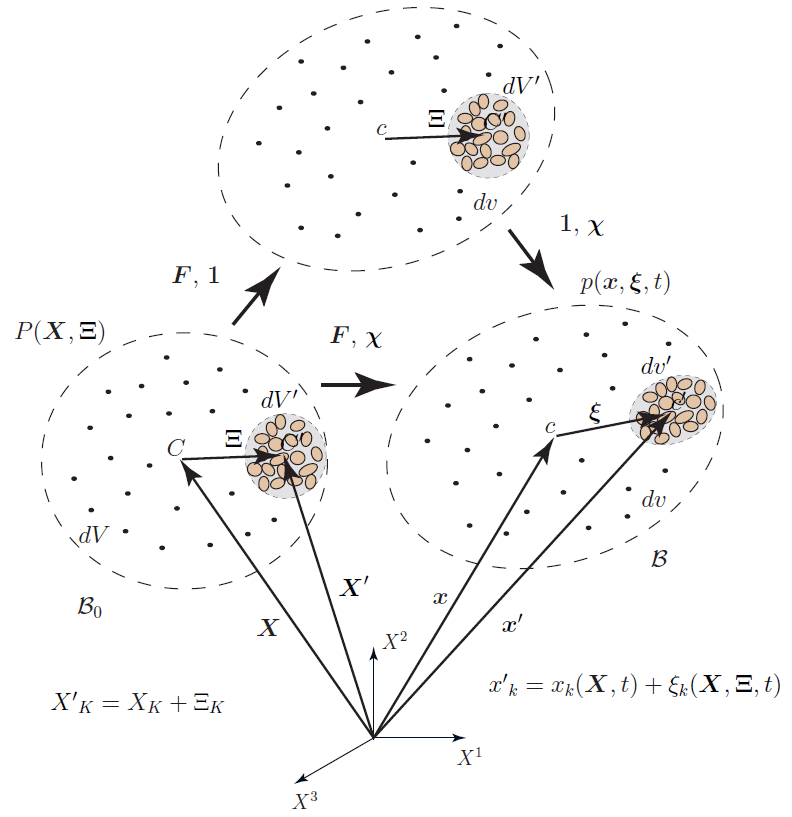
\includegraphics[width=0.9\textwidth]{micromorphic.png}
\end{figure}
\end{column}
\end{columns}
\end{frame}

\begin{frame}{Deformation Gradient Derivation}
\begin{align*}
\VEC{X}' &= \VEC{X}+\VEC{\Xi}\\
\VEC{x}' &= \VEC{x}+\VEC{\xi}\\
\end{align*}

We assume that $\LTN{\Xi_{I}} << 1$ and that a linear mapping $\TEN{\Xi}$ exists such that

\begin{align*}
\xi_i &= \chi_{iI} \Xi_I
\end{align*}

The deformation gradient $\TEN{F}$ is defined such that
\begin{align*}
F_{iI} &= \frac{\partial x_i}{\partial X_I}\\
\end{align*}
\end{frame}

\begin{frame}{Deformation Gradient Derivation}

We are searching for the mapping of $\VEC{X}'$ to $\VEC{x}'$ which we define as $\TEN{F}'$. We compute this via
\begin{align*}
F_{iI}' &= \frac{\partial}{\partial X_I'} \left\{x_i + \xi_i\right\}\\
&= \frac{\partial x_i}{\partial X_L}\frac{\partial X_L}{\partial X_I'} + \frac{\partial}{\partial X_I'} \left\{\chi_{iK}\Xi_{K}\right\}\\
&= F_{iL} \frac{\partial X_L}{\partial X_I'} + \frac{\partial \chi_{iK}}{\partial X_L}\frac{\partial X_L}{\partial X_I'}\Xi_{K} + \chi_{iK} \frac{\partial \Xi_K}{\partial X_L}\frac{\partial X_L}{\partial X_I'}\\
&= \left(F_{iL} + \frac{\partial \chi_{iK}}{\partial X_L}\Xi_{K} + \chi_{iK} \frac{\partial \Xi_K}{\partial X_L}\right)\frac{\partial X_L}{\partial X_I'}\\
&= \left(F_{iL} + \frac{\partial \chi_{iK}}{\partial X_L}\Xi_{K} + \chi_{iK} \frac{\partial \Xi_K}{\partial X_L}\right)\left(\delta_{LI} - \frac{\partial \Xi_L}{\partial X_I'}\right)\\
\end{align*}

\end{frame}

\begin{frame}{Deformation Gradient Derivation}
\begin{align*}
F_{iI}' &= F_{iI} + \frac{\partial \chi_{iK}}{\partial X_I} \Xi_K + \chi_{iK}\frac{\partial \Xi_K}{\partial X_I} - \left(F_{iL} + \frac{\partial \chi_{iK}}{\partial X_L}\Xi_{K} + \chi_{iK} \frac{\partial \Xi_K}{\partial X_L}\right)\frac{\partial \Xi_L}{\partial X_I'}\\
\end{align*}
We now do the following
\begin{align*}
\frac{\partial \Xi_I}{\partial X'_J} &= \frac{\partial \Xi_I}{\partial X_K} \frac{\partial X_K}{\partial X_J'} = \frac{\partial \Xi_I}{\partial X_K} \frac{\partial X_J'}{\partial X_K}^{-1}\\
\Rightarrow\ \frac{\partial \Xi_I}{\partial X'_J} &= \frac{\partial \Xi_I}{\partial X_K} \frac{\partial X_K}{\partial X_J'} = \frac{\partial \Xi_I}{\partial X_K} \left( \delta_{JK} + \frac{\partial \Xi_J}{\partial X_K}\right)^{-1}\\
\end{align*}
\end{frame}

\begin{frame}{Deformation Gradient Derivation}
If the gradient of the microstructural internal length $\VEC{\Xi}$ with respect to $\VEC{X}$ is small
\begin{align*}
\left( \delta_{JK} + \frac{\partial \Xi_J}{\partial X_K}\right)^{-1} &\approx \left( \delta_{KJ} - \frac{\partial \Xi_K}{\partial X_J}\right)\\
\Rightarrow\frac{\partial \Xi_I}{\partial X'_J} &\approx \frac{\partial \Xi_I}{\partial X_K} \left( \delta_{KJ} - \frac{\partial \Xi_K}{\partial X_J}\right) \approx \frac{\partial \Xi_I}{\partial X_J}\\
\end{align*}

\end{frame}

\begin{frame}{Deformation Gradient Derivation}

So what does this assumption mean?

\begin{itemize}
\item $\Xi$ is more or less the same at every location in the body $\mathcal{B}$.
\item Thus, the variation in the mass \textit{distribution} is small in each $dV$ (not necessarily the variation of the mass itself)
\item One could argue however that in an integral the $dV'$ region is, ``roving,'' and so any large, non-local change in density would be problematic
\item An example is if the substructure is \textit{periodic}
\end{itemize}

If this is true
\begin{align*}
F_{iI}' &= F_{iI} + \frac{\partial \chi_{iK}}{\partial X_I} \Xi_K - \left(F_{iL} + \frac{\partial \chi_{iK}}{\partial X_L}\Xi_{K} - \chi_{iL}\right)\frac{\partial \Xi_L}{\partial X_I}\\
\end{align*}

\end{frame}

\begin{frame}{Deformation Gradient Derivation}
If this isn't true then we can write
\begin{align*}
\frac{\partial \Xi_L}{\partial X_I'} &= \frac{\partial \Xi_L}{\partial X_M} \left( \delta_{IM} + \frac{\partial \Xi_I}{\partial X_M}\right)^{-1}\\
F_{iI}' &= F_{iI} + \frac{\partial \chi_{iK}}{\partial X_I} \Xi_K + \chi_{iL}\frac{\partial \Xi_L}{\partial X_I}\\
&\ - \left(F_{iL} + \frac{\partial \chi_{iK}}{\partial X_L}\Xi_{K} + \chi_{iK} \frac{\partial \Xi_K}{\partial X_L}\right)\frac{\partial \Xi_L}{\partial X_M} \left( \delta_{IM} + \frac{\partial \Xi_I}{\partial X_M}\right)^{-1}\\
\end{align*}
which is significantly more complicated than the periodic case though it still does not involve any derivatives with respect to $\VEC{X}'$.
\end{frame}

\begin{frame}{Deformation Gradient Derivation}
%Qualitatively I am not sure exactly what $\frac{\partial \VEC{\Xi}}{\partial \VEC{X}}$ actually is.
$\VEC{\Xi}$ points to the center of mass of the differential volume. Some cases where the gradient would be significant are
\begin{itemize}
\item A differential volume which is located in the transition between two or more materials with dissimilar densities such as the transition between a fiber and the matrix in a composite. Or between a void and some material. This region will be highly localized
\item A single material with a significant localized variation in density.
\end{itemize}
In most cases, the assumption that $\LTN{\frac{\partial \VEC{\Xi}}{\partial \VEC{X}}}<<1$ is likely a correct one especially as $dV',\VEC{\Xi} \to 0,\VEC{0}$. In any case, this is easy to check when analyzing some Direct Numerical Simulation (DNS).
\end{frame}

%\begin{frame}{1D $\VEC{\Xi}$ values}
%
%For a one dimensional bar of constant area and two regions of density separated by the Heaviside function we can compute $\VEC{\Xi}$ (here a scalar) via
%\begin{align*}
%\Xi &= x'-x = x' - \frac{\int_{x_{lb}}^{0} \rho_1 \hat{x} d\hat{x} + \int_0^{x_{ub}} \rho_2 \hat{x} d\hat{x}}{\int_{x_{lb}}^{0} \rho_1 d\hat{x} + \int_{0}^{x_{ub}} \rho_2 d\hat{x}}\\
%&= x' - \frac{1}{2}\frac{\rho_2 x_{ub}^2 - \rho_1 x_{lb}^2 }{\rho_2 x_{ub} - \rho_1x_{lb}}
%\end{align*}
%
%where, in this case, $\rho$ is the density per unit length and $\Xi$, $x'$, and $x$ are scalars because it is in 1D.
%
%\end{frame}
%
%\begin{frame}{1D $\VEC{\Xi}$ values}
%
%If we are sampling at some constant $dV' = x_{ub} - x_{lb}$
%
%\end{frame}

\begin{frame}{Balance of Mass for (Single Phase) Micromorphic Theory}

The mass of the micro-element can be defined as
\begin{align*}
m' &= \int_{dv} \rho' dv' = \int_{dV} \rho_0' dV'\\
\end{align*}

So the conservation of mass for a non-reacting material with no additional mass source becomes

\begin{align*}
\frac{Dm'}{Dt} &= 0\\
&= \frac{D}{Dt} \int_{dv} \rho' dv' = \int_{dV} \frac{D}{Dt} J' \rho' dV = 0\\
\end{align*}

\end{frame}

\begin{frame}{Balance of Mass for (Single Phase) Micromorphic Theory}

We now can make a choice for the representation of this term. Either
\begin{align*}
0 &= \int_{dV} \frac{D}{Dt} \rho_0' dV \Rightarrow\ \frac{D \rho_0'}{Dt} = 0\\
\end{align*}

or
\begin{align*}
0 &= \int_{dV} \frac{D}{Dt} \left(\rho' J'\right) dV\\
&= \int_{dV} \left(\frac{D \rho'}{D t} J' + \rho' \frac{D J'}{D t}\right) dV\\
\end{align*}

\end{frame}

\begin{frame}{Balance of Mass for (Single Phase) Micromorphic Theory}

Who is $\frac{DJ'}{Dt}$? From the definition of the derivative of a scalar valued tensor function
\begin{align*}
\frac{D J'}{Dt} &= \frac{\partial J}{\partial F_{iI}'} \frac{D F_{iI}'}{Dt}\\
\frac{\partial J}{\partial F_{iI}'} &= J' \left(F_{iI}'\right)^{-T} = J' \frac{\partial X_I'}{\partial x_i'}\\
\Rightarrow\ \frac{DJ'}{Dt} &= J' \frac{\partial X_I'}{\partial x_i'} \frac{\partial \dot{x}_i'}{\partial X_I} = J' \frac{\partial \dot{x}_i'}{\partial x_i'} = J' \frac{\partial v_i'}{\partial x_i'}
\end{align*}

where $\VEC{v}'$ is the micro-velocity in the current configuration.

\end{frame}

\begin{frame}{Balance of Mass for (Single Phase) Micromorphic Theory}

Note that we can prove
\begin{align*}
\frac{\partial J}{\partial F_{iI}'} &= J' \left(F_{iI}\right)^{-T}\\
\end{align*}

via the definition that
\begin{align*}
\frac{\partial \phi}{\partial A_{ij}}B_{ij} &= \lim_{s \to 0} \left\{\frac{\partial}{\partial s} \phi\left(A_{ij} + s B_{ij}\right) \right\}
\end{align*}

where $B_{ij}$ is arbitrary.

\end{frame}

\begin{frame}{Balance of Mass for (Single Phase) Micromorphic Theory}
Therefore
\begin{align*}
\frac{\partial J}{\partial F_{iI}'}B_{iI} &= \lim_{s \to 0} \left\{\frac{\partial}{\partial s}\det\left(F_{iI}' + s B_{iI}\right)\right\}\\
&= \lim_{s \to 0} \left\{\frac{\partial}{\partial s}\det\left(s F_{iM}' \left(\frac{1}{s}\delta_{Mj} +  \left(F_{kM}'\right)^{-1} B_{kI}\right)\right)\right\}\\
&= \lim_{s \to 0} \left\{\frac{\partial}{\partial s}\left[\det \left(s F_{iM}'\right) \det \left(\frac{1}{s}\delta_{Mj} +  \left(F_{kM}'\right)^{-1} B_{kI}\right)\right]\right\}\\
&= \lim_{s \to 0} \left\{\frac{\partial}{\partial s}\left[s^3 J' \det \left(\frac{1}{s}\delta_{Mj} +  \left(F_{kM}'\right)^{-1} B_{kI}\right)\right]\right\}\\
\end{align*}

\end{frame}

\begin{frame}{Balance of Mass for (Single Phase) Micromorphic Theory}

Noting that we can write
\begin{align*}
\det \left( \lambda \delta_{ij} + A_{ij}\right) &= \lambda^3 + \lambda^2 I_1\left(A_{ij}\right) + \lambda I_2\left(A_{ij}\right) + I_3\left(A_{ij}\right)\\
\end{align*}

we expand
\begin{align*}
\det\left(\frac{1}{s} \delta_{Mj} + \left(F_{kM}'\right)^{-1} B_{kl} \right) &= \frac{1}{s^3} + \frac{1}{s^2} I_1 + \frac{1}{s} I_2 + I_3\\
\end{align*}

Where
\begin{align*}
I_1 &= \left(F_{kM}'\right)^{-1} B_{kM}\\
\end{align*}

\end{frame}

\begin{frame}{Balance of Mass for (Single Phase) Micromorphic Theory}

Now we write
\begin{align*}
\frac{\partial J'}{\partial F_{iI}'}B_{iI} &= \lim_{s \to 0} \left\{\frac{\partial}{\partial s}\left[ J' \left(1 + sI_1 + s^2 I_2 + s^3 I_3\right)\right]\right\}\\
&= \lim_{s \to 0} \left\{J' I_1 + 2 s J' I_2 + 3 s^2 I_3\right\}\\
&= J' I_1 = J' \left(F'_{kM}\right)B_{kM}\\
&= J' \left(F'_{iI} \right)^{-1} B_{iI}\\
&= J' \left(F_{iI}'\right)^{-1} B_{iI}\\
\Rightarrow\ \frac{\partial J'}{\partial F_{iI}'} &= J' \left(F_{iI}'\right)^{-T}\\
\end{align*}

where the transpose arises because $A_{ij} B_{ij} = \TEN{A}:\TEN{B} = \text{tr}\left(\TEN{A}^{T} \cdot \TEN{B}\right)$.

\end{frame}

\begin{frame}{Balance of Mass for (Single Phase) Micromorphic Theory}

The balance of mass therefore becomes
\begin{align*}
0 &= \int_{dV} \left(\frac{D \rho'}{Dt} J' + \rho' J' \frac{\partial v_i'}{\partial x_i'}\right) dV'\\
&= \int_{dv} \left(\frac{D \rho'}{Dt} + \rho' \frac{\partial v_i'}{\partial x_i'}\right) dv'\\
\end{align*}

If we insist that this is observed pointwise
\begin{align*}
\frac{D \rho'}{Dt} + \rho' \frac{\partial v_i'}{\partial x_i'} &= 0\\
\end{align*}

\end{frame}

\begin{frame}{Balance of Mass for (Single Phase) Micromorphic Theory}

We now define the average density over the micro-volume as
\begin{align*}
\rho dv &\defeq \int_{dv} \rho' dv'\\
\end{align*}

The total mass of the body is therefore

\begin{align*}
m &= \int_{\mathcal{B}} \rho dv = \int_{\mathcal{B}} \left[\int_{dv} \rho' dv'\right] = \int_{\mathcal{B}_0} \left[\int_{dV} \rho' J' dV'\right]\\
\Rightarrow\ \frac{Dm}{Dt} &= \int_{\mathcal{B}_0} \left[\int_{dV} \frac{D}{Dt} \left(\rho' J' \right) dV' \right] = \int_{\mathcal{B}_0} \left[\int_{dV} \left(\frac{D\rho'}{Dt}J' + \rho'\frac{D J'}{Dt} \right) dV' \right]\\
\end{align*}

We know from before that $\frac{D\rho'}{Dt}J' + \rho'\frac{D J'}{Dt}  = 0$.

\end{frame}

\begin{frame}{Balance of Mass for (Single Phase) Micromorphic Theory}

We can also write
\begin{align*}
\frac{Dm}{Dt} = 0 &= \frac{D}{Dt} \int_{\mathcal{B}} \rho dv = \frac{D}{Dt} \int_{\mathcal{B}_0} \rho J dV\\
&= \int_{\mathcal{B}_0} \left[\frac{D\rho}{Dt} J + \rho \frac{DJ}{Dt}\right] dV\\
&= \int_{\mathcal{B}} \left[\frac{D\rho}{Dt} + \frac{\partial v_i}{\partial x_i}\right] dv\\
\end{align*}

And we can localize this to find
\begin{align*}
\frac{D\rho}{Dt} + \frac{\partial v_i}{\partial x_i} &= 0\\
\end{align*}
\end{frame}

\begin{frame}{Inertia of the Micro-Element}

Because we defined $\VEC{\Xi}$ as the location of the mass center of $dV'$ relative to the mass center of $dV$ we can write
\begin{align*}
\int_{dV} \rho' \Xi_I dV' &= 0\\
\end{align*}

We can define the micro-moment of inertia in the reference configuration of $dV$ via
\begin{align*}
\rho_0 I_{IJ} dV &\defeq \int_{dV} \rho_0' \Xi_{I} \Xi_{J} dV'
\end{align*}
 
\end{frame}

\begin{frame}{Inertia of the Micro-Element}

In the current configuration
\begin{align*}
\rho i_{ij} dv &\defeq \int_{dv} \rho' \xi_i \xi_j dv' = \int_{dv} \rho' \chi_{iI} \Xi_I \chi_{jJ} \Xi_J dv'\\
\end{align*}

because the deformation of $dv$ is affine $\TEN{\chi} \neq \TEN{\chi}(\VEC{x})$ so
\begin{align*}
\rho i_{ij} dv &\defeq \int_{dv} \rho' \xi_i \xi_j dv' = \chi_{iI} \chi_{jJ} \int_{dV} \rho_0' \Xi_I \Xi_J dV' = \chi_{iI} \chi_{jJ} \rho_0 I_{IJ} dV\\
\Rightarrow\ i_{ij} &= \chi_{iI} \chi_{jJ} I_{IJ} \frac{\rho_0}{\rho} \frac{dV}{dv} = \chi_{iI} \chi_{jJ} I_{IJ} \frac{J \rho}{\rho} \frac{dV}{J dV}\\
i_{ij} &= \chi_{iI} \chi_{jJ} I_{IJ}\\
\Rightarrow\ \TEN{i} &= \TEN{\chi} \cdot \TEN{I} \cdot \TEN{\chi}^T\\
\end{align*}

\end{frame}


\begin{frame}{Balance of Micro-Inertia}
We can now write the balance the inertia on the micro-scale via
\begin{align*}
\frac{D}{Dt} \int_{\mathcal{B}_0} \rho_0 I_{IJ} dV &= \int_{\mathcal{B}_0} \rho_0 \frac{D I_{IJ}}{Dt} dV = 0\\
\end{align*}



We can write
\begin{align*}
\frac{D}{Dt}\left[\chi_{iI} \chi_{jJ}I_{IJ}\right] &= \frac{D i_{ij}}{Dt}\\
\dot{\chi}_{iI} \chi_{jJ} I_{IJ} + \chi_{iI} \dot{\chi}_{jJ} I_{IJ} + \chi_{iI} \chi_{jJ} \frac{DI_{IJ}}{Dt} &= \frac{D i_{ij}}{Dt}\\
\chi_{iI} \chi_{jJ} \frac{D I_{IJ}}{Dt} &= \frac{D i_{ij}}{Dt} - \dot{\chi}_{iI} \chi_{jJ} I_{IJ} - \chi_{iI} \dot{\chi}_{jJ} I_{IJ}\\
\frac{D I_{IJ}}{Dt} &= \chi_{Li}^{-1} \chi_{Jj}^{-1} \left[\frac{D i_{ij}}{Dt} - \dot{\chi}_{iI} \chi_{jJ} I_{IJ} - \chi_{iI} \dot{\chi}_{jJ} I_{IJ}\right]\\
\end{align*}

\end{frame}

\begin{frame}{Balance of Micro-Inertia}

Furthermore
\begin{align*}
\frac{D I_{IJ}}{Dt} &= \chi_{Li}^{-1} \chi_{Jj}^{-1} \left[\frac{D i_{ij}}{Dt} - \dot{\chi}_{iI} \chi_{jJ} \chi_{Ik}^{-1} \chi_{Jm}^{-1} i_{km} - \chi_{iI} \dot{\chi}_{jJ} \chi_{Ik}^{-1} \chi_{Jm}^{-1} i_{km}\right]\\
&= \chi_{Li}^{-1} \chi_{Jj}^{-1} \left[\frac{D i_{ij}}{Dt} - \dot{\chi}_{iI} \chi_{Ik}^{-1} \delta_{jm} i_{km} - \dot{\chi}_{jJ} \delta_{ik} \chi_{Jm}^{-1} i_{km}\right]\\
&= \chi_{Li}^{-1} \chi_{Jj}^{-1} \left[\frac{D i_{ij}}{Dt} - \dot{\chi}_{iI} \chi_{Ik}^{-1} i_{kj} - \dot{\chi}_{jJ} \chi_{Jm}^{-1} i_{im}\right]\\
\end{align*}

\end{frame}

\begin{frame}{Balance of Micro-Inertia}

Note that
\begin{align*}
\dot{\xi}_i &= \dot{\chi}_{iI} \Xi_I = \dot{\chi}_{iI} \chi_{Ij}^{-1} \xi_j\\
\nu_{ij} &\defeq \dot{\chi}_{iI}\chi_{Ij}^{-1}\\
\Rightarrow\ \chi_{iI} &= \nu_{ij} \chi_{jI}\\
\end{align*}



Meaning
\begin{align*}
\frac{D I_{IJ}}{Dt} &= \chi_{Li}^{-1} \chi_{Jj}^{-1} \left[\frac{D i_{ij}}{Dt} - \nu_{ik} i_{kj} - \nu_{jm} i_{im}\right]\\
\end{align*}
\end{frame}

\begin{frame}{Balance of Micro-Inertia}

Meaning
\begin{align*}
\int_{\mathcal{B}_0} \rho_0 \frac{D I_{IJ}}{Dt} dV = \int_{\mathcal{B}_0} \rho_0 \chi_{Li}^{-1} \chi_{Jj}^{-1} \left[\frac{D i_{ij}}{Dt} - \nu_{ik} i_{kj} - \nu_{jm} i_{im}\right] dV = 0\\
\end{align*}

or in the current configuration
\begin{align*}
\int_{\mathcal{B}} \rho \frac{D I_{IJ}}{Dt} dv = \int_{\mathcal{B}} \rho \chi_{Li}^{-1} \chi_{Jj}^{-1} \left[\frac{D i_{ij}}{Dt} - \nu_{ik} i_{kj} - \nu_{jm} i_{im}\right] dv = 0\\
\end{align*}

Localizing this integral and assuming that $\rho \chi_{Li}^{-1} \chi_{Jj}^{-1}$ is arbitrary
\begin{align*}
\frac{D i_{ij}}{Dt} - \nu_{ik} i_{kj} - \nu_{jm} i_{im} &= 0\\
\end{align*}

\end{frame}

\begin{frame}{Balance of Linear and Angular Momentum for the Micro-Element}

The balance of linear and angular momentum for the micro-element is
\begin{align*}
\sigma_{ij,i}' + \rho'\left(f_{j}'-a_j'\right) &= 0\\
\sigma_{ij}' &= \sigma_{ji}'\\
\end{align*}

This means that at the micro-scale the Cauchy stress is symmetric.

\end{frame}

\begin{frame}{Balance equations for Micromorphic Theory}

We can define the balance equations for the macro-scale using the following approach
\begin{align*}
\int_{\mathcal{B}} \left\{\int_{dv} \phi' \left[\sigma_{ij,i}' + \rho'\left(f_j' - a_j'\right) \right]dv'\right\} &= 0\\
\int_{\mathcal{B}} \left\{\int_{dv} \left[\phi'\sigma_{ij,i}' + \phi'\rho'\left(f_j' - a_j'\right) \right]dv'\right\} &= 0\\
\end{align*}

where $\phi'$ is some weighting function which we will change to explore different momentum balance conditions.

\end{frame}

\begin{frame}{Balance equations for Micromorphic Theory}
Using the chain rule
\begin{align*}
\phi' \sigma_{ij,i}' &= \left(\phi' \sigma_{ij}'\right)_{,i} - \phi_{,i}' \sigma_{ij}'\\
\end{align*}

Meaning
\begin{align*}
\int_{\mathcal{B}} \left\{\int_{dv} \left[ \left(\phi' \sigma_{ij}'\right)_{,i} - \phi_{,i}' \sigma_{ij}' + \phi'\rho'\left(f_j' - a_j'\right) \right]dv'\right\} &= 0\\
\int_{\mathcal{B}} \left\{\int_{da} \phi' \sigma_{ij}' n_i' da'\right\}dv + \int_{\mathcal{B}} \left\{\int_{dv} \left[ - \phi_{,i}' \sigma_{ij}' + \phi'\rho'\left(f_j' - a_j'\right) \right]dv'\right\} &= 0\\
\end{align*}
\end{frame}

\begin{frame}{Balance equations for Micromorphic Theory}

Note that

\begin{align*}
\int_{\mathcal{B}} \left\{\int_{da} \phi' \sigma_{ij}' n_i' da' \right\} dv &= \int_{\partial \mathcal{B}} \left\{\int_{da} \phi' \sigma_{ij}' n_i' da' \right\} da
\end{align*}

if the internal tractions must be balanced between the micro-areas. If this is not satisfied the integral would need to be computed over the resulting, ``skeleton.'' It might be more appropriate to not make this simplification until $\phi'$ has been given form.

\end{frame}

\begin{frame}{Balance of Linear Momentum}

We obtain the macro-balance of linear momentum by letting $\phi'=1$
\begin{align*}
\int_{\partial \mathcal{B}} \left\{\int_{da}  \sigma_{ij}' n_i' da'\right\} + \int_{\mathcal{B}} \left\{\int_{dv} \left[\rho'\left(f_j' - a_j'\right) \right]dv'\right\} &= 0\\
\sigma_{ij}n_i da &\defeq \int_{da} \sigma_{ij}'n_i' da'\\
\rho f_j dv &\defeq \int_{dv} \rho' f_j' dv'\\
\rho a_j dv &\defeq \int_{dv} \rho' a_j' dv'\\
\end{align*}

In other words, we define the macro traction, body force, and inertial force as the averages (area and volumes respectively) of the corresponding micro values.

\end{frame}

\begin{frame}{Balance of Linear Momentum}

This means we can write
\begin{align*}
\int_{\partial \mathcal{B}} \sigma_{ij} n_i da + \int_{\mathcal{B}} \rho \left(f_j - a_j \right) dv &= 0\\
\int_{\mathcal{B}} \left[\sigma_{ij,i} + \rho\left(f_j - a_j \right) \right]dv &= 0\\
\end{align*}

Asserting this is true pointwise
\begin{align*}
\sigma_{ij,i} + \rho\left(f_j - a_j \right) &= 0\\
\end{align*}

\end{frame}

\begin{frame}{Balance of Angular Momentum}

Letting $\phi' = \epsilon_{mkj} x_k'$ and recalling that $x_k' = x_k + \xi_k$ we can solve for the balance of angular momentum
\begin{align*}
&\int_{\partial \mathcal{B}} \left\{\int_{da} \epsilon_{mkj} x_k' \sigma_{ij}' n_i' da'\right\} +\\
&\int_{\mathcal{B}} \left\{\int_{dv} \left[ - \epsilon_{mkj} \delta_{ki} \sigma_{ij}' + \epsilon_{mkj} x_k'\rho'\left(f_j' - a_j'\right) \right]dv'\right\} = 0\\
&\int_{\partial \mathcal{B}} \left\{\int_{da} \epsilon_{mkj} x_k' \sigma_{ij}' n_i' da'\right\} +\\
&\int_{\mathcal{B}} \left\{\int_{dv} \left[ - \epsilon_{mkj} \sigma_{kj}' + \epsilon_{mkj} x_k'\rho'\left(f_j' - a_j'\right) \right]dv'\right\} = 0\\
\end{align*}

\end{frame}

\begin{frame}{Balance of Angular Momentum}

We note that
\begin{align*}
a_j' &= \frac{D^2}{Dt^2}\left(x_j + \xi_j\right)\\
&= \ddot{x}_j + \ddot{\xi}_j\\
\ddot{\xi}_j = \frac{D}{Dt}\dot{\xi}_j &= \frac{D}{Dt}\left(\nu_{jk}\xi_k\right)\\
&= \dot{\nu}_{jk}\xi_k + \nu_{jk} \dot{\xi}_k\\
&= \dot{\nu}_{jk} \xi_k + \nu_{jk} \nu_{kn} \xi_n\\
&= \left(\dot{\nu}_{jk} + \nu_{jn}\nu_{nk}\right)\xi_k\\
\end{align*}

\end{frame}

\begin{frame}{Balance of Angular Momentum}

The first term of the balance of angular momentum becomes
\begin{align*}
\int_{\partial \mathcal{B}} \left\{\int_{da} \epsilon_{mkj} x_k' \sigma_{ij}' n_i' da'\right\} &= \int_{\partial \mathcal{B}} \left\{\int_{da} \epsilon_{mkj} \left(x_k + \xi_k\right) \sigma_{ij}'n_i' da' \right\}\\
&= \int_{\partial \mathcal{B}} \epsilon_{mkj} x_k \left\{\int_{da} \sigma_{ij}'n_i' da'\right\}\\
&\ + \int_{\partial \mathcal{B}} \epsilon_{mkj}\left\{\int_{da} \xi_k \sigma_{ij}'n_i' da' \right\}\\
\end{align*}

\end{frame}

\begin{frame}{Balance of Angular Momentum}

Now we make the definition
\begin{align*}
m_{ijk}n_i da &\defeq \int_{da} \sigma_{ij}' \xi_k n_i da'\\
\end{align*}

where $m_{ijk}$ is a higher order couple stress. This allows us to write
\begin{align*}
\int_{\partial \mathcal{B}} \left\{\int_{da} \epsilon_{mkj} x_k' \sigma_{ij}' n_i' da'\right\} &= \epsilon_{mkj} \int_{\partial \mathcal{B}} \left[x_k \sigma_{ij} n_i da +  m_{ijk} n_i \right]da\\
&= \epsilon_{mkj}\int_{\mathcal{B}} \left[\delta_{ki}\sigma_{ij} - x_k \sigma_{ij,i} + m_{ijk,i}\right] dv\\
&= \epsilon_{mkj}\int_{\mathcal{B}} \left[\sigma_{kj} - x_k \sigma_{ij,i} + m_{ijk,i}\right] dv\\
\end{align*}

\end{frame}

\begin{frame}{Balance of Angular Momentum}

Making the definition
\begin{align*}
s_{ij} dv &\defeq \int_{dv} \sigma_{ij}' dv'\\
\end{align*}

the second term of the balance of angular momentum
\begin{align*}
\int_{\mathcal{B}} \int_{dv}  \epsilon_{mkj} \sigma_{kj}' dv' &= \int_{\mathcal{B}} \epsilon_{mkj} \int_{dv} \sigma_{kj}' dv'\\
&= \int_{\mathcal{B}} \epsilon_{mkj} s_{kj} dv\\
\end{align*}

where $s_{ij}$ is the symmetric micro-stress tensor.
\end{frame}

\begin{frame}{Balance of Angular Momentum}

We can now write
\begin{align*}
\epsilon_{ijk}\int_{\mathcal{B}} \bigg\{\left(\sigma_{kj} + m_{ijk,i} - s_{kj}\right) dv + &\int_{dv}\big[\rho' \xi_k f_j'-\rho' \xi_k a_j'\\
&- x_k \left(\sigma_{ij,i} + \rho' \left(f_j' - a_j'\right)\right) \big] dv'\bigg\} = 0\\
\end{align*}

we can cancel out the balance of linear momentum to find
\begin{align*}
\epsilon_{ijk}\int_{\mathcal{B}} \bigg\{\left(\sigma_{kj} + m_{ijk,i} - s_{kj}\right)dv + \int_{dv}\big[&\rho' \xi_k f_j'-\rho' \xi_k a_j' \big]dv'\bigg\} = 0\\
\end{align*}

\end{frame}

\begin{frame}{Balance of Angular Momentum}

We define
\begin{align*}
\rho l_{jk} dv &= \int_{dv} \rho' \xi_k f_j' dv'\\
\end{align*}

as the body force couple. Now we turn our attention to
\begin{align*}
\int_{dv} \rho' \xi_k a_j' dv' &= \int_{dv}\rho' \left[\xi_k \ddot{x}_j + \xi_k \ddot{\xi}_j\right] dv'\\
&= \ddot{x}_j \int_{dv} \rho' \xi_k dv' + \int_{dv} \rho' \xi_k \ddot{\xi}_j dv'\\
\end{align*}

\end{frame}

\begin{frame}{Balance of Angular Momentum}

Because $\xi_k$ is defined relative to the centroid of $dv$
\begin{align*}
\ddot{x}_j \int_{dv} \rho' \xi_k dv' &= 0\\
\end{align*}

We then define
\begin{align*}
\rho \omega_{jk} dv &\defeq \int_{dv} \rho' \xi_k \ddot{\xi}_j dv'\\
\end{align*}

where $\omega_{kj}$ is the micro-spin inertia.

\end{frame}

\begin{frame}{Balance of Angular Momentum}

The balance of angular momentum is therefore
\begin{align*}
\epsilon_{ijk}\int_{\mathcal{B}} \bigg\{\sigma_{kj} + m_{ijk,i} - s_{kj} + \rho \left(l_{jk} - \omega_{jk}\right)\bigg\} = 0\\
\end{align*}

Recognizing that $\epsilon_{ijk} A_{jk} = \text{asymm}\left(A_{jk}\right)$ we can write after localization
\begin{align*}
\sigma_{[kj]} + m_{i[jk],i} + \rho\left(l_{[jk]} - \omega_{[jk]}\right) &= 0\\
\end{align*}

where $A_{[ij]}$ indicates the skew/anti-symmetric part of $\TEN{A}$.

\end{frame}

\begin{frame}{Balance of the Moment of Momentum}

The balance of angular momentum indicates that the macro Cauchy stress is not symmetric unlike in standard continuum theory. This gives us an additional three equations. Because $\chi_{ij}$ has nine terms we need six more! So we insist that the first moment of momentum is balanced by setting $\phi' = x_{m}'$
\begin{align*}
&\int_{\partial \mathcal{B}} \left\{\int_{da} x_m' \sigma_{ij}' n_i' da'\right\} +\\
&\int_{\mathcal{B}} \left\{\int_{dv} \left[ - \delta_{mi} \sigma_{ij}' +  x_m'\rho'\left(f_j' - a_j'\right) \right]dv'\right\} = 0\\
&\int_{\partial \mathcal{B}} \left\{\int_{da} x_m' \sigma_{ij}' n_i' da'\right\} +\\
&\int_{\mathcal{B}} \left\{\int_{dv} \left[ - \sigma_{mj}' + x_m'\rho'\left(f_j' - a_j'\right) \right]dv'\right\} = 0\\
\end{align*}

\end{frame}

\begin{frame}{Balance of the Moment of Momentum}

This leads to the same result as the balance of angular momentum (i.e. the balance of angular momentum is \textit{included} in the balance of the first moment of momentum) except we have the full tensors. i.e. after localization
\begin{align*}
\sigma_{kj} + m_{ijk,i} - s_{kj} + \rho\left(l_{jk} - \omega_{jk}\right) &= 0\\
\end{align*}

or nine equations for our nine additional unknowns in $\chi_{ij}$.

\end{frame}

\begin{frame}{Balance of Energy for Micromorphic Theory}

Assuming that the classical balance of energy holds in the micro-element, we can write the energy of $dv$ as
\begin{align*}
\int_{dv} \rho' \dot{e}' dv' &= \int_{dv} \left(\sigma_{ij}' v_{i,j}' - q_{i,i}' + \rho' r' \right) dv'\\
\end{align*}

where $\dot{e}'$ is the rate of change of the micro-internal energy per unit mass, $v_{i,j}$ is the micro-velocity gradient, $q_i'$ is the micro-heat flux, and $r'$ is the micro-heat source density per unit mass. We can compute the balance of energy for the body $\mathcal{B}$ via
\begin{align*}
\int_{\mathcal{B}} \left\{\int_{dv} \rho' \dot{e}' dv'\right\} &= \int_{\mathcal{B}}\left\{\int_{dv} \left(\sigma_{ij}' v_{j,i}' - q_{i,i}' + \rho' r' \right) dv'\right\}\\
\end{align*}

\end{frame}

\begin{frame}{Balance of Energy for Micromorphic Theory}

Using $x_i' = x_i + \xi_i$, $v_i' = v_i + \dot{\xi}_i = v_i + \nu_{ik} \xi_k$

we can write the first term as
\begin{align*}
\int_{dv} \rho' \dot{e}' dv' &= \int_{dV} \rho_0' \dot{e}' dV' = \frac{D}{Dt} \int_{dV} \rho_0' e' dV'\\
\rho_0 e dV &\defeq \int_{dV} \rho_0' e' dV'\\
&= \rho e dv\\
\end{align*}

where $e$ is the macro-energy density per unit mass.

\end{frame}

\begin{frame}{Balance of Energy for Micromorphic Theory}

The second term becomes
\begin{align*}
\int_{dv} \sigma_{ij}' v_{j,i}' dv' &= \int_{dv}\left[ \left(\sigma_{ij} v_j'\right)_{,i} - \sigma_{ij,i} v_i' \right] dv'\\
&= \int_{da} \sigma_{ij}' v_j' n_i' da' - \int_{dv} \sigma_{ij,i} v_j dv'\\
&= \int_{da} \sigma_{ij}' \left(v_j + \nu_{jk}\xi_k\right) n_i' da' - \int_{dv} \sigma_{ij,i} \left(v_j + \nu_{jk}\xi_k\right) dv'\\
&= v_j \int_{da} \sigma_{ij}' n_i' da' + \nu_{jk}\int_{da} \sigma_{ij}' \xi_k n_i' da'\\
&\ \ \  - v_j\int_{dv} \sigma_{ij,i} dv' - \nu_{jk}\int_{dv} \sigma_{ij,i} \xi_k dv'\\
\end{align*}

\end{frame}

\begin{frame}{Balance of Energy for Micromorphic Theory}

Using our definitions from before and the micro-element balance of linear momentum
\begin{align*}
\int_{dv} \sigma_{ij}' v_{j,i}' dv' &= v_j \sigma_{ij} n_i da + \nu_{jk} m_{ijk} n_i da + v_j\int_{dv} \rho' f_j' dv' - v_j \int_{dv} \rho' a_j' dv'\\
&\ \ \   - \nu_{jk}\int_{dv} \rho'f_j' \xi_k dv' + \nu_{jk} \int_{dv} \rho' a_j' \xi_k dv'\\
&= v_j \sigma_{ij} n_i da + \nu_{jk} m_{ijk} n_i da+ v_j \rho f_j dv - v_j \rho a_j dv\\
&\ \ \   + \nu_{jk} \rho l_{jk} dv - \nu_{jk} \int_{dv} \rho'\left(a_j + \ddot{\xi_j}\right) \xi_k dv'\\
&= v_j \sigma_{ij} n_i da + \nu_{jk} m_{ijk} n_i da+ v_j \rho f_j dv - v_j \rho a_j dv\\
&\ \ \   + \nu_{jk} \rho l_{jk} dv - \nu_{jk}a_j \int_{dv}\rho' \xi_k dv' - \nu_{jk}\int_{dv} \rho'\ddot{\xi_j} \xi_k dv'\\
\end{align*}

\end{frame}

\begin{frame}{Balance of Energy for Micromorphic Theory}
Note that
\begin{align*}
\int_{dv}\rho'\xi_k dv' = 0\\
\end{align*}
So
\begin{align*}
\int_{dv} \sigma_{ij}' v_{j,i}' dv' &= v_j \sigma_{ij} n_i da + \nu_{jk} m_{ijk} n_i da+ v_j \rho f_j dv - v_j \rho a_j dv\\
&\ \ \   + \nu_{jk} \rho l_{jk} dv - \nu_{jk}\rho \omega_{jk} dv\\
\end{align*}

We also note
\begin{align*}
\int_{dv} q_{i,i}' dv' &= \int_{da} q_{i} n_i' da'\\
\end{align*}

\end{frame}

\begin{frame}{Balance of Energy for Micromorphic Theory}

Which allows us to define
\begin{align*}
q_i n_i da &\defeq \int_{da} q_i' n_i' dv'\\
\rho r &\defeq \int_{dv} \rho' r' dv'\\
\end{align*}

And so the balance of energy of the body becomes
\begin{align*}
\int_{\mathcal{B}} \rho \dot{e} dv &= \int_{\partial \mathcal{B}}\left\{ v_j \sigma_{ij} n_i + \nu_{jk} m_{ijk} n_i\right\}da - \int_{\partial \mathcal{B}} q_i n_i da\\
&\ \ \  + \int_{\mathcal{B}}\rho r dv + \int_{\mathcal{B}}\left\{v_j \rho \left(f_j - a_j\right) + \nu_{jk}\rho\left( l_{jk} - \omega_{jk}\right) \right\}dv\\
\end{align*}

\end{frame}

\begin{frame}{Balance of Energy for Micromorphic Theory}

\begin{align*}
\int_{\mathcal{B}} \rho \dot{e} dv &= \int_{\mathcal{B}}\left\{ \left(v_j \sigma_{ij}\right)_{,i} + \left(\nu_{jk} m_{ijk}\right)_{,i} + v_j \rho \left(f_j - a_j\right) + \nu_{jk}\rho\left( l_{jk} - \omega_{jk}\right) \right\}dv\\
&\ \ \  - \int_{\partial \mathcal{B}} q_i n_i da + \int_{\mathcal{B}}\rho r dv\\
&= \int_{\mathcal{B}}\bigg\{ v_{j,i} \sigma_{ij} + v_{j} \sigma_{ij,i} + \nu_{jk,i} m_{ijk} + \nu_{jk} m_{ijk,i}\\
&\ +v_j \rho \left(f_j - a_j\right) + \nu_{jk}\rho \left( l_{jk} - \omega_{jk}\right) \bigg\}dv\\
&\ \ \  - \int_{\partial \mathcal{B}} q_i n_i da + \int_{\mathcal{B}}\rho r dv\\
\end{align*}

\end{frame}

\begin{frame}{Balance of Energy for Micromorphic Theory}

\begin{align*}
\int_{\mathcal{B}} \rho \dot{e} dv &= \int_{\mathcal{B}}\bigg\{ v_{j,i} \sigma_{ij} + \nu_{jk,i} m_{ijk}\\
&\ +v_j \left[ \sigma_{ij,i} + \rho \left(f_j - a_j\right)\right]\\
&\ \ \ \nu_{jk} \left[m_{ijk,i} + \rho \left( l_{jk} - \omega_{jk}\right)\right] \bigg\}dv\\
&\ \ \  - \int_{\partial \mathcal{B}} q_i n_i da + \int_{\mathcal{B}}\rho r dv\\
&= \int_{\mathcal{B}}\bigg\{ v_{j,i} \sigma_{ij} + \nu_{jk,i} m_{ijk} + \nu_{jk} \left[s_{kj} - \sigma_{kj}\right] \bigg\}dv\\
&\ \ \  - \int_{\partial \mathcal{B}} q_i n_i da + \int_{\mathcal{B}}\rho r dv\\
\end{align*}

\end{frame}

\begin{frame}{Balance of Energy for Micromorphic Theory}

Localizing the integral we find
\begin{align*}
\rho \dot{e} &= v_{j,i} \sigma_{ij} + \nu_{jk,i} m_{ijk} + \nu_{jk}\left[s_{kj} - \sigma_{kj}\right] - q_{i,i} + \rho r\\
\end{align*}

So we have terms that have been previously observed ($v_{j,i} \sigma_{ij}$ and the heat terms) and then new terms associated with inhomogeneity in the stress of the micro-elements.

\end{frame}

\begin{frame}{The Second Law for Micromorphic Theory}

The second law is assumed to hold in the micro-element as it does in the typical continuum such that
\begin{align*}
\frac{D}{Dt}\int_{dv} \rho' \eta' dv' + \int_{da} \frac{1}{\theta'} q_{i}' n_i' da - \int_{dv} \frac{\rho' r'}{\theta'} dv &\geq 0\\ 
\end{align*}

where we have introduced $\eta'$ as the micro-entropy per unit mass and $\theta'$ as the micro-temperature.

\end{frame}

\begin{frame}{The Second Law for Micromorphic Theory}

Defining
\begin{align*}
\theta dv &\defeq \int_{dv} \theta' dv\\
\rho \dot{\eta} dv &\defeq \int_{dv} \rho' \frac{D \eta'}{Dt} dv'\\
\left(\frac{1}{\theta} q_i\right)_{,i} dv &\defeq \int_{dv} \left(\frac{1}{\theta'} q_i'\right)_{,i} dv\\
\frac{\rho r}{\theta} &\defeq \int_{dv} \frac{\rho' r'}{\theta'} dv\\
\end{align*}

\end{frame}

\begin{frame}{The Second Law for Micromorphic Theory}

We integrate over $\mathcal{B}$ to find
\begin{align*}
\int_{\mathcal{B}} \left\{\rho \dot{\eta} + \left(\frac{1}{\theta} q_i\right)_{,i} - \frac{\rho r}{\theta}\right\}dv &\geq 0\\
\int_{\mathcal{B}} \left\{\rho \dot{\eta} + \frac{1}{\theta} q_{i,i} - \frac{1}{\theta^2} q_i \theta_{,i} - \frac{\rho r}{\theta}\right\}dv &\geq 0\\
\end{align*}

Insisting it is satisfied pointwise leads to
\begin{align*}
\rho \theta \dot{\eta} + q_{i,i} - \frac{1}{\theta} q_i \theta_{,i} - \rho r &\geq 0\\
\end{align*}

\end{frame}

\begin{frame}{Introduction of the Helmholtz Free Energy}

We introduce the Helmholtz free energy as
\begin{align*}
\psi &= e - \theta \eta\\
\Rightarrow\ \dot{\psi} &= \dot{e} - \dot{\theta} \eta - \theta \dot{\eta}\\
\Rightarrow\ \rho \theta \dot{\eta} &= \rho \dot{e} - \rho \dot{\theta} \eta - \rho \dot{\psi}\\
\end{align*}

So we can rewrite the second law as
\begin{align*}
\rho \dot{e} - \rho \dot{\theta} \eta - \rho \dot{\psi} + q_{i,i} - \frac{1}{\theta} q_i \theta_i - \rho r \geq 0\\
\end{align*}

\end{frame}

\begin{frame}{Clausius-Duhem Inequality for Micromorphic Theory}

We can substitute the first law into the second via
\begin{align*}
v_{j,i} \sigma_{ij} + \nu_{jk,i} m_{ijk} + \nu_{jk}\left[s_{kj} - \sigma_{kj}\right] + q_{i,i} + \rho r\\ - \rho \dot{\theta} \eta - \rho \dot{\psi} - q_{i,i} + \frac{1}{\theta} q_i \theta_i - \rho r \geq 0\\
\Rightarrow\ v_{j,i} \sigma_{ij} + \nu_{jk,i} m_{ijk} + \nu_{jk}\left[s_{kj} - \sigma_{kj}\right]\\ - \rho \left(\dot{\theta} \eta + \dot{\psi}\right) - \frac{1}{\theta} q_i \theta_{,i}\geq 0\\
\end{align*}



\end{frame}

\begin{frame}{Micromorphic Deformation Measures}

Assuming a decomposition in the form of $F_{iI}' = F_{i\bar{I}}^eF_{\bar{I}I}^p$ we wish to define an elastic deformation measure which we do via the difference of the  squared magnitude of $d\VEC{x}'$ and $d\VEC{\bar{X}}'$ where $\bar{\cdot}$ indicates a quantity in the intermediate configuration
\begin{align*}
\left(ds'\right)^2 - \left(d\bar{S}'\right)^2 &= dx_i' dx_i' - d\bar{X}_i' d\bar{X}_i'
\end{align*} We can write
\begin{align*}
dx_i' &= dx_i + d\xi_i\\
d\bar{X}_{\bar{I}}' &= d\bar{X}_i + d\bar{\Xi}_i\\
\end{align*} so \begin{align*}
dx_i' dx_i' &= dx_i dx_i + 2 dx_i d\xi_i + d\xi_i d\xi_i\\
\end{align*}

\end{frame}

\begin{frame}{Micromorphic Deformation Measures}
Furthermore,
\begin{align*}
d\bar{X}_{\bar{I}}' d\bar{X}_{\bar{I}}' &= d\bar{X}_{\bar{I}} d\bar{X}_{\bar{I}} + 2d\bar{X}_{\bar{I}} d\bar{\Xi}_{\bar{I}} + d\bar{\Xi}_{\bar{I}} d\bar{\Xi}_{\bar{I}}\\
\end{align*}

Earlier, we defined
\begin{align*}
\xi_i &= \chi_{iI}\Xi_I\\
\end{align*}

which we extend to
\begin{align*}
\Rightarrow\ \xi_i &= \chi_{i\bar{I}}^e\chi_{\bar{I}I}^p \Xi_I\\
\end{align*}

\end{frame}

\begin{frame}{Micromorphic Deformation Measures}

meaning
\begin{align*}
\frac{\partial \xi_i}{\partial \bar{X}_{\bar{I}}} &= \frac{\partial \chi_{iI}}{\partial \bar{X}_{\bar{I}}} \Xi_I + \chi_{iI} \frac{\partial \Xi_I}{\partial \bar{X}_{\bar{I}}}\\
\Rightarrow\ d \xi_i &= \frac{\partial \chi_{iI}}{\partial \bar{X}_{\bar{I}}} \Xi_I d \bar{X}_{\bar{I}} + \chi_{i\bar{I}}^e \chi_{\bar{I}I}^p d\Xi_{I} \\
&= \left(\chi_{i\bar{K},\bar{I}}^e\chi_{\bar{K}I}^p + \chi_{i\bar{K}}^e\chi_{\bar{K}I,\bar{I}}^p \right)\Xi_I d\bar{X}_{\bar{I}} + \chi_{i\bar{I}}^e d\bar{\Xi}_{\bar{I}}\\
&= \chi_{i\bar{K},\bar{I}}^e\bar{\Xi}_{\bar{K}}d\bar{X}_{\bar{I}} + \chi_{i\bar{K}}^e\chi_{\bar{K}I,\bar{I}}^p \Xi_I d\bar{X}_{\bar{I}} + \chi_{i\bar{I}}^e d\bar{\Xi}_{\bar{I}}\\
\end{align*}

\end{frame}

\begin{frame}{Micromorphic Deformation Measures}

The full representation of $dx_i$ is therefore
\begin{align*}
dx_i &= F_{i\bar{I}}^e d\bar{X}_{\bar{I}} + \chi_{i\bar{K},\bar{I}}^e\bar{\Xi}_{\bar{K}}d\bar{X}_{\bar{I}} + \chi_{i\bar{K}}^e\chi_{\bar{K}I,\bar{I}}^p \Xi_I d\bar{X}_{\bar{I}} + \chi_{i\bar{I}}^e d\bar{\Xi}_{\bar{I}}
\end{align*}
and we can write $dx_i dx_i$ as
\begin{align*}
dx_i dx_i &= \left(F_{i\bar{I}}^e d\bar{X}_{\bar{I}} + \chi_{i\bar{K},\bar{I}}^e\bar{\Xi}_{\bar{K}}d\bar{X}_{\bar{I}} + \chi_{i\bar{K}}^e\chi_{\bar{K}I,\bar{I}}^p \Xi_I d\bar{X}_{\bar{I}} + \chi_{i\bar{I}}^e d\bar{\Xi}_{\bar{I}}\right)\\
&\ \ \ \left(F_{i\bar{J}}^e d\bar{X}_{\bar{J}} + \chi_{i\bar{L},\bar{J}}^e\bar{\Xi}_{\bar{L}}d\bar{X}_{\bar{J}} + \chi_{i\bar{L}}^e\chi_{\bar{L}J,\bar{J}}^p \Xi_J d\bar{X}_{\bar{J}} + \chi_{i\bar{J}}^e d\bar{\Xi}_{\bar{J}}\right)
\end{align*}

\end{frame}

\begin{frame}{Micromorphic Deformation Measures}

The resulting term which only includes $d\bar{X}_{\bar{I}}$ and $d\bar{X}_{\bar{J}}$ is 
\begin{align*}
T_{\bar{I}\bar{J}}^{(1)} = \bigg[& F_{i\bar{I}}^eF_{i\bar{J}}^e + F_{i\bar{I}}^e \chi_{i\bar{L},\bar{J}}^e \bar{\Xi}_{\bar{L}} + F_{i\bar{I}}^e \chi_{i\bar{L}}^e\chi_{\bar{L}J,\bar{J}}^p \Xi_{J} +\\
&F_{i\bar{J}}^e \chi_{i\bar{K},\bar{I}}\bar{\Xi}_{\bar{K}} + \chi_{i\bar{K},\bar{I}}^e \bar{\Xi}_{\bar{K}}\chi_{i\bar{L},\bar{J}}^e\bar{\Xi}_{\bar{L}} +  \chi_{i\bar{K},\bar{I}}^e\bar{\Xi}_{\bar{K}} \chi_{i\bar{L}}^e \chi_{\bar{L}J, \bar{J}}^p \Xi_{J}+\\
&F_{i\bar{J}}^e\chi_{i\bar{K}}^e\chi_{\bar{K}I,\bar{I}}^p \Xi_I + \chi_{i\bar{L},\bar{J}}^e \bar{\Xi}_{\bar{L}}\chi_{i\bar{K}}^e\chi_{\bar{K}I,\bar{I}}^p \Xi_I +\\
& \chi_{i\bar{K}}^e\chi_{\bar{K}I,\bar{I}}^p \Xi_I \chi_{i\bar{L}}^e \chi_{\bar{L}J,\bar{J}}^p \Xi_J \bigg] %d\bar{X}_{\bar{I}}d\bar{X}_{\bar{J}}\\
\end{align*}

To simplify we make the following definitions
\begin{align*}
\bar{C}_{\bar{I}\bar{J}}^e = F_{i\bar{I}}^e F_{i\bar{J}}^e,\ \bar{\Gamma}_{\bar{I}\bar{L}\bar{J}}^e = F_{i\bar{I}}^e \chi_{i\bar{L},\bar{J}}^e,\ \bar{\Psi}_{\bar{I}\bar{J}}^e = F_{i\bar{I}}^e \chi_{i\bar{J}}^e\\
\end{align*}

\end{frame}

\begin{frame}{Micromorphic Deformation Measures}

Noting that
\begin{align*}
2\text{symm}\left(\bar{\Gamma}_{\bar{I}\bar{L}\bar{J}}^e\right)\Xi_{\bar{L}} &= F_{i\bar{I}}^e \chi_{i\bar{L},\bar{J}}^e \bar{\Xi}_{\bar{L}} + F_{i\bar{J}}^e \chi_{i\bar{K},\bar{I}}\bar{\Xi}_{\bar{K}}\\
2\text{symm}\left(\bar{\Psi}_{\bar{I}\bar{L}} \chi_{\bar{L}J,\bar{J}}^e\right)\Xi_J &= F_{i\bar{I}}^e \chi_{i\bar{L}}^e\chi_{\bar{L}J,\bar{J}}^p \Xi_{J} + F_{i\bar{J}}^e\chi_{i\bar{K}}^e\chi_{\bar{K}I,\bar{I}}^p \Xi_I\\
%\chi_{i\bar{K},\bar{I}} &= \bar{\Gamma}_{\bar{M}\bar{K}\bar{I}}^e\left(F_{i\bar{M}}^e\right)^{-1}\\
%\chi_{i\bar{L},\bar{J}} &= \bar{\Gamma}_{\bar{N}\bar{L}\bar{J}}^e\left(F_{i\bar{N}}^e\right)^{-1}\\
\left(\bar{C}_{\bar{M}\bar{N}}^e\right)^{-1} \bar{\Gamma}_{\bar{M}\bar{K}\bar{I}}^e  \bar{\Gamma}_{\bar{N}\bar{L}\bar{J}}^e\bar{\Xi}_{\bar{K}} \bar{\Xi}_{\bar{L}} &= \chi_{i\bar{K},\bar{I}}^e \chi_{i\bar{L},\bar{J}}^e \bar{\Xi}_{\bar{K}} \bar{\Xi}_{\bar{L}}\\
%\chi_{i\bar{K}}^e &= \left(F_{i\bar{M}}\right)^{-1} \bar{\Psi}_{\bar{M}\bar{K}}^e\\
%\chi_{i\bar{L}}^e &= \left(F_{i\bar{N}}\right)^{-1} \bar{\Psi}_{\bar{N}\bar{L}}^e\\
\left(\bar{C}_{\bar{M}\bar{N}}^e\right)^{-1} \bar{\Psi}_{\bar{M}\bar{K}}^e \bar{\Psi}_{\bar{N}\bar{L}}^e\chi_{\bar{K}I,\bar{I}}^p \chi_{\bar{L}J,\bar{J}}^p \Xi_I\Xi_J  &= \chi_{i\bar{K}}^e \chi_{i\bar{L}}^e \chi_{\bar{K}I,\bar{I}}^p \chi_{\bar{L}J,\bar{J}}^p \Xi_I\Xi_J\\
\end{align*}

\end{frame}

\begin{frame}{Micromorphic Deformation Measures}
Also,
\begin{align*}
2\text{symm}\left(\chi_{i\bar{L},\bar{I}}^e\chi_{i\bar{K}}^e \chi_{\bar{K}I, \bar{J}}^p\right) \bar{\Xi}_{\bar{L}} \Xi_I &=\left(\chi_{i\bar{L},\bar{I}}^e\chi_{i\bar{K}}^e \chi_{\bar{K}I, \bar{J}}^p+\chi_{i\bar{L},\bar{J}}^e \chi_{i\bar{K}}^e\chi_{\bar{K}I,\bar{I}}^p \right)\bar{\Xi}_{\bar{L}} \Xi_{I}\\
&= 2\text{symm}\bigg(\left(\bar{C}_{\bar{M}\bar{N}}^e\right)^{-1}\\
&\ \ \ \ \ \ \ \bar{\Gamma}_{\bar{M}\bar{L}\bar{I}}^e \bar{\Psi}_{\bar{N}\bar{K}}^e\chi_{\bar{K}I,\bar{J}}^p\bigg)\bar{\Xi}_{\bar{L}}\Xi_I\\
\end{align*}

\end{frame}

\begin{frame}{Micromorphic Deformation Measures}

We can write
\begin{align*}
T_{\bar{I}\bar{J}}^{(1)} = \bigg[& \bar{C}_{\bar{I}\bar{J}}^e + 2\text{symm}\left(\bar{\Gamma}_{\bar{I}\bar{L}\bar{J}}^e\right)\Xi_{\bar{L}} + 2\text{symm}\left(\bar{\Psi}_{\bar{I}\bar{L}} \chi_{\bar{L}J,\bar{J}}^e\right)\Xi_J +\\
&\left(\bar{C}_{\bar{M}\bar{N}}^e\right)^{-1} \bar{\Gamma}_{\bar{M}\bar{K}\bar{I}}^e  \bar{\Gamma}_{\bar{N}\bar{L}\bar{J}}^e\bar{\Xi}_{\bar{K}} \bar{\Xi}_{\bar{L}} +\\
&2\text{symm}\bigg(\left(\bar{C}_{\bar{M}\bar{N}}^e\right)^{-1}\bar{\Gamma}_{\bar{M}\bar{L}\bar{I}}^e \bar{\Psi}_{\bar{N}\bar{K}}^e\chi_{\bar{K}I,\bar{J}}^p\bigg)\bar{\Xi}_{\bar{L}}\Xi_I +\\
& \left(\bar{C}_{\bar{M}\bar{N}}^e\right)^{-1} \bar{\Psi}_{\bar{M}\bar{K}}^e \bar{\Psi}_{\bar{N}\bar{L}}^e\chi_{\bar{K}I,\bar{I}}^p \chi_{\bar{L}J,\bar{J}}^p \Xi_I\Xi_J\bigg]% d\bar{X}_{\bar{I}}d\bar{X}_{\bar{J}}\\
\end{align*}

\end{frame}

\begin{frame}{Micromorphic Deformation Measures}

The term of $dx_i dx_i$ involving only $d\bar{\Xi}_{\bar{I}}$ and $d\bar{\Xi}_{\bar{J}}$ becomes
\begin{align*}
T_{\bar{I}\bar{J}}^{(2)} &= \chi_{i\bar{I}}^e \chi_{i\bar{J}}^e d\bar{\Xi}_{\bar{I}}d\bar{\Xi}_{\bar{J}}\\
&= \left(C_{\bar{M}\bar{N}}^e\right)^{-1} \bar{\Psi}_{\bar{M}\bar{I}}^e \bar{\Psi}_{\bar{N}\bar{J}}^e d\bar{\Xi}_{\bar{I}}d\bar{\Xi}_{\bar{J}}\\
\end{align*}

\end{frame}

\begin{frame}{Micromorphic Deformation Measures}

The term of $dx_i dx_i$ involving mixed terms of $d\bar{\VEC{\Xi}}$ and $d\bar{\VEC{X}}$ is
\begin{align*}
T_{\bar{I}\bar{J}}^{(3)} &= F_{i\bar{I}}^e \chi_{i\bar{J}}^e + \chi_{i\bar{K},\bar{I}}^e \bar{\Xi}_{\bar{K}} \chi_{i\bar{J}}^e + \chi_{i\bar{K}}^e \chi_{\bar{K}I,\bar{I}}^p \Xi_{I} \chi_{i\bar{J}}^e\\
&+\ F_{i\bar{J}}^e \chi_{i\bar{I}}^e + \chi_{i\bar{L},\bar{J}}^e \bar{\Xi}_{\bar{L}} \chi_{i\bar{I}}^e + \chi_{i\bar{L}}^e \chi_{\bar{L}J,\bar{J}}^p \Xi_{J} \chi_{i\bar{I}}^e\\
&= F_{i\bar{I}}^e \bar{\Psi}_{\bar{K}\bar{J}}^e \left(F_{i\bar{K}}^e\right)^{-1} + \left(F_{i\bar{M}}^e\right)^{-1} \bar{\Gamma}_{\bar{M}\bar{K}\bar{I}} \bar{\Xi}_{\bar{K}} \bar{\Psi}_{\bar{N}\bar{J}}^e \left(F_{i\bar{N}}^e\right)^{-1}\\
& + \left(F_{i\bar{M}}^e\right)^{-1} \bar{\Psi}_{\bar{M}\bar{K}}^e \chi_{\bar{K}I,\bar{I}}^p \Xi_{I} \bar{\Psi}_{\bar{N}\bar{J}}^e \left(F_{i\bar{N}}^e\right)^{-1}\\
&+\ F_{i\bar{J}}^e\bar{\Psi}_{\bar{K}\bar{I}}^e \left(F_{i\bar{K}}^e\right)^{-1} + \left(F_{i\bar{M}}^e\right)^{-1} \bar{\Gamma}_{\bar{M}\bar{L}\bar{J}} \bar{\Xi}_{\bar{L}} \bar{\Psi}_{\bar{N}\bar{I}}^e \left(F_{i\bar{N}}^e\right)^{-1}\\
& + \left(F_{i\bar{M}}^e\right)^{-1} \bar{\Psi}_{\bar{M}\bar{L}}^e \chi_{\bar{L}J,\bar{J}}^p \Xi_{J} \bar{\Psi}_{\bar{N}\bar{I}}^e \left(F_{i\bar{N}}^e\right)^{-1}\\
%&= 2\bigg[\bar{\Psi}_{\bar{I}\bar{J}} + \bigg]\\
\end{align*}

\end{frame}

\begin{frame}{Micromorphic Deformation Measures}
\begin{align*}
T_{\bar{I}\bar{J}}^{(3)}&= \bar{\Psi}_{\bar{I}\bar{J}}^e  + \left(\bar{C}_{\bar{M}\bar{N}}^e\right)^{-1} \bar{\Gamma}_{\bar{M}\bar{K}\bar{I}} \bar{\Xi}_{\bar{K}} \bar{\Psi}_{\bar{N}\bar{J}}^e\\
& + \left(\bar{C}_{\bar{M}\bar{N}}^e\right)^{-1} \bar{\Psi}_{\bar{M}\bar{K}}^e \chi_{\bar{K}I,\bar{I}}^p \Xi_{I} \bar{\Psi}_{\bar{N}\bar{J}}^e\\
&+\ \bar{\Psi}_{\bar{J}\bar{I}}^e + \left(\bar{C}_{\bar{M}\bar{N}}^e\right)^{-1} \bar{\Gamma}_{\bar{M}\bar{L}\bar{J}} \bar{\Xi}_{\bar{L}} \bar{\Psi}_{\bar{N}\bar{I}}^e\\
& + \left(\bar{C}_{\bar{M}\bar{N}}^e\right)^{-1} \bar{\Psi}_{\bar{M}\bar{L}}^e \chi_{\bar{L}J,\bar{J}}^p \Xi_{J} \bar{\Psi}_{\bar{N}\bar{I}}^e\\
&= 2\bigg[\bar{\Psi}_{\bar{I}\bar{J}} + \left(\bar{C}_{\bar{M}\bar{N}}^e\right)^{-1} \bar{\Gamma}_{\bar{M}\bar{K}\bar{I}} \bar{\Xi}_{\bar{K}} \bar{\Psi}_{\bar{N}\bar{J}}^e + \left(\bar{C}_{\bar{M}\bar{N}}^e\right)^{-1} \bar{\Psi}_{\bar{M}\bar{K}}^e \chi_{\bar{K}I,\bar{I}}^p \Xi_{I} \bar{\Psi}_{\bar{N}\bar{J}}^e\bigg]\\
\end{align*}
\end{frame}

\begin{frame}{Micromorphic Deformation Measures}

So the full strain measures in the intermediate configuration are
\begin{align*}
\left(dx_i'\right)^2 - \left(dS_I'\right)^2 &= d\bar{X}_{I} \left(T_{\bar{I}\bar{J}}^{(1)} - \delta_{\bar{I}\bar{J}}\right) d\bar{X}_{J}\\
&\ + d\bar{\Xi}_{I} \left(T_{\bar{I}\bar{J}}^{(2)} - \delta_{\bar{I}\bar{J}}\right) d\bar{\Xi}_{J}\\
&\ + 2d\bar{X}_{I}\left(T_{\bar{I}\bar{J}}^{(3)} - \delta_{\bar{I}\bar{J}}\right) d\bar{\Xi}_{J}\\
\end{align*}

We will use the deformation measures $\bar{C}_{\bar{I}\bar{J}},\ \bar{\Gamma}_{\bar{I}\bar{J}\bar{K}},\ \text{and}\ \bar{\Psi}_{\bar{I}\bar{J}}$ to construct our constitutive model.

\end{frame}

\begin{frame}{Kinematics of a Micromorphic Elasto/Plastic Material}

We can write the velocity gradient $\left(\frac{\partial \dot{x}_i}{\partial x_j}\right)$ in the current configuration via
\begin{align*}
l_{ij} = v_{i,j} &= \frac{\partial \dot{x}_i}{\partial x_j} =  \frac{\partial \dot{x}_i}{\partial X_J} \frac{\partial X_J}{\partial x_j}\\
\Rightarrow\ \TEN{l} &= \dot{\TEN{F}} \TEN{F}^{-1}\\
\end{align*}

For our case
\begin{align*}
l_{ij} &= \frac{D}{Dt}\left(F_{i\bar{J}}^e F_{\bar{J}J}^p\right)\left(F_{j\bar{K}}^e F_{\bar{K} J}^p\right)^{-1}\\
&= \left(\dot{F}_{i\bar{J}}^e F_{\bar{J}J}^p + F_{i\bar{J}}^e \dot{F}_{\bar{J}J}^p\right)\left(F_{ \bar{K}J}^p\right)^{-1}\left(F_{j\bar{K}}^e\right)^{-1}\\
&= \dot{F}_{i\bar{J}}^e \delta_{\bar{J}\bar{K}} \left(F_{j\bar{K}}^e\right)^{-1} + F_{i\bar{J}}^e \dot{F}_{\bar{J}J}^p\left(F_{\bar{K}J}^p\right)^{-1}\left(F_{j\bar{K}}^e\right)^{-1}\\
\end{align*}

\end{frame}

\begin{frame}{Kinematics of a Micromorphic Elasto/Plastic Material}

Defining
\begin{align*}
l_{ij}^e &\defeq \dot{F}_{i\bar{J}}^e \left(F_{j\bar{J}}^e\right)^{-1}\\
\bar{L}_{\bar{J}\bar{K}}^p &\defeq \dot{F}_{\bar{J}J}^p\left(F_{\bar{K}J}^p\right)^{-1}\\
\end{align*}
we find
\begin{align*}
l_{ij} &= l_{ij}^e + F_{i\bar{J}}^e \bar{L}_{\bar{J}\bar{K}}^p \left(F_{j\bar{K}}^e\right)^{-1}\\
&= l_{ij}^e + \frac{\partial x_i}{\partial \bar{X}_{\bar{J}}} \frac{\partial \dot{\bar{X}}_{\bar{J}}}{\partial \bar{X}_{\bar{K}}} \frac{\partial \bar{X}_{\bar{K}}}{\partial x_j}\\
&= l_{ij}^e + l_{ij}^p
\end{align*}

\end{frame}

\begin{frame}{Kinematics of a Micromorphic Elasto/Plastic Material}

where we defined
\begin{align*}
l_{ij}^p &\defeq \frac{\partial x_i}{\partial \bar{X}_{\bar{J}}} \frac{\partial \dot{\bar{X}}_{\bar{J}}}{\partial \bar{X}_{\bar{K}}} \frac{\partial \bar{X}_{\bar{K}}}{\partial x_j}
\end{align*}

as the plastic velocity gradient in the current configuration.

Similarly
\begin{align*}
\nu_{ij} &= \dot{\chi}_{iJ} \chi_{J j}^{-1}\\
&= \frac{D}{Dt}\left(\chi_{i\bar{I}}^e \chi_{\bar{I} I}^p\right)\left(\chi_{j \bar{J}}^e \chi_{\bar{J} I}^p\right)^{-1}\\
&= \left(\dot{\chi}_{i\bar{I}}^e \chi_{\bar{I}I}^p + \chi_{i\bar{I}}^e \dot{\chi}_{\bar{I}I}^p\right)\left(\chi_{\bar{J} I}^p\right)^{-1}\left(\chi_{j \bar{J}}^e\right)^{-1}
\end{align*}

\end{frame}

\begin{frame}{Kinematics of a Micromorphic Elasto/Plastic Material}

\begin{align*}
\nu_{ij} &= \dot{\chi}_{i\bar{I}}^e \delta_{\bar{I}\bar{J}}\left(\chi_{j \bar{J}}^e\right)^{-1} + \chi_{i\bar{I}}^e \dot{\chi}_{\bar{I}I}^p\left(\chi_{\bar{J} I}^p\right)^{-1}\left(\chi_{j \bar{J}}^e\right)^{-1}
\end{align*}

Defining
\begin{align*}
\nu_{ij}^e &= \dot{\chi}_{i\bar{I}}^e\left(\chi_{j \bar{I}}^e\right)^{-1}\\
\bar{L}_{\bar{I}\bar{J}}^{\chi,p} &= \dot{\chi}_{\bar{I}I}^p\left(\chi_{\bar{J} I}^p\right)^{-1}\\
\Rightarrow\ \nu_{ij} &= \nu_{ij}^e + \chi_{i\bar{I}}^e \bar{L}_{\bar{I}\bar{J}}^{\chi,p} \left(\chi_{j\bar{J}}^e\right)^{-1}\\
\Rightarrow\ \nu_{ij} &= \nu_{ij}^e + \nu_{ij}^p\\
\end{align*}

\end{frame}

\begin{frame}{Kinematics of a Micromorphic Elasto/Plastic Material}

where we defined
\begin{align*}
\nu_{ij}^p &= \chi_{i\bar{I}}^e \bar{L}_{\bar{I}\bar{J}}^{\chi,p} \left(\chi_{j\bar{J}}^e\right)^{-1}\\
\end{align*}

This means we can write the spatial gradient of the micro-gyration tensor as
\begin{align*}
\nu_{ij,k} &= \nu_{ij,k}^e + \nu_{ij,k}^p\\
\nu_{ij,k}^e &= \dot{\chi}_{i\bar{I},k}^e \left(\chi_{j\bar{I}}^e\right)^{-1} + \dot{\chi}_{i\bar{I}}^e\left(\chi_{j \bar{I}}^e\right)_{,k}^{-1}
\end{align*}

\end{frame}

\begin{frame}{Kinematics of a Micromorphic Elasto/Plastic Material}

We note that
\begin{align*}
\chi_{m\bar{J}}^e \left(\chi_{j \bar{J}}^e\right)^{-1} &= \delta_{mj}\\
\Rightarrow\ \frac{\partial}{\partial x_k} \left(\chi_{m\bar{J}}^e \left(\chi_{j \bar{J}}^e\right)^{-1}\right) &= 0\\
\chi_{m\bar{J},k}^e \left(\chi_{j \bar{J}}^e\right)^{-1} + \chi_{m\bar{J}}^e \left(\chi_{j \bar{J}}^e\right)^{-1}_{,k} &= 0\\
\Rightarrow\ \left(\chi_{j\bar{I}}\right)_{,k}^{-1} &= -\left(\chi_{m\bar{I}}^e\right)^{-1} \chi_{m\bar{J},k}^e\left(\chi_{j\bar{J}}^e\right)^{-1}\\
\Rightarrow\ \nu_{ij,k}^e &= \dot{\chi}_{i\bar{I},k}^e \left(\chi_{j\bar{I}}^e\right)^{-1}\\
&\ - \dot{\chi}_{i\bar{I}}^e \left(\chi_{m\bar{I}}^e\right)^{-1} \chi_{m\bar{J},k}^e\left(\chi_{j\bar{J}}^e\right)^{-1}
\end{align*}

\end{frame}

\begin{frame}{Kinematics of a Micromorphic Elasto/Plastic Material}

Meaning
\begin{align*}
\nu_{ij,k}^e &= \dot{\chi}_{i\bar{I},k}^e \left(\chi_{j\bar{I}}^e\right)^{-1} - \nu_{im}^e \chi_{m\bar{J},k}^e\left(\chi_{j\bar{J}}^e\right)^{-1}
\end{align*}

Furthermore
\begin{align*}
\nu_{ij,k}^p &= \frac{\partial}{\partial x_k}\left\{\chi_{i\bar{I}}^e \bar{L}_{\bar{I}\bar{J}}^{\chi,p} \left(\chi_{j\bar{J}}^e\right)^{-1}\right\}\\
&= \chi_{i\bar{I},k}^e \bar{L}_{\bar{I}\bar{J}}^{\chi,p} \left(\chi_{j\bar{J}}^e\right)^{-1}+\\
&\ \ \ \ \chi_{i\bar{I}}^e \bar{L}_{\bar{I}\bar{J},k}^{\chi,p}\left(\chi_{j \bar{J}}^e\right)^{-1} +\\
&\ \ \ \ \chi_{i\bar{I}}^e \bar{L}_{\bar{I}\bar{J}}^{\chi,p} \left(\chi_{j\bar{J}}^e\right)_{,k}^{-1}
\end{align*}

\end{frame}

\begin{frame}{Kinematics of a Micromorphic Elasto/Plastic Material}

\begin{align*}
\bar{L}_{\bar{I}\bar{J},k}^{\chi,p} &= \dot{\chi}_{\bar{I}I,k}^p \left(\chi_{\bar{J} I}^p\right)^{-1} + \dot{\chi}_{\bar{I}I}^p \left(\chi_{\bar{J}I}^p\right)_{,k}^{-1}\\
&= \dot{\chi}_{\bar{I}I,k}^p \left(\chi_{\bar{J} I}^p\right)^{-1} + \dot{\chi}_{\bar{I}I}^p \left(\chi_{\bar{J}I}^p\right)_{,k}^{-1}\\
\end{align*}

Similarly to before, we note that
\begin{align*}
\left(\chi_{\bar{J}I}^p\right)_{,k}^{-1} &= -\left(\chi_{\bar{L}I}^p\right)^{-1}\chi_{\bar{L}J,k}^p \left(\chi_{\bar{J}J}^p\right)^{-1}\\
\Rightarrow\ \bar{L}_{\bar{I}\bar{J},k}^{\chi,p} &= \dot{\chi}_{\bar{I}I,k}^p \left(\chi_{\bar{J} I}^p\right)^{-1} - \dot{\chi}_{\bar{I}I}^p \left(\chi_{\bar{L}I}^p\right)^{-1}\chi_{\bar{L}J,k}^p \left(\chi_{\bar{J}J}^p\right)^{-1}\\
&= \dot{\chi}_{\bar{I}I,k}^p \left(\chi_{\bar{J} I}^p\right)^{-1} - \bar{L}_{\bar{I}\bar{L}}^{\chi,p}\chi_{\bar{L}J,k}^p \left(\chi_{\bar{J}J}^p\right)^{-1}\\
\end{align*}

\end{frame}

\begin{frame}{Kinematics of a Micromorphic Elasto/Plastic Material}

So the terms of $v_{ij,k}^p$ become
\begin{align*}
\chi_{i\bar{I},k}^e \bar{L}_{\bar{I}\bar{J}}^{\chi,p} \left(\chi_{j\bar{J}}^e\right)^{-1} &= \chi_{i\bar{I},k}^e \dot{\chi}_{\bar{I}J}^p \left(\chi_{jJ}\right)^{-1}\\
\chi_{i\bar{I}}^e \bar{L}_{\bar{I}\bar{J},k}^{\chi,p}\left(\chi_{j\bar{J}}^e\right)^{-1} &= \chi_{i\bar{I}}^e \left\{\dot{\chi}_{\bar{I}J,k}^p \left(\chi_{\bar{J} J}^p\right)^{-1} - \bar{L}_{\bar{I}\bar{L}}^{\chi,p}\chi_{\bar{L}J,k}^p \left(\chi_{\bar{J}J}^p\right)^{-1}\right\}\left(\chi_{j\bar{J}}^e\right)^{-1}\\
&=  \left\{\chi_{i\bar{I}}^e\dot{\chi}_{\bar{I}J,k}^p - \chi_{i\bar{I}}^e\bar{L}_{\bar{I}\bar{L}}^{\chi,p}\chi_{\bar{L}J,k}^p \right\}\left(\chi_{j J}\right)^{-1}\\
\chi_{i\bar{I}}^e \bar{L}_{\bar{I}\bar{J}}^{\chi,p} \left(\chi_{j\bar{J}}^e\right)_{,k}^{-1} &= -\chi_{i\bar{I}}^e \left\{ \dot{\chi}_{\bar{I}I}^p\left(\chi_{\bar{J} I}^p\right)^{-1} \right\}\left\{ \left(\chi_{m\bar{J}}^e\right)^{-1} \chi_{m\bar{K},k}^e\left(\chi_{j\bar{K}}^e\right)^{-1} \right\}\\
&= -\nu_{im}^p \chi_{m\bar{K},k}^e\left(\chi_{j\bar{K}}^e\right)^{-1}
\end{align*}

\end{frame}

\begin{frame}{Kinematics of a Micromorphic Elasto/Plastic Material}

So we can write
\begin{align*}
\nu_{ij,k}^p &= \left(\chi_{i\bar{I},k}^e \dot{\chi}_{\bar{I}J}^p + \chi_{i\bar{I}}^e\dot{\chi}_{\bar{I}J,k}^p - \chi_{i\bar{I}}^e\bar{L}_{\bar{I}\bar{L}}^{\chi,p}\chi_{\bar{L}J,k}^p\right)\left(\chi_{jJ}\right)^{-1}\\
&\ \ \ \ -\nu_{im}^p \chi_{m\bar{K},k}^e\left(\chi_{j\bar{K}}^e\right)^{-1}
\end{align*}

We also note that
\begin{align*}
dv &= J dV = J^e d\bar{V} = J^e J^p dV\\
dv' &= J' dV' = {J^e}' d\bar{V}' = {J^e}' {J^p}' dV'\\
\rho_0 &= J \rho = J^p \bar{\rho} = J^e J^p \rho_0\\
\rho_0' &= J' \rho' = {J^p}' \bar{\rho}' = {J^e}' {J^p}' \rho\\
\end{align*}

\end{frame}

\begin{frame}{Stress Measures in $\bar{\mathcal{B}}$}%Clausius-Duhem Inequality in $\bar{\mathcal{B}}$}

We assert that the Piola transform and Nanson's relation hold in the micro-element e.g.
\begin{align*}
\sigma_{ij}' &= \frac{1}{{J^e}'}{F_{i\bar{I}}^e}' \bar{S}_{\bar{I}\bar{J}}' {F_{j\bar{J}}^e}'\\
n_i' da' &= {J^e}' \left({F_{i\bar{I}}^e}'\right)^{-1} \bar{N}_{\bar{I}}' d\bar{A}'
\end{align*}

\end{frame}

\begin{frame}{Stress Measures in $\bar{\mathcal{B}}$}%Clausius-Duhem Inequality in $\bar{\mathcal{B}}$}

We now map the stress measures in $\mathcal{B}$ to $\bar{\mathcal{B}}$

\begin{align*}
\sigma_{ij}n_i da &\defeq \int_{da} \sigma_{ij}'n_i' da'\\
&= \int_{d\bar{A}} \sigma_{ij}' {J^e}' \left({F_{i\bar{K}}^e}'\right)^{-1} \bar{N}_{\bar{K}}' d\bar{A}'\\
&= \int_{d\bar{A}} \bar{S}_{\bar{I}\bar{K}}' {F_{j\bar{K}}^e}' \bar{N}_{\bar{I}}' d\bar{A}'\\
\bar{S}_{\bar{I}\bar{J}} \bar{N}_{\bar{I}} d\bar{A} &\defeq \left(F_{j\bar{J}}^e\right)^{-1} \int_{d\bar{A}} \bar{S}_{\bar{I}\bar{K}}' {F_{j\bar{K}}^e}' \bar{N}_{\bar{I}}' d\bar{A}'\\
%\rho f_j dv &\defeq \int_{dv} \rho' f_j' dv'\\
%\rho a_j dv &\defeq \int_{dv} \rho' a_j' dv'\\
\end{align*}

\end{frame}

\begin{frame}{Stress Measures in $\bar{\mathcal{B}}$}%Clausius-Duhem Inequality in $\bar{\mathcal{B}}$}
From Piola and Nanson's transformation in the macro-element we can write
\begin{align*}
\sigma_{ij} &= \frac{1}{{J^e}}{F_{i\bar{I}}^e} \bar{S}_{\bar{I}\bar{J}} {F_{j\bar{J}}^e}\\
n_i da &= {J^e} \left({F_{i\bar{I}}^e}\right)^{-1} \bar{N}_{\bar{I}} d\bar{A}
\end{align*}

meaning
\begin{align*}
\sigma_{ij} n_i da = F_{j\bar{J}}^e\bar{S}_{\bar{I}\bar{J}} \bar{N}_{\bar{I}} d\bar{A} &= \frac{1}{J^e} F_{i\bar{I}}^e \bar{S}_{\bar{I}\bar{J}} F_{j\bar{J}}^e n_i da\\
\Rightarrow\ \sigma_{ij} &= \frac{1}{J^e} F_{i\bar{I}}^e \bar{S}_{\bar{I}\bar{J}} F_{j\bar{J}}^e \\
\end{align*}
\end{frame}

\begin{frame}{Stress Measures in $\bar{\mathcal{B}}$}%Clausius-Duhem Inequality in $\bar{\mathcal{B}}$}

The symmetric stress is
\begin{align*}
s_{ij} dv &= \int_{dv} \sigma_{ij}' dv'\\
&= \int_{d\bar{V}} {F_{i\bar{I}}^e}' \bar{S}_{\bar{I}\bar{J}}' {F_{j\bar{J}}^e}' d\bar{V}'\\
\bar{\Sigma}_{\bar{I}\bar{J}} d\bar{V} &\defeq  \left(F_{i\bar{I}}^e\right)^{-1} \left(F_{j\bar{J}}^e\right)^{-1} \int_{d\bar{V}} {F_{i\bar{K}}^e}' \bar{S}_{\bar{K}\bar{L}}' {F_{j\bar{L}}^e}' d\bar{V}'\\
\Rightarrow\ s_{ij} dv = F_{i\bar{I}}^e \bar{\Sigma}_{\bar{I}\bar{J}} F_{j\bar{J}}^e d\bar{V} &= \frac{1}{{J^e}} F_{i\bar{I}}^e \bar{\Sigma}_{\bar{I}\bar{J}} F_{j\bar{J}}^e dv\\
\Rightarrow\ s_{ij} &= \frac{1}{{J^e}} F_{i\bar{I}}^e \bar{\Sigma}_{\bar{I}\bar{J}} F_{j\bar{J}}^e\\
\end{align*}

\end{frame}

\begin{frame}{Stress Measures in $\bar{\mathcal{B}}$}%Clausius-Duhem Inequality in $\bar{\mathcal{B}}$}

The couple stress is
\begin{align*}
m_{ijk}n_i da &= \int_{da} \sigma_{ij}' \xi_k n_i da'\\
&= \int_{d\bar{A}} \bar{S}_{\bar{N}\bar{L}}' {F_{j\bar{L}}^e}' \chi_{k\bar{K}}^e\bar{\Xi}_{\bar{K}} \bar{N}_{\bar{N}}' d\bar{A}'\\
\bar{M}_{\bar{I}\bar{J}\bar{K}} \bar{N}_{\bar{I}} d\bar{A} &\defeq \left(F_{j\bar{J}}^e\right)^{-1} \int_{d\bar{A}} \bar{S}_{\bar{N}\bar{L}}' {F_{j\bar{L}}^e}'\bar{\Xi}_{\bar{K}} \bar{N}_{\bar{N}}' d\bar{A}'\\
\Rightarrow\ m_{ijk} n_i da = F_{j\bar{J}}^e \bar{M}_{\bar{I}\bar{J}\bar{K}} \chi_{k\bar{K}}^e \bar{N}_{\bar{I}} d\bar{A} &= \frac{1}{{J^e}} F_{j\bar{J}}^e \bar{M}_{\bar{I}\bar{J}\bar{K}} \chi_{k\bar{K}}^e F_{i \bar{I}} n_i da\\
\Rightarrow\ m_{ijk} &= \frac{1}{{J^e}} F_{i \bar{I}}^e F_{j\bar{J}}^e \chi_{k\bar{K}}^e  \bar{M}_{\bar{I}\bar{J}\bar{K}}
\end{align*}

\end{frame}

\begin{frame}{Heat flux in $\bar{\mathcal{B}}$}

We can map the heat flux in the current configuration to the intermediate configuration via
\begin{align*}
\int_{\mathcal{B}} q_i n_i da &= \int_{\bar{\mathcal{B}}} \bar{Q}_{\bar{I}} \bar{N}_{\bar{I}} d\bar{A} = \int_{\mathcal{B}} \frac{1}{{J^e}} {F_{i\bar{I}}^e}\bar{Q}_{\bar{I}} n_i da \\
\Rightarrow\ \int_{\mathcal{B}} \left\{q_i - \frac{1}{J^e} F_{i\bar{I}}^e \bar{Q}_{\bar{I}}\right\} n_i da&= 0\\
\Rightarrow\ q_i &= \frac{1}{J^e} F_{i\bar{I}}^e \bar{Q}_{\bar{I}}\\
\end{align*}

\end{frame}

\begin{frame}{Clausius-Duhem Inequality in $\bar{\mathcal{B}}$}

Now we can rewrite the Clausius-Duhem inequality as
\begin{align*}
\int_{\bar{\mathcal{B}}} \bigg\{{J^e} \sigma_{ij}\left( v_{j,i} - \nu_{ji}\right) + \nu_{jk,i} F_{i \bar{I}}^e F_{j\bar{J}}^e \chi_{k\bar{K}}^e  \bar{M}_{\bar{I}\bar{J}\bar{K}} + {J^e}\nu_{jk}\left[s_{kj} - \sigma_{kj}\right]\\
 - J^e \rho \left(\dot{\theta} \bar{\eta} + \dot{\bar{\psi}}\right)  - \frac{1}{\theta} \bar{Q}_{\bar{I}} F_{i\bar{I}}^e \theta_{,i} \bigg\} d\bar{V}\geq 0\\
 \int_{\bar{\mathcal{B}}} \bigg\{{J^e} \sigma_{ij}\left( v_{j,i} - \nu_{ji}\right) + \nu_{jk,i} F_{i \bar{I}}^e F_{j\bar{J}}^e \chi_{k\bar{K}}^e  \bar{M}_{\bar{I}\bar{J}\bar{K}} + {J^e}\nu_{jk} s_{kj}\\
 - \bar{\rho} \left(\dot{\theta} \bar{\eta} + \dot{\bar{\psi}}\right)  - \frac{1}{\theta} \bar{Q}_{\bar{I}} \theta_{,\bar{I}} \bigg\} d\bar{V}\geq 0\\
\end{align*}

Where we defined
\begin{align*}
\left(\cdot\right)_{,\bar{I}} &\defeq \left(\cdot\right)_{,i}F_{i\bar{I}}^e
\end{align*}

\end{frame}

\begin{frame}{Clausius-Duhem Inequality in $\bar{\mathcal{B}}$}

Now we can examine each term in the inequality to map them to the intermediate configuration
\begin{align*}
J^e \sigma_{ij} v_{j,i} &= J^e \left\{\frac{1}{{J^e}}{F_{i\bar{I}}^e} \bar{S}_{\bar{I}\bar{J}} {F_{j\bar{J}}^e}\right\} \left\{ l_{ji}^e + l_{ji}^p\right\}\\
&= {F_{i\bar{I}}^e} \bar{S}_{\bar{I}\bar{J}} {F_{j\bar{J}}^e} \dot{F}_{j\bar{K}}^e \left(F_{i\bar{K}}^e\right)^{-1}\\
&\ \ \ \  + {F_{i\bar{I}}^e} \bar{S}_{\bar{I}\bar{J}} {F_{j\bar{J}}^e} F_{j\bar{L}}^e \bar{L}_{\bar{L}\bar{M}}^p \left(F_{i \bar{M}}^e\right)^{-1}\\
&= \bar{S}_{\bar{I}\bar{J}} {F_{j\bar{J}}^e} \dot{F}_{j\bar{I}}^e + \bar{S}_{\bar{I}\bar{J}} \bar{C}_{\bar{J}\bar{L}}^e\bar{L}_{\bar{L}\bar{I}}^p\\
\end{align*}

where the first term is the macro deformation elastic stress power of the macro Cauchy stress and the second with the macro deformation plastic stress power of the macro Cauchy stress.

\end{frame}

\begin{frame}{Clausius-Duhem Inequality in $\bar{\mathcal{B}}$}

Similarly,
\begin{align*}
J^e \sigma_{ij} \nu_{ji} &= J^e \left\{\frac{1}{{J^e}}{F_{i\bar{I}}^e} \bar{S}_{\bar{I}\bar{J}} {F_{j\bar{J}}^e}\right\} \left(\nu_{ji}^e + \nu_{ji}^p\right)\\
&= \left\{{F_{i\bar{I}}^e} \bar{S}_{\bar{I}\bar{J}} {F_{j\bar{J}}^e}\right\} \left(\nu_{ji}^e + \chi_{j\bar{L}}^e \bar{L}_{\bar{L}\bar{K}}^{\chi,p} \left(\chi_{i\bar{K}}^e\right)^{-1}\right)\\
&= F_{i\bar{I}}^e \nu_{ji}^e F_{j\bar{J}}^e \bar{S}_{\bar{I}\bar{J}} + \bar{\Psi}_{\bar{J}\bar{L}} \bar{L}_{\bar{L}\bar{K}}^{\chi,p} \left(\chi_{i\bar{K}}^e\right)^{-1} F_{i\bar{I}}^e \bar{S}_{\bar{I}\bar{J}}\\
\end{align*}

where the first term is the micro deformation elastic stress power of the Cauchy stress and the second term is the micro deformation plastic stress power of the Cauchy stress.

\end{frame}

\begin{frame}{Clausius-Duhem Inequality in $\bar{\mathcal{B}}$}

Additionally,
\begin{align*}
J^e  s_{ij} \nu_{ji} &= J^e \left\{ \frac{1}{{J^e}'} F_{i\bar{I}}^e \bar{\Sigma}_{\bar{I}\bar{J}} F_{j\bar{J}}^e \right\} \left\{ \nu_{ji}^e + \nu_{ji}^p\right\}\\
&= F_{i\bar{I}}^e \nu_{ji}^e F_{j\bar{J}}^e \bar{\Sigma}_{\bar{I}\bar{J}}  + \bar{\Psi}_{\bar{J}\bar{L}}^e \bar{L}_{\bar{L}\bar{K}}^{\chi,p} \left(\chi_{i\bar{K}}^e\right)^{-1} F_{i\bar{I}}^e \bar{\Sigma}_{\bar{I}\bar{J}} 
\end{align*}

where the first term is the micro deformation elastic stress power of the symmetric stress and the second term is the micro deformation plastic stress power of the symmetric stress.

\end{frame}

\begin{frame}{Clausius-Duhem Inequality in $\bar{\mathcal{B}}$}

Now we turn our attention to the higher order stress
\begin{align*}
\nu_{jk,i} F_{i\bar{I}}^e F_{j\bar{J}}^e \chi_{k\bar{K}}^e \bar{M}_{\bar{I}\bar{J}\bar{K}} &= \left\{ \nu_{jk,i}^e + \nu_{jk,i}^p \right\} F_{i\bar{I}}^e F_{j\bar{J}}^e \chi_{k\bar{K}}^e \bar{M}_{\bar{I}\bar{J}\bar{K}}
\end{align*}

The elastic term becomes
\begin{align*}
\nu_{jk,i}^e F_{i\bar{I}}^e F_{j\bar{J}}^e \chi_{k\bar{K}}^e \bar{M}_{\bar{I}\bar{J}\bar{K}} &= \bigg\{ \dot{\chi}_{j\bar{L},i}^e \left(\chi_{k\bar{L}}^e\right)^{-1}\\
&\ \ \ \ - \nu_{jm}^e \chi_{m\bar{L},i}^e\left(\chi_{k\bar{L}}^e\right)^{-1}\bigg\}F_{i\bar{I}}^e F_{j\bar{J}}^e \chi_{k\bar{K}}^e \bar{M}_{\bar{I}\bar{J}\bar{K}}\\
&= \left\{\dot{\chi}_{j\bar{K},\bar{I}}^e - \nu_{jm}^e \chi_{m\bar{K},\bar{I}}\right\} F_{j\bar{J}}^e\bar{M}_{\bar{I}\bar{J}\bar{K}}\\
\end{align*}

\end{frame}

\begin{frame}{Clausius-Duhem Inequality in $\bar{\mathcal{B}}$}

The plastic term becomes
\begin{align*}
\nu_{jk,i}^p  F_{i\bar{I}}^e F_{j\bar{J}}^e \chi_{k\bar{K}}^e \bar{M}_{\bar{I}\bar{J}\bar{K}} &= \bigg\{\left(\chi_{j\bar{L},i}^e \dot{\chi}_{\bar{L}J}^p + \chi_{j\bar{L}}^e\dot{\chi}_{\bar{L}J,i}^p - \chi_{j\bar{L}}^e\bar{L}_{\bar{L}\bar{M}}^{\chi,p}\chi_{\bar{M}J,i}^p\right)\left(\chi_{kJ}\right)^{-1}\\
&\ \ \ \ -\nu_{jm}^p \chi_{m\bar{L},i}^e\left(\chi_{k\bar{L}}^e\right)^{-1}\bigg\}  F_{i\bar{I}}^e F_{j\bar{J}}^e \chi_{k\bar{K}}^e \bar{M}_{\bar{I}\bar{J}\bar{K}}\\
&= \bigg\{\left(\chi_{j\bar{L},\bar{I}}^e \dot{\chi}_{\bar{L}J}^p + \chi_{j\bar{L}}^e\dot{\chi}_{\bar{L}J,\bar{I}}^p - \chi_{j\bar{L}}^e\bar{L}_{\bar{L}\bar{M}}^{\chi,p}\chi_{\bar{M}J,\bar{I}}^p\right)\left(\chi_{\bar{K} J}^p\right)^{-1}\\
&\ \ \ \ -\nu_{jm}^p \chi_{m\bar{K},\bar{I}}^e\bigg\} F_{j\bar{J}}^e \bar{M}_{\bar{I}\bar{J}\bar{K}}\\
\end{align*}

\end{frame}

\begin{frame}{Helmholtz Free Energy in $\bar{\mathcal{B}}$}

We assume we can write the Helmholtz Free Energy in $\bar{\mathcal{B}}$ as
\begin{align*}
\bar{\rho}\bar{\psi} &= \bar{\rho}\bar{\psi}\left(F_{i\bar{I}}^e,\chi_{i\bar{I}}^e,\chi_{i\bar{K},\bar{I}}^e,\bar{Z}_{\bar{I}},\bar{Z}_{\bar{I}}^{\chi},\bar{Z}_{\bar{I},\bar{J}}^{\chi},\theta\right)\\
\frac{D\left(\bar{\rho}\bar{\psi}\right)}{Dt} &= \frac{\partial \left(\bar{\rho}\bar{\psi}\right)}{F_{i\bar{I}}} \dot{F}_{i\bar{I}}^e + \frac{\partial\left(\bar{\rho}\bar{\psi}\right)}{\chi_{i\bar{I}}^e} \dot{\chi}_{i\bar{I}}^e + \frac{\partial \left(\bar{\rho}\bar{\psi}\right)}{\chi_{i\bar{K},\bar{I}}} \dot{\chi}_{i\bar{K},\bar{I}} +\\
&\ \ \ \ \frac{\partial \left(\bar{\rho}\bar{\psi}\right)}{\bar{Z}_{\bar{I}}} \dot{\bar{Z}}_{\bar{I}} + \frac{\partial \left(\bar{\rho}\bar{\psi}\right)}{\partial \bar{Z}_{\bar{I}}^{\chi}} \dot{\bar{Z}}_{\bar{I}}^{\chi} + \frac{\partial \left(\bar{\rho}\bar{\psi}\right)}{\partial \bar{Z}_{\bar{I},\bar{J}}^{\chi}} \dot{\bar{Z}}_{\bar{I,\bar{J}}}^{\chi} + \frac{\partial \left(\bar{\rho}\bar{\psi}\right)}{\partial \theta} \dot{\theta}\\
\end{align*}

\end{frame}

\begin{frame}{Helmholtz Free Energy in $\bar{\mathcal{B}}$}

We note that
\begin{align*}
\frac{D\left(\bar{\rho}\bar{\psi}\right)}{Dt} &= \dot{\bar{\rho}} \bar{\psi} + \bar{\rho} \dot{\bar{\psi}} = -\frac{\dot{J}^p}{J^p} \bar{\rho} \bar{\psi} + \bar{\rho} \dot{\bar{\psi}}\\
\Rightarrow \bar{\rho} \dot{\bar{\psi}} &= \frac{D\left(\bar{\rho}\bar{\psi}\right)}{Dt} + \frac{\dot{J}^p}{J^p} \bar{\rho} \bar{\psi}\\
\end{align*}

\end{frame}

\begin{frame}{Clausius-Duhem Inequality in $\bar{\mathcal{B}}$}

We now look at the elastic (i.e. isentropic) part of the inequality to find
\begin{align*}
 \int_{\bar{\mathcal{B}}} \bigg\{\bar{S}_{\bar{I}\bar{J}} {F_{j\bar{J}}^e} \dot{F}_{j\bar{I}}^e - F_{i\bar{I}}^e \nu_{ji}^e F_{j\bar{J}} \bar{S}_{\bar{I}\bar{J}} + \nu_{jk,\bar{I}}^e F_{j\bar{J}}^e \chi_{k\bar{K}}^e  \bar{M}_{\bar{I}\bar{J}\bar{K}} + F_{i\bar{I}}^e \nu_{ji}^e F_{j\bar{J}}^e \bar{\Sigma}_{\bar{I}\bar{J}}\\
 - \bar{\rho} \dot{\theta} \bar{\eta} - \frac{\partial \left(\bar{\rho}\bar{\psi}\right)}{\partial F_{i\bar{I}}^e} \dot{F}_{i\bar{I}}^e - \frac{\partial\left(\bar{\rho}\bar{\psi}\right)}{\partial \chi_{i\bar{I}}^e} \dot{\chi}_{i\bar{I}}^e - \frac{\partial \left(\bar{\rho}\bar{\psi}\right)}{\partial \chi_{i\bar{K},\bar{I}}^e} \dot{\partial \chi}_{i\bar{K},\bar{I}}^e -
\frac{\partial\left(\bar{\rho}\bar{\psi}\right)}{\partial \theta}\dot{\theta} \bigg\} d\bar{V} =  0\\
\end{align*}

Note that
\begin{align*}
\nu_{ji}^e &= \dot{\chi}_{j\bar{O}}^e\left(\chi_{i\bar{O}}^e\right)^{-1}\\
\nu_{jk,i}^e &= \dot{\chi}_{j\bar{O},i}^e\left(\chi_{k\bar{O}}^e\right)^{-1} - \nu_{jm}^e \chi_{m\bar{O},i}^e \left(\chi_{k\bar{O}}^e\right)^{-1}
\end{align*}
\end{frame}

\begin{frame}{Clausius-Duhem Inequality in $\bar{\mathcal{B}}$}

We can isolate (via Trusdell, Noll, and Tupin)
\begin{align*}
\bar{S}_{\bar{I}\bar{J}} &= \frac{\partial\left(\bar{\rho}\bar{\psi}\right)}{\partial F_{i\bar{I}}^e} \left(F_{i\bar{J}}^e\right)^{-1}\\
\rho \bar{\eta} &= - \frac{\partial \left(\bar{\rho} \bar{\psi}\right)}{\partial \theta}\\
\end{align*}

We note that
\begin{align*}
F_{i\bar{I}}^e \nu_{ji}^e F_{j\bar{J}}^e \bar{\Sigma}_{\bar{I}\bar{J}} - F_{i\bar{I}}^e \nu_{ji}^e F_{j\bar{J}} \bar{S}_{\bar{I}\bar{J}}\\
+ F_{j\bar{J}}^e \chi_{k\bar{K}}^e \bar{M}_{\bar{I}\bar{J}\bar{K}}\left(\dot{\chi}_{j\bar{O},\bar{I}}^e \left(\chi_{k\bar{O}}^e\right)^{-1} - \nu_{jm}^e \chi_{m\bar{O},\bar{I}}^e \left(\chi_{k\bar{O}}^e\right)^{-1}\right) = \\
\left(F_{i\bar{I}}^e  F_{j\bar{J}}^e \bar{\Sigma}_{\bar{I}\bar{J}} - F_{i\bar{I}}^e F_{j\bar{J}}^e \bar{S}_{\bar{I}\bar{J}} - F_{j\bar{J}}^e\bar{M}_{\bar{I}\bar{J}\bar{K}} \chi_{i\bar{K},\bar{I}}^e\right)\nu_{ji}^e + F_{j\bar{J}}^e\bar{M}_{\bar{I}\bar{J}\bar{K}} \dot{\chi}_{j\bar{K},\bar{I}}^e\\
\end{align*}

\end{frame}

\begin{frame}{Clausius-Duhem Inequality in $\bar{\mathcal{B}}$}

This means
\begin{align*}
\left(F_{i\bar{I}}^e  F_{j\bar{J}}^e \bar{\Sigma}_{\bar{I}\bar{J}} - F_{i\bar{I}}^e F_{j\bar{J}}^e \bar{S}_{\bar{I}\bar{J}} - F_{j\bar{J}}^e\bar{M}_{\bar{I}\bar{J}\bar{K}} \chi_{i\bar{K},\bar{I}}^e\right)\nu_{ji}^e + F_{j\bar{J}}^e\bar{M}_{\bar{I}\bar{J}\bar{K}} \dot{\chi}_{j\bar{K},\bar{I}}^e =\\
\left(F_{n\bar{O}}^e  F_{i\bar{J}}^e \bar{\Sigma}_{\bar{O}\bar{J}} - F_{n\bar{O}}^e \frac{\partial\left(\bar{\rho}\bar{\psi}\right)}{\partial F_{i\bar{O}}^e} - F_{i\bar{J}}^e\bar{M}_{\bar{O}\bar{J}\bar{K}} \chi_{n\bar{K},\bar{O}}^e\right)\dot{\chi}_{i\bar{I}}^e\left(\chi_{n\bar{I}}^e\right)^{-1}\\ + F_{i\bar{J}}^e\bar{M}_{\bar{I}\bar{J}\bar{K}} \dot{\chi}_{i\bar{K},\bar{I}}^e
\end{align*}

So now we can write
\begin{align*}
 \int_{\bar{\mathcal{B}}} \bigg\{\bigg[\left(F_{n\bar{O}}^e  F_{i\bar{J}}^e \bar{\Sigma}_{\bar{O}\bar{J}} - F_{n\bar{O}}^e \frac{\partial\left(\bar{\rho}\bar{\psi}\right)}{\partial F_{i\bar{O}}^e} - F_{i\bar{J}}^e\bar{M}_{\bar{O}\bar{J}\bar{K}} \chi_{n\bar{K},\bar{O}}^e\right)\left(\chi_{n\bar{I}}^e\right)^{-1}\\
 - \frac{\partial\left(\bar{\rho}\bar{\psi}\right)}{\partial \chi_{i\bar{I}}^e}\bigg] \dot{\chi}_{i\bar{I}}^e+ \left[ F_{i\bar{J}}^e \bar{M}_{\bar{I}\bar{J}\bar{K}} - \frac{\partial \left(\bar{\rho}\bar{\psi}\right)}{\partial \chi_{i\bar{K},\bar{I}}^e}\right] \dot{\chi}_{i\bar{K},\bar{I}} \bigg\} d\bar{V} =  0\\
\end{align*}

\end{frame}

\begin{frame}{Clausius-Duhem Inequality in $\bar{\mathcal{B}}$}

Meaning
\begin{align*}
\bar{M}_{\bar{I}\bar{J}\bar{K}}&= \frac{\partial \left(\bar{\rho}\bar{\psi}\right)}{\partial \chi_{i\bar{K},\bar{I}}^e}\left(F_{i\bar{J}}^e\right)^{-1}\\
\end{align*}

Therefore
\begin{align*}
\left(F_{n\bar{O}}^e  F_{i\bar{J}}^e \bar{\Sigma}_{\bar{O}\bar{J}} - F_{n\bar{O}}^e \frac{\partial\left(\bar{\rho}\bar{\psi}\right)}{\partial F_{i\bar{O}}^e} - F_{i\bar{J}}^e\frac{\partial \left(\bar{\rho}\bar{\psi}\right)}{\partial \chi_{m\bar{K},\bar{O}}^e}\left(F_{m\bar{J}}^e\right)^{-1} \chi_{n\bar{K},\bar{O}}^e\right)\left(\chi_{n\bar{I}}^e\right)^{-1}\\
 - \frac{\partial\left(\bar{\rho}\bar{\psi}\right)}{\partial \chi_{i\bar{I}}^e} &= 0
\end{align*}

\end{frame}

\begin{frame}{Clausius-Duhem Inequality in $\bar{\mathcal{B}}$}

\begin{align*}
\left(F_{n\bar{O}}^e  F_{i\bar{M}}^e \bar{\Sigma}_{\bar{O}\bar{M}} - F_{n\bar{O}}^e \frac{\partial\left(\bar{\rho}\bar{\psi}\right)}{\partial F_{i\bar{O}}^e} - \frac{\partial \left(\bar{\rho}\bar{\psi}\right)}{\partial \chi_{i\bar{K},\bar{O}}^e} \chi_{n\bar{K},\bar{O}}^e\right)\left(\chi_{n\bar{N}}^e\right)^{-1}- \frac{\partial\left(\bar{\rho}\bar{\psi}\right)}{\partial \chi_{i\bar{N}}^e} = 0\\
\end{align*}

\begin{align*}
\bar{\Sigma}_{\bar{I}\bar{J}} &= \frac{\partial\left(\bar{\rho}\bar{\psi}\right)}{\partial F_{i\bar{I}}^e}\left(F_{i\bar{J}}^e\right)^{-1}  + \left(F_{n\bar{I}}^e\right)^{-1} \chi_{n\bar{K},\bar{O}}^e \frac{\partial \left(\bar{\rho}\bar{\psi}\right)}{\partial \chi_{i\bar{K},\bar{O}}^e} \left(F_{i\bar{J}}^e\right)^{-1}\\
&+ \left(F_{n\bar{I}}^e\right)^{-1} \chi_{n\bar{N}}^e \frac{\partial\left(\bar{\rho}\bar{\psi}\right)}{\partial \chi_{i\bar{N}}^e} \left(F_{i\bar{J}}^e\right)^{-1}\\
\end{align*}

\end{frame}

\begin{frame}{Clausius-Duhem Inequality in $\bar{\mathcal{B}}$}

If we use the deformation measures (which are invariants) instead we note
\begin{align*}
\frac{\partial \bar{C}_{\bar{P}\bar{Q}}^e}{\partial F_{i\bar{I}}^e} &= \frac{\partial}{\partial F_{i\bar{I}}^e}\left(F_{p\bar{P}}^e F_{p\bar{Q}}^e\right) = \delta_{\bar{P}\bar{I}} F_{i\bar{Q}}^e + F_{i\bar{P}}^e \delta_{\bar{I}\bar{Q}}\\
\frac{\partial \bar{\Psi}_{\bar{P}\bar{Q}}^e}{\partial F_{i\bar{I}}^e} &= \frac{\partial}{\partial F_{i\bar{I}}^e} \left( F_{k\bar{P}} \chi_{k\bar{Q}}^e\right)= \delta_{\bar{P}\bar{I}} \chi_{i\bar{Q}}^e + F_{k\bar{P}}^e \frac{\partial \chi_{k\bar{Q}}^e}{\partial F_{i\bar{I}}^e}\\
\frac{\partial \bar{\Gamma}_{\bar{P}\bar{Q}\bar{R}}^e}{\partial F_{i\bar{I}}^e} &= \frac{\partial}{\partial F_{i\bar{I}}^e}\left(F_{k\bar{P}} \chi_{k\bar{Q},\bar{R}}^e\right) = \delta_{\bar{I}\bar{P}} \chi_{i\bar{Q},\bar{R}}^e + F_{k\bar{P}}^e \frac{\partial \chi_{k\bar{Q},\bar{R}}^e}{\partial F_{i\bar{I}}^e}\\
\end{align*}

\end{frame}

\begin{frame}{Clausius-Duhem Inequality in $\bar{\mathcal{B}}$}

Furthermore,
\begin{align*}
\frac{\partial \chi_{k\bar{Q}}^e}{\partial F_{i\bar{I}}^e} &= 0\\
\frac{\partial \chi_{k\bar{Q},\bar{R}}^e}{\partial F_{i\bar{I}}^e} &= 0
\end{align*}

Because $\TEN{\chi}$ is independent of $\TEN{F}$.

\end{frame}

\begin{frame}{Clausius-Duhem Inequality in $\bar{\mathcal{B}}$}
\begin{align*}
\frac{\partial \bar{C}_{\bar{P}\bar{Q}}^e}{\partial \chi_{i\bar{I}}^e} &= \frac{\partial}{\partial \chi_{i\bar{I}}^e}\left(F_{p\bar{P}}^e F_{p\bar{Q}}^e\right) = 0\\
\frac{\partial \bar{\Psi}_{\bar{P}\bar{Q}}^e}{\partial \chi_{i\bar{I}}^e} &= \frac{\partial}{\partial \chi_{i\bar{I}}^e}\left( F_{k\bar{P}}^e \chi_{k\bar{Q}}^e\right) = F_{i\bar{P}}^e \delta_{\bar{Q}\bar{I}}\\
\frac{\partial \bar{\Gamma}_{\bar{P}\bar{Q}\bar{R}}^e}{\partial \chi_{i\bar{I}}^e} &= \frac{\partial}{\partial \chi_{i\bar{I}}^e}\left(F_{k\bar{P}}^e \chi_{k\bar{Q},\bar{R}}^e\right) = 0\\
\end{align*}
\end{frame}

\begin{frame}{Clausius-Duhem Inequality in $\bar{\mathcal{B}}$}
\begin{align*}
\frac{\partial \bar{C}_{\bar{P}\bar{Q}}^e}{\partial \chi_{i\bar{I},\bar{J}}^e} &= \frac{\partial}{\partial \chi_{i\bar{I},\bar{J}}^e}\left(F_{p\bar{P}}^e F_{p\bar{Q}}^e\right) = 0\\
\frac{\partial \bar{\Psi}_{\bar{P}\bar{Q}}^e}{\partial \chi_{i\bar{I},\bar{J}}^e} &= \frac{\partial}{\partial \chi_{i\bar{I},\bar{J}}^e}\left( F_{k\bar{P}}^e \chi_{k\bar{Q}}^e\right) = 0\\
\frac{\partial \bar{\Gamma}_{\bar{P}\bar{Q}\bar{R}}^e}{\partial \chi_{i\bar{I},\bar{J}}^e} &= \frac{\partial}{\partial \chi_{i\bar{I},\bar{J}}^e}\left(F_{k\bar{P}}^e \chi_{k\bar{Q},\bar{R}}^e\right) = F_{i\bar{P}}^e \delta_{\bar{I}\bar{Q}} \delta_{\bar{J}\bar{R}}\\
\end{align*}
\end{frame}

\begin{frame}{Clausius-Duhem Inequality in $\bar{\mathcal{B}}$}

We can substitute these values into the constitutive equations via
\begin{align*}
\bar{S}_{\bar{I}\bar{J}} &= \frac{\partial\left(\bar{\rho}\bar{\psi}\right)}{\partial F_{i\bar{I}}^e} \left(F_{i\bar{J}}^e\right)^{-1}\\
&= \left\{\frac{\partial\left(\bar{\rho}\bar{\psi}\right)}{\partial \bar{C}_{\bar{P}\bar{Q}}^e}\frac{\partial \bar{C}_{\bar{P}\bar{Q}}}{\partial F_{i\bar{I}}^e}  + \frac{\partial\left(\bar{\rho}\bar{\psi}\right)}{\partial \bar{\Psi}_{\bar{P}\bar{Q}}^e} \frac{\partial \bar{\Psi}_{\bar{P}\bar{Q}}^e}{\partial F_{i\bar{I}}^e} + \frac{\partial\left(\bar{\rho}\bar{\psi}\right)}{\partial \bar{\Gamma}_{\bar{P}\bar{Q}\bar{R}}^e} \frac{\partial \bar{\Gamma}_{\bar{P}\bar{Q}\bar{R}}^e}{\partial F_{i\bar{I}}^e}\right\}\left(F_{i\bar{J}}^e\right)^{-1}\\
\end{align*}

We will now expand each of the terms

\end{frame}

\begin{frame}{Clausius-Duhem Inequality in $\bar{\mathcal{B}}$}

\begin{align*}
\frac{\partial\left(\bar{\rho}\bar{\psi}\right)}{\partial \bar{C}_{\bar{P}\bar{Q}}^e}\frac{\partial \bar{C}_{\bar{P}\bar{Q}}}{\partial F_{i\bar{I}}^e}\left(F_{i\bar{J}}^e\right)^{-1} &=\frac{\partial\left(\bar{\rho}\bar{\psi}\right)}{\partial \bar{C}_{\bar{P}\bar{Q}}^e} \left( \delta_{\bar{P}\bar{I}} F_{i\bar{Q}}^e + F_{i\bar{P}}^e \delta_{\bar{I}\bar{Q}}\right)\left(F_{i\bar{J}}^e\right)^{-1}\\
&= \frac{\partial\left(\bar{\rho}\bar{\psi}\right)}{\partial \bar{C}_{\bar{I}\bar{J}}^e} + \frac{\partial\left(\bar{\rho}\bar{\psi}\right)}{\partial \bar{C}_{\bar{J}\bar{I}}^e} = 2\frac{\partial\left(\bar{\rho}\bar{\psi}\right)}{\partial \bar{C}_{\bar{I}\bar{J}}^e}\\
\end{align*}
\end{frame}

\begin{frame}{Clausius-Duhem Inequality in $\bar{\mathcal{B}}$}
\begin{align*}
\frac{\partial\left(\bar{\rho}\bar{\psi}\right)}{\partial \bar{\Psi}_{\bar{P}\bar{Q}}^e} \frac{\partial \bar{\Psi}_{\bar{P}\bar{Q}}^e}{\partial F_{i\bar{I}}^e} \left(F_{i\bar{J}}^e\right)^{-1} &= \frac{\partial\left(\bar{\rho}\bar{\psi}\right)}{\partial \bar{\Psi}_{\bar{P}\bar{Q}}^e}\left(\delta_{\bar{P}\bar{I}} \chi_{i\bar{Q}}^e + F_{k\bar{P}}^e \frac{\partial \chi_{k\bar{Q}}^e}{\partial F_{i\bar{I}}^e} \right)\left(F_{i\bar{J}}^e\right)^{-1}\\
&= \frac{\partial\left(\bar{\rho}\bar{\psi}\right)}{\partial \bar{\Psi}_{\bar{I}\bar{Q}}^e}\chi_{i\bar{Q}}^e\left(F_{i\bar{J}}^e\right)^{-1}\\& = \frac{\partial\left(\bar{\rho}\bar{\psi}\right)}{\partial \bar{\Psi}_{\bar{I}\bar{Q}}^e}\chi_{j\bar{Q}}^e F_{j\bar{R}}^e \left(F_{i\bar{R}}^e\right)^{-1} \left(F_{i\bar{J}}^e\right)^{-1}\\
&=  \frac{\partial\left(\bar{\rho}\bar{\psi}\right)}{\partial \bar{\Psi}_{\bar{I}\bar{Q}}^e}\bar{\Psi}_{\bar{R}\bar{Q}}^e \left(\bar{C}_{\bar{R}\bar{J}}^e\right)^{-1}\\
\end{align*}

\end{frame}

\begin{frame}{Clausius-Duhem Inequality in $\bar{\mathcal{B}}$}

\begin{align*}
\frac{\partial\left(\bar{\rho}\bar{\psi}\right)}{\partial \bar{\Gamma}_{\bar{P}\bar{Q}\bar{R}}^e} \frac{\partial \bar{\Gamma}_{\bar{P}\bar{Q}\bar{R}}}{\partial F_{i\bar{I}}^e}\left(F_{i\bar{J}}^e\right)^{-1} &= \frac{\partial\left(\bar{\rho}\bar{\psi}\right)}{\partial \bar{\Gamma}_{\bar{P}\bar{Q}\bar{R}}^e}\left(\delta_{\bar{I}\bar{P}} \chi_{i\bar{Q},\bar{R}}^e + F_{k\bar{P}} \frac{\partial \chi_{k\bar{Q},\bar{R}}^e}{\partial F_{i\bar{I}}^e}\right)\left(F_{i\bar{J}}^e\right)^{-1}\\
&= \frac{\partial\left(\bar{\rho}\bar{\psi}\right)}{\partial \bar{\Gamma}_{\bar{I}\bar{Q}\bar{R}}^e} \chi_{i\bar{Q},\bar{R}}^e \left(F_{i\bar{J}}^e\right)^{-1}\\
&= \frac{\partial\left(\bar{\rho}\bar{\psi}\right)}{\partial \bar{\Gamma}_{\bar{I}\bar{Q}\bar{R}}^e} \chi_{j\bar{Q},\bar{R}}^e F_{j\bar{S}}^e \left(F_{i\bar{T}}^e\right)^{-1} \left(F_{i\bar{J}}^e\right)^{-1}\\
&= \frac{\partial\left(\bar{\rho}\bar{\psi}\right)}{\partial \bar{\Gamma}_{\bar{I}\bar{Q}\bar{R}}^e} \bar{\Gamma}_{\bar{S}\bar{Q}\bar{S}}^e \left(\bar{C}_{\bar{S}\bar{J}}^e\right)^{-1}\\
\end{align*}
\end{frame}

\begin{frame}{Clausius-Duhem Inequality in $\bar{\mathcal{B}}$}
This means the Cauchy stress in the intermediate configuration in terms of invariants is
\begin{align*}
\bar{S}_{\bar{I}\bar{J}} &= 2\frac{\partial\left(\bar{\rho}\bar{\psi}\right)}{\partial \bar{C}_{\bar{I}\bar{J}}^e} + \frac{\partial\left(\bar{\rho}\bar{\psi}\right)}{\partial \bar{\Psi}_{\bar{I}\bar{Q}}^e}\bar{\Psi}_{\bar{R}\bar{Q}}^e \left(\bar{C}_{\bar{R}\bar{J}}^e\right)^{-1} + \frac{\partial\left(\bar{\rho}\bar{\psi}\right)}{\partial \bar{\Gamma}_{\bar{I}\bar{Q}\bar{R}}^e} \bar{\Gamma}_{\bar{S}\bar{Q}\bar{R}}^e \left(\bar{C}_{\bar{S}\bar{J}}^e\right)^{-1}\\
\end{align*}

\end{frame}

\begin{frame}{Clausius-Duhem Inequality in $\bar{\mathcal{B}}$}

Now we write
\begin{align*}
\frac{\partial \left(\bar{\rho} \bar{\psi}\right)}{\partial \chi_{i\bar{N}}^e} &= \left(\frac{\partial\left(\bar{\rho}\bar{\psi}\right)}{\partial \bar{C}_{\bar{P}\bar{Q}}^e} \frac{\partial \bar{C}_{\bar{P}\bar{Q}}^e}{\partial \chi_{i\bar{N}}^e} + \frac{ \partial \left(\bar{\rho}\bar{\psi}\right)}{\partial \bar{\Psi}_{\bar{P}\bar{Q}}^e} \frac{\partial \bar{\Psi}_{\bar{P}\bar{Q}}^e}{\partial \chi_{i\bar{N}}^e} + \frac{\partial \left(\bar{\rho}\bar{\psi}\right)}{\partial \bar{\Gamma}_{\bar{P}\bar{Q}\bar{R}}^e} \frac{\partial \bar{\Gamma}_{\bar{P}\bar{Q}\bar{R}}^e}{\partial \chi_{i\bar{N}}^e}\right)\\
&= \frac{ \partial \left(\bar{\rho}\bar{\psi}\right)}{\partial \bar{\Psi}_{\bar{P}\bar{N}}^e} F_{i\bar{P}}^e
\end{align*}

\begin{align*}
\frac{\partial \left(\bar{\rho} \bar{\psi}\right)}{\partial \chi_{i\bar{K},\bar{O}}^e} &= \left(\frac{\partial\left(\bar{\rho}\bar{\psi}\right)}{\partial \bar{C}_{\bar{P}\bar{Q}}^e} \frac{\partial \bar{C}_{\bar{P}\bar{Q}}^e}{\partial \chi_{i\bar{K},\bar{O}}^e} + \frac{ \partial \left(\bar{\rho}\bar{\psi}\right)}{\partial \bar{\Psi}_{\bar{P}\bar{Q}}^e} \frac{\partial \bar{\Psi}_{\bar{P}\bar{Q}}^e}{\partial \chi_{i\bar{K},\bar{O}}^e} + \frac{\partial \left(\bar{\rho}\bar{\psi}\right)}{\partial \bar{\Gamma}_{\bar{P}\bar{Q}\bar{R}}^e} \frac{\partial \bar{\Gamma}_{\bar{P}\bar{Q}\bar{R}}^e}{\partial \chi_{i\bar{K},\bar{O}}^e}\right)\\
&= \frac{\partial \left(\bar{\rho}\bar{\psi}\right)}{\partial \bar{\Gamma}_{\bar{P}\bar{K}\bar{O}}^e} F_{i\bar{P}}^e
\end{align*}

\end{frame}

\begin{frame}{Clausius-Duhem Inequality in $\bar{\mathcal{B}}$}

The symmetric stress in the intermediate configuration then becomes

\begin{align*}
\bar{\Sigma}_{\bar{I}\bar{J}} &= 2\frac{\partial\left(\bar{\rho}\bar{\psi}\right)}{\partial \bar{C}_{\bar{I}\bar{J}}^e} + \frac{\partial\left(\bar{\rho}\bar{\psi}\right)}{\partial \bar{\Psi}_{\bar{I}\bar{Q}}^e}\bar{\Psi}_{\bar{R}\bar{Q}}^e \left(\bar{C}_{\bar{R}\bar{J}}^e\right)^{-1} + \frac{\partial\left(\bar{\rho}\bar{\psi}\right)}{\partial \bar{\Gamma}_{\bar{I}\bar{Q}\bar{R}}^e} \bar{\Gamma}_{\bar{S}\bar{Q}\bar{R}}^e \left(\bar{C}_{\bar{S}\bar{J}}^e\right)^{-1}\\
&  + \left(F_{n\bar{I}}^e\right)^{-1} \chi_{n\bar{K},\bar{O}}^e \frac{\partial \left(\bar{\rho}\bar{\psi}\right)}{\partial \bar{\Gamma}_{\bar{P}\bar{K}\bar{O}}^e} F_{i\bar{P}}^e \left(F_{i\bar{J}}^e\right)^{-1}\\
&+ \left(F_{n\bar{I}}^e\right)^{-1} \chi_{n\bar{N}}^e \frac{ \partial \left(\bar{\rho}\bar{\psi}\right)}{\partial \bar{\Psi}_{\bar{P}\bar{N}}^e} F_{i\bar{P}}^e \left(F_{i\bar{J}}^e\right)^{-1}\\
\end{align*}

\end{frame}

\begin{frame}{Clausius-Duhem Inequality in $\bar{\mathcal{B}}$}

\begin{align*}
\bar{\Sigma}_{\bar{I}\bar{J}} &= 2\frac{\partial\left(\bar{\rho}\bar{\psi}\right)}{\partial \bar{C}_{\bar{I}\bar{J}}^e} + \frac{\partial\left(\bar{\rho}\bar{\psi}\right)}{\partial \bar{\Psi}_{\bar{I}\bar{Q}}^e}\bar{\Psi}_{\bar{R}\bar{Q}}^e \left(\bar{C}_{\bar{R}\bar{J}}^e\right)^{-1} + \frac{\partial\left(\bar{\rho}\bar{\psi}\right)}{\partial \bar{\Gamma}_{\bar{I}\bar{Q}\bar{R}}^e} \bar{\Gamma}_{\bar{S}\bar{Q}\bar{R}}^e \left(\bar{C}_{\bar{S}\bar{J}}^e\right)^{-1}\\
&  + \left(F_{m\bar{I}}^e\right)^{-1} \left(F_{m\bar{M}}^e\right)^{-1} F_{n\bar{M}}^e\chi_{n\bar{K},\bar{O}}^e \frac{\partial \left(\bar{\rho}\bar{\psi}\right)}{\partial \bar{\Gamma}_{\bar{J}\bar{K}\bar{O}}^e}\\
&+ \left(F_{m\bar{I}}^e\right)^{-1}  \left(F_{m\bar{M}}^e\right)^{-1} F_{n\bar{M}}^e \chi_{m\bar{N}}^e \frac{ \partial \left(\bar{\rho}\bar{\psi}\right)}{\partial \bar{\Psi}_{\bar{J}\bar{N}}^e} \\
\end{align*}

\end{frame}

\begin{frame}{Clausius-Duhem Inequality in $\bar{\mathcal{B}}$}

\begin{align*}
\bar{\Sigma}_{\bar{I}\bar{J}} &= 2\frac{\partial\left(\bar{\rho}\bar{\psi}\right)}{\partial \bar{C}_{\bar{I}\bar{J}}^e} + \frac{\partial\left(\bar{\rho}\bar{\psi}\right)}{\partial \bar{\Psi}_{\bar{I}\bar{Q}}^e}\bar{\Psi}_{\bar{R}\bar{Q}}^e \left(\bar{C}_{\bar{R}\bar{J}}^e\right)^{-1} + \frac{\partial\left(\bar{\rho}\bar{\psi}\right)}{\partial \bar{\Gamma}_{\bar{I}\bar{Q}\bar{R}}^e} \bar{\Gamma}_{\bar{S}\bar{Q}\bar{R}}^e \left(\bar{C}_{\bar{S}\bar{J}}^e\right)^{-1}\\
&+ \frac{ \partial \left(\bar{\rho}\bar{\psi}\right)}{\partial \bar{\Psi}_{\bar{J}\bar{Q}}^e} \bar{\Psi}_{\bar{R}\bar{Q}}^e \left(\bar{C}_{\bar{R}\bar{I}}^e\right)^{-1}  + \frac{\partial \left(\bar{\rho}\bar{\psi}\right)}{\partial \bar{\Gamma}_{\bar{J}\bar{Q}\bar{R}}^e} \bar{\Gamma}_{\bar{S}\bar{Q}\bar{R}}^e  \left(\bar{C}_{\bar{S} \bar{I}}^e\right)^{-1}\\
&= 2\frac{\partial\left(\bar{\rho}\bar{\psi}\right)}{\partial \bar{C}_{\bar{I}\bar{J}}^e} + 2\text{symm}\left( \frac{\partial\left(\bar{\rho}\bar{\psi}\right)}{\partial \bar{\Psi}_{\bar{I}\bar{Q}}^e}\bar{\Psi}_{\bar{R}\bar{Q}}^e \left(\bar{C}_{\bar{R}\bar{J}}^e\right)^{-1}\right)\\
& + 2\text{symm}\left(\frac{\partial\left(\bar{\rho}\bar{\psi}\right)}{\partial \bar{\Gamma}_{\bar{I}\bar{Q}\bar{R}}^e} \bar{\Gamma}_{\bar{S}\bar{Q}\bar{R}}^e \left(\bar{C}_{\bar{S}\bar{J}}^e\right)^{-1}\right)\\
\end{align*}

\end{frame}

\begin{frame}{Clausius-Duhem Inequality in $\bar{\mathcal{B}}$}

\begin{align*}
\bar{M}_{\bar{I}\bar{J}\bar{K}}&= \frac{\partial \left(\bar{\rho}\bar{\psi}\right)}{\partial \bar{\Gamma}_{\bar{P}\bar{Q}\bar{R}}^e} \frac{\partial \bar{\Gamma}_{\bar{P}\bar{Q}\bar{R}}^e}{\partial \chi_{i\bar{K},\bar{I}}^e}\left(F_{i\bar{J}}^e\right)^{-1} = \frac{\partial \left(\bar{\rho}\bar{\psi}\right)}{\partial \bar{\Gamma}_{\bar{P}\bar{Q}\bar{R}}^e} \left( F_{i\bar{P}}^e \delta_{\bar{K}\bar{Q}}\delta_{\bar{I}\bar{R}}\right) \left(F_{i\bar{J}}^e\right)^{-1}\\
&= \frac{\partial \left(\bar{\rho}\bar{\psi}\right)}{\partial \bar{\Gamma}_{\bar{J}\bar{K}\bar{I}}^e}\\
\end{align*}

\end{frame}

\begin{frame}{Clausius-Duhem Inequality in $\bar{\mathcal{B}}$}

We can define our stress-like ISVs for plasticity as
\begin{align*}
\bar{\mathcal{Q}}_{\bar{I}} &\defeq \frac{\partial \left(\bar{\rho}\bar{\psi}\right)}{\bar{Z}_{\bar{I}}}\\
\bar{\mathcal{Q}}_{\bar{I}}^{\chi} &\defeq \frac{\partial \left(\bar{\rho}\bar{\psi}\right)}{\partial \bar{Z}_{\bar{I}}^{\chi}}\\
\bar{\mathcal{Q}}_{\bar{I}\bar{J}}^{\nabla\chi} &\defeq\frac{\partial \left(\bar{\rho}\bar{\psi}\right)}{\partial \bar{Z}_{\bar{I},\bar{J}}^{\chi}}\\
\end{align*}

Note that we can potentially have \textit{three} different plasticity evolution equations. For now we will assume scalar ISVs.

\end{frame}

\begin{frame}{Clausius-Duhem Inequality in $\bar{\mathcal{B}}$}

The dissipation inequality is
\begin{align*}
\mathcal{D} &=  \int_{\bar{\mathcal{B}}} \bigg\{\bar{S}_{\bar{I}\bar{J}} \bar{C}_{\bar{J}\bar{L}}^e\bar{L}_{\bar{L}\bar{I}}^p + \bar{\Psi}_{\bar{J}\bar{L}}^e \bar{L}_{\bar{L}\bar{K}}^{\chi,p} \left(\chi_{i\bar{K}}^e\right)^{-1} F_{i\bar{I}}^e \left(\bar{\Sigma}_{\bar{I}\bar{J}} - \bar{S}_{\bar{I}\bar{J}}\right)\\ &+ \bigg\{\left(\chi_{j\bar{L},\bar{I}}^e \dot{\chi}_{\bar{L}J}^p + \chi_{j\bar{L}}^e\dot{\chi}_{\bar{L}J,\bar{I}}^p - \chi_{j\bar{L}}^e\bar{L}_{\bar{L}\bar{M}}^{\chi,p}\chi_{\bar{M}J,\bar{I}}^p\right)\left(\chi_{ \bar{K} J}^p\right)^{-1}\\
&\ \ \ \ -\chi_{j\bar{M}}^e \bar{L}_{\bar{M}\bar{N}}^{\chi,p} \left(\chi_{m\bar{N}}^e\right)^{-1} \chi_{m\bar{K},\bar{I}}^e\bigg\} F_{j\bar{J}}^e \bar{M}_{\bar{I}\bar{J}\bar{K}} \\
& - \bar{\mathcal{Q}}_{\bar{I}}\dot{\bar{Z}}_{\bar{I}} - \bar{\mathcal{Q}}_{\bar{I}}^{\chi}\dot{\bar{Z}}_{\bar{I}}^{\chi} - \bar{\mathcal{Q}}_{\bar{I}\bar{J}}^{\nabla\chi}\dot{\bar{Z}}_{\bar{I}\bar{J}}^{\nabla\chi}  - \frac{1}{\theta} \bar{Q}_{\bar{I}} \theta_{,\bar{I}} - \frac{\dot{J}^p}{J^p} \bar{\rho} \bar{\psi}\bigg\} d\bar{V}\geq 0\\
\end{align*}

\end{frame}

\begin{frame}{Clausius-Duhem Inequality in $\bar{\mathcal{B}}$}

We look at the third term more closely
\begin{align*}
&\bigg\{\left(\chi_{j\bar{L},\bar{I}}^e \dot{\chi}_{\bar{L}J}^p + \chi_{j\bar{L}}^e\dot{\chi}_{\bar{L}J,\bar{I}}^p - \chi_{j\bar{L}}^e\bar{L}_{\bar{L}\bar{M}}^{\chi,p}\chi_{\bar{M}J,\bar{I}}^p\right)\left(\chi_{\bar{K}J}^p\right)^{-1}\\
&\ \ \ \ -\chi_{j\bar{M}}^e \bar{L}_{\bar{M}\bar{N}}^{\chi,p} \left(\chi_{m\bar{N}}^e\right)^{-1} \chi_{m\bar{K},\bar{I}}^e\bigg\} F_{j\bar{J}}^e \bar{M}_{\bar{I}\bar{J}\bar{K}}=\\
&\bigg\{\bar{L}_{\bar{L}\bar{K},\bar{I}}^{\chi,p}-2\text{skew}\left(\bar{L}_{\bar{L}\bar{M}}^{\chi,p}\left(\bar{\Psi}_{\bar{M}\bar{N}}^e\right)^{-1} \bar{\Gamma}_{\bar{N}\bar{K}\bar{I}}^e\right)\bigg\}\bar{\Psi}_{\bar{J}\bar{L}}^e\bar{M}_{\bar{I}\bar{J}\bar{K}}
\end{align*}

where
\begin{align*}
2\text{skew}\left(\cdot\right) &\defeq \bar{L}_{\bar{L}\bar{M}}^{\chi,p}\left(\bar{\Psi}_{\bar{M}\bar{N}}^e\right)^{-1} \bar{\Gamma}_{\bar{N}\bar{K}\bar{I}}^e - \bar{L}_{\bar{M}\bar{K}}^{\chi,p}\left(\bar{\Psi}_{\bar{L}\bar{N}}^e\right)^{-1} \bar{\Gamma}_{\bar{N}\bar{M}\bar{I}}^e
\end{align*}

\end{frame}

\begin{frame}{Clausius-Duhem Inequality in $\bar{\mathcal{B}}$}

We also define
\begin{align*}
\bar{C}_{\bar{K}\bar{O}}^{\chi,e} &= \chi_{i\bar{K}}^e \chi_{i\bar{O}}^e\\
\end{align*}

So now the dissipation inequality is
\begin{align*}
\mathcal{D} &=  \int_{\bar{\mathcal{B}}} \bigg\{\bar{S}_{\bar{I}\bar{J}} \bar{C}_{\bar{J}\bar{L}}^e\bar{L}_{\bar{L}\bar{I}}^p + \bar{\Psi}_{\bar{J}\bar{L}}^e \bar{L}_{\bar{L}\bar{K}}^{\chi,p} \left(\bar{C}_{\bar{K}\bar{O}}^{\chi,e}\right)^{-1} \bar{\Psi}_{\bar{O}\bar{I}}^e \left(\bar{\Sigma}_{\bar{I}\bar{J}} - \bar{S}_{\bar{I}\bar{J}}\right)\\ &+ \bigg\{\bar{L}_{\bar{L}\bar{K},\bar{I}}^{\chi,p}-2\text{skew}\left(\bar{L}_{\bar{L}\bar{M}}^{\chi,p}\left(\bar{\Psi}_{\bar{M}\bar{N}}^e\right)^{-1} \bar{\Gamma}_{\bar{N}\bar{K}\bar{I}}^e\right)\bigg\}\bar{\Psi}_{\bar{J}\bar{L}}^e\bar{M}_{\bar{I}\bar{J}\bar{K}}\\
& - \bar{\mathcal{Q}}_{\bar{I}}\dot{\bar{Z}}_{\bar{I}} - \bar{\mathcal{Q}}_{\bar{I}}^{\chi}\dot{\bar{Z}}_{\bar{I}}^{\chi} - \bar{\mathcal{Q}}_{\bar{I}\bar{J}}^{\nabla\chi}\dot{\bar{Z}}_{\bar{I}\bar{J}}^{\nabla\chi}  - \frac{1}{\theta} \bar{Q}_{\bar{I}} \theta_{,\bar{I}} - \frac{\dot{J}^p}{J^p} \bar{\rho} \bar{\psi}\bigg\} d\bar{V}\geq 0\\
\end{align*}

\end{frame}

\begin{frame}{Plasticity Evolution Equations in $\bar{\mathcal{B}}$}

We note that the Mandel stresses are $\bar{S}_{\bar{I}\bar{J}} \bar{C}_{\bar{J}\bar{L}}^e,\  \left(\bar{C}_{\bar{K}\bar{O}}^{\chi,e}\right)^{-1} \bar{\Psi}_{\bar{O}\bar{I}}^e \left(\bar{\Sigma}_{\bar{I}\bar{J}} - \bar{S}_{\bar{I}\bar{J}}\right)\bar{\Psi}_{\bar{J}\bar{L}},$ and $\bar{\Psi}_{\bar{J}\bar{L}}^e\bar{M}_{\bar{I}\bar{J}\bar{K}}$

So we can write
\begin{align*}
\bar{L}_{\bar{L}\bar{I}}^p = \bar{H}_{\bar{L}\bar{I}} \left(\bar{S}_{\bar{I}\bar{J}} \bar{C}_{\bar{J}\bar{L}}^e,\bar{\mathcal{Q}}_{\bar{R}}\right)\\
\bar{L}_{\bar{L}\bar{K}}^{\chi} = \bar{H}_{\bar{L}\bar{K}}^{\chi}\left(\left(\bar{C}_{\bar{K}\bar{O}}^{\chi,e}\right)^{-1} \bar{\Psi}_{\bar{O}\bar{I}}^e \left(\bar{\Sigma}_{\bar{I}\bar{J}} - \bar{S}_{\bar{I}\bar{J}}\right)\bar{\Psi}_{\bar{J}\bar{L}},\bar{\mathcal{Q}}_{\bar{R}}^{\chi}\right)\\
\bar{L}_{\bar{L}\bar{K},\bar{I}}^{\chi,p}-2\text{skew}\left(\bar{L}_{\bar{L}\bar{M}}^{\chi,p}\left(\bar{\Psi}_{\bar{M}\bar{N}}^e\right)^{-1} \bar{\Gamma}_{\bar{N}\bar{K}\bar{I}}^e\right) = \bar{H}_{\bar{L}\bar{K}\bar{I}}^{\nabla\chi}\left(\bar{\Psi}_{\bar{J}\bar{L}}^e \bar{M}_{\bar{I}\bar{J}\bar{K}}^e,\bar{\mathcal{Q}}_{\bar{R}\bar{S}}^{\nabla \chi}\right)\\
\end{align*}

where we can solve for $F_{\bar{I}I}^p$, $\chi_{\bar{I}I}^p$, and $\chi_{\bar{I}I,J}^p$ respectively.

\end{frame}

\begin{frame}{Plasticity Evolution Equations in $\bar{\mathcal{B}}$}
Then we compute
\begin{align*}
F_{i\bar{I}}^e &= F_{iI} \left(F_{\bar{I}I}^p\right)^{-1}\\
\chi_{i\bar{I}}^e &= \chi_{iI} \left(\chi_{\bar{I}I}^p\right)\\ 
\chi_{i\bar{I},\bar{J}}^e &= \left(\chi_{kI,\bar{J}} - \chi_{i\bar{K}}^e \chi_{\bar{K}I,\bar{J}}^p\right)\left(\chi_{I\bar{I}}^p\right)^{-1}
\end{align*}
\end{frame}

\begin{frame}{Plasticity Evolution Equations in $\bar{\mathcal{B}}$}

We could also write the evolution equations in metric form as
\begin{align*}
\bar{L}_{\bar{L}\bar{I}}^p \bar{C}_{\bar{J}\bar{L}}^e &= \bar{H}_{\bar{I}\bar{J}} \left(\bar{S}_{\bar{I}\bar{J}} ,\bar{\mathcal{Q}}_{\bar{R}}\right)\\
\bar{L}_{\bar{L}\bar{K}}^{\chi,p} \left(\bar{C}_{\bar{K}\bar{O}}^{\chi,e}\right)^{-1} \bar{\Psi}_{\bar{O}\bar{I}}^e\bar{\Psi}_{\bar{J}\bar{L}} &= \bar{H}_{\bar{I}\bar{J}}^{\chi}\left(\bar{\Sigma}_{\bar{I}\bar{J}} - \bar{S}_{\bar{I}\bar{J}},\bar{\mathcal{Q}}_{\bar{R}}^{\chi}\right)\\
\bar{\Psi}_{\bar{J}\bar{L}}^e\bar{L}_{\bar{L}\bar{K},\bar{I}}^{\chi,p}-2\bar{\Psi}_{\bar{J}\bar{L}}^e\text{skew}\left(\bar{L}_{\bar{L}\bar{M}}^{\chi,p}\left(\bar{\Psi}_{\bar{M}\bar{N}}^e\right)^{-1} \bar{\Gamma}_{\bar{N}\bar{K}\bar{I}}^e\right) &= \bar{H}_{\bar{I}\bar{J}\bar{K}}^{\nabla \chi}\left(\bar{M}_{\bar{I}\bar{J}\bar{K}}^e,\bar{\mathcal{Q}}_{\bar{R}\bar{S}}^{\nabla \chi}\right)\\
\end{align*}

\end{frame}

\begin{frame}{Constitutive Equations}

We propose a quadratic form for the Helmholtz free energy as
\begin{align*}
\left(\rho \psi \right) &\defeq \frac{1}{2} \bar{E}_{\bar{I}\bar{J}}^e \bar{A}_{\bar{I}\bar{J}\bar{K}\bar{L}} \bar{E}_{\bar{K}\bar{L}}^e + \frac{1}{2}\bar{\mathcal{E}}_{\bar{I}\bar{J}}^e \bar{B}_{\bar{I}\bar{J}\bar{K}\bar{L}} \bar{\mathcal{E}}_{\bar{K}\bar{L}}^e\\
&+\frac{1}{2}\bar{\Gamma}_{\bar{I}\bar{J}\bar{K}}^e\bar{C}_{\bar{I}\bar{J}\bar{K}\bar{L}\bar{M}\bar{N}} \bar{\Gamma}_{\bar{L}\bar{M}\bar{N}}^e + \bar{E}_{\bar{I}\bar{J}}^e \bar{D}_{\bar{I}\bar{J}\bar{K}\bar{L}} \bar{\mathcal{E}}_{\bar{K}\bar{L}}^e\\
&+ \frac{1}{2}\bar{H}\bar{Z}^2 + \frac{1}{2}\bar{H}^{\chi} \left(\bar{Z}^{\chi}\right)^2 + \frac{1}{2} \bar{Z}_{,\bar{I}}^{\chi} \bar{H}_{\bar{I}\bar{J}}^{\nabla \chi} \bar{Z}_{,\bar{J}}^{\chi}\\
\end{align*}

where we assert that $\bar{Z}$ and $\bar{Z}^{\chi}$ are scalars for this model and define
\begin{align*}
\bar{E}_{\bar{I}\bar{J}}^e &\defeq \frac{1}{2}\left(\bar{C}_{\bar{I}\bar{J}}^e - \delta_{\bar{I}\bar{J}}\right)\\
\bar{\mathcal{E}}_{\bar{I}\bar{J}}^e &\defeq \bar{\Psi}_{\bar{I}\bar{J}}^e - \delta_{\bar{I}\bar{J}}
\end{align*}

\end{frame}

\begin{frame}{Constitutive Equations}

We note that
\begin{align*}
\frac{\partial \bar{E}_{\bar{I}\bar{J}}^e}{\partial \bar{C}_{\bar{K}\bar{L}}^e} &= \frac{1}{2}\delta_{\bar{I}\bar{K}}\delta_{\bar{J}\bar{L}}\\
\frac{\partial \bar{\mathcal{E}}_{\bar{I}\bar{J}}^e}{\partial \bar{\Psi}_{\bar{K}\bar{L}}^e} &= \delta_{\bar{I}\bar{K}}\delta_{\bar{J}\bar{L}}\\
\end{align*}

\end{frame}

%\begin{frame}{Constitutive Equations}
%
%We note that
%\begin{align*}
%\frac{\partial \bar{E}_{\bar{I}\bar{J}}^e}{\partial \bar{C}_{\bar{K}\bar{L}}^e} &= \frac{1}{2}\delta_{\bar{I}\bar{K}}\delta_{\bar{J}\bar{L}}\\
%\frac{\partial \bar{E}_{\bar{I}\bar{J}}^e}{\partial \bar{\Psi}_{\bar{K}\bar{L}}^e} &= \frac{\partial \bar{E}_{\bar{I}\bar{J}}^e}{\partial \bar{C}_{\bar{M}\bar{N}}^e} \frac{\partial \bar{C}_{\bar{M}\bar{N}}^e}{\partial F_{\bar{i}\bar{P}}^e}\frac{\partial F_{\bar{i}\bar{P}}^e}{\partial \bar{\Psi}_{\bar{K}\bar{L}}^e}\\
%\frac{\partial \bar{E}_{\bar{I}\bar{J}}^e}{\partial \bar{\Gamma}_{\bar{K}\bar{L}\bar{M}}^e} &= \frac{\partial \bar{E}_{\bar{I}\bar{J}}^e}{\partial F_{i\bar{N}}^e} \frac{\partial F_{i\bar{N}}^e}{\partial \bar{\Gamma}_{\bar{K}\bar{L}\bar{M}}^e}\\
%\end{align*}
%
%\end{frame}
%
%\begin{frame}{Constitutive Equations}
%
%\begin{align*}
%\frac{\partial \bar{\mathcal{E}}_{\bar{I}\bar{J}}^e}{\partial \bar{C}_{\bar{K}\bar{L}}^e} &= \frac{\partial \bar{\mathcal{E}}_{\bar{I}\bar{J}}^e}{\partial \bar{\Psi}_{\bar{M}\bar{N}}^e} \frac{\partial \bar{\Psi}_{\bar{M}\bar{N}}^e}{\partial F_{\bar{i}\bar{P}}^e}\frac{\partial F_{\bar{i}\bar{P}}^e}{\partial \bar{C}_{\bar{K}\bar{L}}^e}\\
%\frac{\partial \bar{\mathcal{E}}_{\bar{I}\bar{J}}^e}{\partial \bar{\Psi}_{\bar{K}\bar{L}}^e} &= \delta_{\bar{I}\bar{K}}\delta_{\bar{J}\bar{L}}\\
%\frac{\partial \mathcal{E}_{\bar{I}\bar{J}}^e}{\partial \bar{\Gamma}_{\bar{K}\bar{L}\bar{M}}^e} &= \frac{\partial \mathcal{E}_{\bar{I}\bar{J}}^e}{\partial F_{i\bar{N}}^e} \frac{\partial F_{i\bar{N}}^e}{\partial \bar{\Gamma}_{\bar{K}\bar{L}\bar{M}}^e}\\
%\end{align*}
%
%\end{frame}
%
%\begin{frame}{Constitutive Equations}
%
%\begin{align*}
%\frac{\partial \bar{\Gamma}_{\bar{I}\bar{J}\bar{K}}^e}{\partial \bar{C}_{\bar{M}\bar{N}}} &= \frac{\partial \bar{\Gamma}_{\bar{I}\bar{J}\bar{K}}^e}{\partial F_{i\bar{P}}^e}\frac{\partial F_{i\bar{P}}^e}{\partial \bar{C}_{\bar{M}\bar{N}}}\\
%\frac{\partial \bar{\Gamma}_{\bar{I}\bar{J}\bar{K}}^e}{\partial \bar{\Psi}_{\bar{M}\bar{N}}} &= \frac{\partial \bar{\Gamma}_{\bar{I}\bar{J}\bar{K}}^e}{\partial F_{i\bar{P}}^e}\frac{\partial F_{i\bar{P}}^e}{\partial \bar{\Psi}_{\bar{M}\bar{N}}}\\
%\end{align*}
%
%Noting that
%\begin{align*}
%\frac{\partial \bar{C}_{\bar{I}\bar{J}}^e}{\partial F_{j\bar{K}}} &= \delta_{ij}\delta_{\bar{I}\bar{K}}F_{i\bar{J}}^e + F_{i\bar{I}} \delta_{ij} \delta_{\bar{J}\bar{K}} = \delta_{\bar{I}\bar{K}} F_{j \bar{J}}^e + F_{j\bar{I}}^e \delta_{\bar{J}\bar{K}}\\
%&= \left(\delta_{\bar{I}\bar{K}} \delta_{\bar{J} \bar{M}} + \delta_{\bar{I}\bar{M}} \delta_{\bar{J}\bar{K}}\right)F_{j\bar{M}}^e = 2 \delta_{\bar{I} \bar{K}} F_{j\bar{J}}^e\\
%\end{align*}
%
%\end{frame}
%
%\begin{frame}{Constitutive Equations}
%
%\begin{align*}
%\frac{\partial \bar{\Psi}_{\bar{I}\bar{J}}^e}{\partial F_{j\bar{K}}^e} &= \delta_{ij} \delta_{\bar{I}\bar{K}}\chi_{i\bar{J}}^e = \delta_{\bar{I}\bar{K}}\chi_{j\bar{J}}^e\\
%\end{align*}
%
%we write
%\begin{align*}
%\frac{\partial \bar{C}_{\bar{M}\bar{N}}^e}{\partial F_{\bar{i}\bar{P}}^e}\frac{\partial F_{\bar{i}\bar{P}}^e}{\partial \bar{\Psi}_{\bar{K}\bar{L}}^e} &= 2 \delta_{\bar{M}\bar{P}} F_{i\bar{N}}^e \left(\delta_{\bar{K}\bar{P}} \chi_{i\bar{L}}^e\right)^{-1} = 2 \delta_{\bar{M} \bar{K}} F_{i\bar{N}}^e \left(\chi_{i\bar{L}}^e\right)^{-1}\\
%\frac{\partial \bar{\Psi}_{\bar{M}\bar{N}}^e}{\partial F_{\bar{i}\bar{P}}^e}\frac{\partial F_{\bar{i}\bar{P}}^e}{\partial \bar{C}_{\bar{K}\bar{L}}^e} &= \delta_{\bar{M}\bar{P}} \chi_{i \bar{N}}^e \left(2 \delta_{\bar{K} \bar{P}} F_{i \bar{L}}^e\right)^{-1} = \frac{1}{2}\delta_{\bar{M}\bar{K}} \chi_{i\bar{N}}^e \left(F_{i\bar{L}}^e\right)^{-1}
%\end{align*}
%
%\end{frame}
%
%\begin{frame}{Constitutive Equations}
%
%\begin{align*}
%\frac{\partial \bar{\Gamma}_{\bar{I}\bar{J}\bar{K}}^e}{\partial \bar{C}_{\bar{M}\bar{N}}^e} =\frac{\partial \bar{\Gamma}_{\bar{I}\bar{J}\bar{K}}^e}{\partial F_{i\bar{P}}^e}\frac{\partial F_{i\bar{P}}^e}{\partial \bar{C}_{\bar{M}\bar{N}}} &= \delta_{ji} \delta_{\bar{I}\bar{P}} \chi_{j\bar{J},\bar{K}}^e \left(2  \delta_{\bar{M} \bar{P}} F_{i \bar{N}}^e \right)^{-1}\\
%&= \frac{1}{2}\delta_{\bar{I}\bar{M}} \chi_{i\bar{J},\bar{K}}^e \left(F_{i \bar{N}}^e \right)^{-1}\\
%\frac{\partial \bar{\Gamma}_{\bar{I}\bar{J}\bar{K}}^e}{\partial \bar{\Psi}_{\bar{M}\bar{N}}^e} = \frac{\partial \bar{\Gamma}_{\bar{I}\bar{J}\bar{K}}^e}{\partial F_{i\bar{P}}^e}\frac{\partial F_{i\bar{P}}^e}{\partial \bar{\Psi}_{\bar{M}\bar{N}}} &=  \delta_{ji} \delta_{\bar{I}\bar{P}} \chi_{j\bar{J},\bar{K}}^e\left( 2 \delta_{\bar{M}\bar{P}} \chi_{i\bar{N}}^e\right)^{-1}\\
%&= \frac{1}{2}\delta_{\bar{I}\bar{M}} \chi_{i\bar{J},\bar{K}}^e\left( \chi_{i\bar{N}}^e\right)^{-1}\\
%\end{align*}
%
%\end{frame}
%
%\begin{frame}{Constitutive Equations}
%
%\begin{align*}
%\frac{\partial \bar{E}_{\bar{I}\bar{J}}^e}{\partial F_{i\bar{N}}^e} &= \frac{1}{2} \left(\delta_{ji}\delta_{\bar{I}\bar{N}}F_{j\bar{J}}^e + F_{j\bar{I}}^e \delta_{ji}\delta_{\bar{J}\bar{N}}\right) =  \delta_{\bar{I}\bar{N}} F_{i\bar{J}}^e\\
%\frac{\partial \bar{\mathcal{E}}_{\bar{I}\bar{J}}^e}{\partial F_{i\bar{N}}^e} &= \delta_{ji} \delta_{\bar{I}\bar{N}}\chi_{j\bar{J}}^e = \delta_{\bar{I}\bar{N}} \chi_{i\bar{J}}^e\\
%\end{align*}
%
%\end{frame}
%
%\begin{frame}{Constitutive Equations}
%Meaning
%\begin{align*}
%\frac{\partial \bar{E}_{\bar{I}\bar{J}}}{\partial \bar{C}_{\bar{K}\bar{L}}^e} &= \frac{1}{2}\delta_{\bar{I}\bar{K}}\delta_{\bar{J}\bar{L}}\\
%\frac{\partial \bar{E}_{\bar{I}\bar{J}}}{\partial \bar{\Psi}_{\bar{K}\bar{L}}^e} &= \delta_{\bar{I}\bar{K}} \left(  F_{i\bar{J}}^e \left(\chi_{i\bar{L}}^e\right)^{-1}\right)\\
%\frac{\partial \bar{E}_{\bar{I}\bar{J}}^e}{\partial \bar{\Gamma}_{\bar{K}\bar{L}\bar{M}}^e} &= \delta_{\bar{I}\bar{K}} F_{i\bar{J}}^e \left( \chi_{i\bar{L},\bar{M}}^e \right)^{-1}\\
%\end{align*}
%
%\end{frame}
%
%\begin{frame}{Constitutive Equations}
%\begin{align*}
%\frac{\partial \bar{\mathcal{E}}_{\bar{I}\bar{J}}}{\partial \bar{C}_{\bar{K}\bar{L}}^e} &= \frac{1}{2} \delta_{\bar{I}\bar{K}} \left( \chi_{i\bar{J}}^e \left(F_{i\bar{L}}^e\right)^{-1}\right)\\
%\frac{\partial \bar{\mathcal{E}}_{\bar{I}\bar{J}}}{\partial \bar{\Psi}_{\bar{K}\bar{L}}^e} &= \delta_{\bar{I}\bar{K}}\delta_{\bar{J}\bar{L}}\\
%\frac{\partial \bar{\mathcal{E}}_{\bar{I}\bar{J}}^e}{\partial \bar{\Gamma}_{\bar{K}\bar{L}\bar{M}}^e} &= \delta_{\bar{I}\bar{K}} \chi_{i\bar{J}}^e \left( \chi_{i\bar{L},\bar{M}}^e\right)^{-1}\\
%\end{align*}
%\end{frame}

\begin{frame}{Constitutive Equations}

From these equations and the expressions for the stress measures from before we find the common terms
\begin{align*}
\frac{\partial \left(\bar{\rho} \bar{\psi}\right)}{\partial \bar{C}_{\bar{O}\bar{P}}^e} &= \frac{1}{2} \left[\frac{1}{2}A_{\bar{O}\bar{P} \bar{I}\bar{J}} \bar{E}_{\bar{I}\bar{J}}^e + \frac{1}{2}\bar{E}_{\bar{I}\bar{J}}^eA_{\bar{I}\bar{J}\bar{O}\bar{P}}\right]+ \frac{1}{2} \bar{D}_{\bar{O}\bar{J}\bar{K}\bar{L}}\bar{\mathcal{E}}_{\bar{K}\bar{L}}^e\\
\frac{\partial \left(\bar{\rho}\bar{\psi}\right)}{\partial \bar{\Psi}_{\bar{O}\bar{P}}^e} &= \frac{1}{2}\left[ \bar{B}_{\bar{O}\bar{P}\bar{K}\bar{L}} \bar{\mathcal{E}}_{\bar{K}\bar{L}}^e + \bar{\mathcal{E}}_{\bar{I}\bar{J}}^e \bar{B}_{\bar{I}\bar{J}\bar{O}\bar{P}} \right]+ \bar{E}_{\bar{I}\bar{J}}^e \bar{D}_{\bar{I}\bar{J}\bar{O}\bar{P}}\\
\frac{\partial \left(\bar{\rho}\bar{\psi}\right)}{\partial \bar{\Gamma}_{\bar{O}\bar{P}\bar{Q}}} &= \frac{1}{2}\bar{C}_{\bar{O}\bar{P}\bar{Q}\bar{L}\bar{M}\bar{N}} \bar{\Gamma}_{\bar{L}\bar{M}\bar{N}}^e + \frac{1}{2}\bar{\Gamma}_{\bar{I}\bar{J}\bar{K}}^e \bar{C}_{\bar{I}\bar{J}\bar{K}\bar{O}\bar{P}\bar{Q}}\\
\end{align*}

\end{frame}

\begin{frame}{Constitutive Equations}

We note that all of the stiffness tensors have major symmetry while only $\bar{A}$ and $\bar{D}$ have minor symmetry as well. Using this information we can write
\begin{align*}
\frac{\partial \left(\bar{\rho} \bar{\psi}\right)}{\partial \bar{C}_{\bar{O}\bar{P}}^e} &= \frac{1}{2} A_{\bar{O}\bar{P} \bar{I}\bar{J}} \bar{E}_{\bar{I}\bar{J}}^e + \frac{1}{2} \bar{D}_{\bar{O}\bar{J}\bar{K}\bar{L}}\bar{\mathcal{E}}_{\bar{K}\bar{L}}^e\\
\frac{\partial \left(\bar{\rho}\bar{\psi}\right)}{\partial \bar{\Psi}_{\bar{O}\bar{P}}^e} &= \bar{B}_{\bar{O}\bar{P}\bar{K}\bar{L}} \bar{\mathcal{E}}_{\bar{K}\bar{L}}^e + \bar{D}_{\bar{O}\bar{P}\bar{I}\bar{J}}\bar{E}_{\bar{I}\bar{J}}^e\\
\frac{\partial \left(\bar{\rho}\bar{\psi}\right)}{\partial \bar{\Gamma}_{\bar{O}\bar{P}\bar{Q}}} &= \bar{C}_{\bar{O}\bar{P}\bar{Q}\bar{L}\bar{M}\bar{N}} \bar{\Gamma}_{\bar{L}\bar{M}\bar{N}}^e\\
\end{align*}

\end{frame}

\begin{frame}{Constitutive Equations}

We consider
\begin{align*}
\left(\bar{C}_{\bar{R}\bar{J}}^e\right)^{-1} \bar{\Psi}_{\bar{R}\bar{Q}}^e &= \left(F_{i\bar{R}}^e F_{i\bar{J}}^e\right)^{-1} F_{k\bar{R}}^e \chi_{k\bar{Q}}^e = \delta_{ik} \left(F_{i\bar{J}}^e\right)^{-1} \chi_{k\bar{Q}}^e\\
&= \left(F_{i\bar{J}}^e\right)^{-1} \chi_{i\bar{Q}}^e\\
\end{align*}

\end{frame}

\begin{frame}{Constitutive Equations}

We now substitute these representations into the stresses
\begin{align*}
\bar{S}_{\bar{I}\bar{J}} &= 2\left\{ \frac{1}{2} A_{\bar{I}\bar{J} \bar{K}\bar{L}} \bar{E}_{\bar{K}\bar{L}}^e+ \frac{1}{2} \bar{D}_{\bar{I}\bar{J}\bar{K}\bar{L}}\bar{\mathcal{E}}_{\bar{K}\bar{L}}^e\right\}\\
& + \left\{ \bar{B}_{\bar{I}\bar{Q}\bar{K}\bar{L}} \bar{\mathcal{E}}_{\bar{K}\bar{L}}^e + \bar{D}_{\bar{I}\bar{Q}\bar{K}\bar{L}}\bar{E}_{\bar{K}\bar{L}}^e \right\}\left(\bar{\mathcal{E}}_{\bar{R}\bar{Q}}^e + \delta_{\bar{R}\bar{Q}}\right)\left(\bar{C}_{\bar{R}\bar{J}}^e\right)^{-1}\\
& + \left\{ \bar{C}_{\bar{I}\bar{Q}\bar{R}\bar{L}\bar{M}\bar{N}} \bar{\Gamma}_{\bar{L}\bar{M}\bar{N}}^e \right\} \bar{\Gamma}_{\bar{S}\bar{Q}\bar{R}}^e \left(\bar{C}_{\bar{S}\bar{J}}^e\right)^{-1}\\
&= A_{\bar{I}\bar{J} \bar{K}\bar{L}} \bar{E}_{\bar{K}\bar{L}}^e+ \bar{D}_{\bar{I}\bar{J}\bar{K}\bar{L}}\bar{\mathcal{E}}_{\bar{K}\bar{L}}^e\\
& + \left\{ \bar{B}_{\bar{I}\bar{Q}\bar{K}\bar{L}} \bar{\mathcal{E}}_{\bar{K}\bar{L}}^e + \bar{D}_{\bar{I}\bar{Q}\bar{K}\bar{L}}\bar{E}_{\bar{K}\bar{L}}^e \right\}\left(\bar{\mathcal{E}}_{\bar{R}\bar{Q}}^e + \delta_{\bar{R}\bar{Q}}\right)\left(\bar{C}_{\bar{R}\bar{J}}^e\right)^{-1}\\
& + \bar{C}_{\bar{I}\bar{Q}\bar{R}\bar{L}\bar{M}\bar{N}} \bar{\Gamma}_{\bar{L}\bar{M}\bar{N}}^e \left(\bar{C}_{\bar{S}\bar{J}}^e\right)^{-1} \bar{\Gamma}_{\bar{S}\bar{Q}\bar{R}}^e\\
\end{align*}

\end{frame}

\begin{frame}{Constitutive Equations}

We note that we can write
\begin{align*}
\left(\bar{\mathcal{E}}_{\bar{R}\bar{Q}}^e + \delta_{\bar{R}\bar{Q}}\right)\left(\bar{C}_{\bar{R}\bar{J}}^e\right)^{-1} &= \left(\bar{\Psi}_{\bar{R}\bar{Q}}^e - \delta_{\bar{R}\bar{Q}} + \delta_{\bar{R}\bar{Q}}\right)\left(F_{i\bar{R}}^e F_{i\bar{J}}^e\right)^{-1}\\
&= \left(\bar{\Psi}_{\bar{R}\bar{Q}}^e\right)\left(F_{i\bar{R}}^e F_{i\bar{J}}^e\right)^{-1}= \left(F_{j\bar{R}}^e \chi_{j\bar{Q}}\right)\left(F_{i\bar{R}}^e F_{i\bar{J}}^e\right)^{-1}\\
&= \delta_{ij} \left(F_{i\bar{J}}^e\right)^{-1} \chi_{j\bar{Q}}^e = \left(F_{i\bar{J}}^e\right)^{-1} \chi_{i\bar{Q}}^e\\
&= F_{k\bar{T}}^e\left(F_{i\bar{T}}^e\right)^{-1} \left(F_{i\bar{J}}^e\right)^{-1} \chi_{k\bar{Q}}^e\\
&= \left(\bar{C}_{\bar{T}\bar{J}}^e\right)^{-1} \bar{\Psi}_{\bar{T}\bar{Q}}^e\\
\end{align*}

\end{frame}

\begin{frame}{Constitutive Equations}

\begin{align*}
\bar{\Sigma}_{\bar{I}\bar{J}} &= 2\left\{\frac{1}{2} A_{\bar{I}\bar{J} \bar{K}\bar{L}} \bar{E}_{\bar{K}\bar{L}}^e + \frac{1}{2} \bar{D}_{\bar{I}\bar{J}\bar{K}\bar{L}}\bar{\mathcal{E}}_{\bar{K}\bar{L}}^e\right\}\\
& + 2\text{symm}\left( \left\{ \bar{B}_{\bar{I}\bar{Q}\bar{K}\bar{L}} \bar{\mathcal{E}}_{\bar{K}\bar{L}}^e + \bar{D}_{\bar{I}\bar{Q}\bar{K}\bar{L}}\bar{E}_{\bar{K}\bar{L}}^e  \right\}\bar{\Psi}_{\bar{R}\bar{Q}}^e \left(\bar{C}_{\bar{R}\bar{J}}^e\right)^{-1}\right)\\
& + 2\text{symm}\left(\left\{\bar{C}_{\bar{I}\bar{Q}\bar{R}\bar{L}\bar{M}\bar{N}} \bar{\Gamma}_{\bar{L}\bar{M}\bar{N}}^e\right\} \bar{\Gamma}_{\bar{S}\bar{Q}\bar{R}}^e \left(\bar{C}_{\bar{S}\bar{J}}^e\right)^{-1}\right)\\
&=A_{\bar{I}\bar{J} \bar{K}\bar{L}} \bar{E}_{\bar{K}\bar{L}}^e +\bar{D}_{\bar{I}\bar{J}\bar{K}\bar{L}}\bar{\mathcal{E}}_{\bar{K}\bar{L}}^e\\
& + 2\text{symm}\bigg( \left\{ \bar{B}_{\bar{I}\bar{Q}\bar{K}\bar{L}} \bar{\mathcal{E}}_{\bar{K}\bar{L}}^e + \bar{D}_{\bar{I}\bar{Q}\bar{K}\bar{L}}\bar{E}_{\bar{K}\bar{L}}^e  \right\}\left(\bar{\mathcal{E}}_{\bar{R}\bar{Q}}^e + \delta_{\bar{R}\bar{Q}}\right) \left(\bar{C}_{\bar{R}\bar{J}}^e\right)^{-1}\\
& + \bar{C}_{\bar{I}\bar{Q}\bar{R}\bar{L}\bar{M}\bar{N}} \bar{\Gamma}_{\bar{L}\bar{M}\bar{N}}^e \bar{\Gamma}_{\bar{S}\bar{Q}\bar{R}}^e \left(\bar{C}_{\bar{S}\bar{J}}^e\right)^{-1}\bigg)\\
\end{align*}

\end{frame}

\begin{frame}{Constitutive Equations}

\begin{align*}
\bar{M}_{\bar{I}\bar{J}\bar{K}} &= \bar{C}_{\bar{J}\bar{K}\bar{I}\bar{L}\bar{M}\bar{N}} \bar{\Gamma}_{\bar{L}\bar{M}\bar{N}}^e\\
\end{align*}

Note that the indices are, ``out of order,'' for $\bar{C}$. 

\end{frame}

\begin{frame}{Constitutive Equations}

The stress like ISVs are
\begin{align*}
\bar{\mathcal{Q}} &= \bar{H} \bar{Z}\\
\bar{\mathcal{Q}}^{\chi} &= \bar{H}^{\chi} \bar{Z}^{\chi}\\
\bar{\mathcal{Q}}_{\bar{I}}^{\chi} &= \bar{H}_{\bar{I}\bar{J}}^{\nabla \chi} \bar{Z}_{,\bar{J}}^{\chi}\\
\end{align*}

where the $\bar{H}$ values are the hardening moduli. If $\bar{H}_{\bar{I}\bar{J}}^{\nabla \chi} = \bar{H}^{\nabla \chi} \delta_{\bar{I}\bar{J}}$

\begin{align*}
\bar{\mathcal{Q}}_{\bar{I}}^{\chi} &= \bar{H}^{\nabla \chi} \bar{Z}_{,\bar{I}}^{\chi}\\
\end{align*}

\end{frame}

\begin{frame}{Constitutive Equations}

We note that
\begin{align*}
\dev{\sigma_{ij}} &\defeq \sigma_{ij} - \frac{1}{3} \sigma_{kk} \delta_{ij}\\
\sigma_{kk} &= \frac{1}{J^e} F_{i\bar{I}}^e \bar{S}_{\bar{I}\bar{J}} F_{i\bar{J}}^e\\
&= \frac{1}{J^e} \bar{C}_{\bar{I}\bar{J}}^e \bar{S}_{\bar{I}\bar{J}}\\
\Rightarrow\ \frac{1}{J^e} F_{i\bar{I}}^e \dev{\bar{S}_{\bar{I}\bar{J}}} F_{j\bar{J}}^e &=  \frac{1}{J^e} F_{i\bar{I}}^e \bar{S}_{\bar{I}\bar{J}} F_{j\bar{J}}^e - \frac{1}{3J^e} \bar{C}_{\bar{I}\bar{J}}^e \bar{S}_{\bar{I}\bar{J}} \delta_{ij}\\
\Rightarrow\ \dev{\bar{S}_{\bar{I}\bar{J}}} &= \bar{S}_{\bar{I}\bar{J}} - \frac{1}{3} \bar{C}_{\bar{K}\bar{L}}^e \bar{S}_{\bar{K}\bar{L}} \left(\bar{C}_{\bar{I}\bar{J}}^e\right)^{-1}\\ 
\end{align*}

\end{frame}

\begin{frame}{Plastic Evolution Equations}

We now define the yield function for the macroscale plasticity as
\begin{align*}
\bar{F} &= \LTN{\dev{\bar{S}_{\bar{I}\bar{J}}}} - \bar{\mathcal{Q}}\\
&= \LTN{\dev{\bar{S}_{\bar{I}\bar{J}}}} - \bar{H} \bar{Z}\\
\end{align*}

From our earlier definition of the evolution equations in metric form
\begin{align*}
\bar{C}_{\bar{J}\bar{L}}^e\bar{L}_{\bar{I}\bar{J}}^p &\defeq \dot{\bar{\gamma}} \frac{\partial \bar{F}}{\partial \bar{S}_{\bar{I}\bar{J}}}\\
\dot{\bar{Z}} &= -\dot{\bar{\gamma}} \frac{\partial \bar{F}}{\partial \bar{\mathcal{Q}}} = \dot{\bar{\gamma}}\\
\end{align*}

which means we are using associative flow.

\end{frame}

\begin{frame}{Plastic Evolution Equations}

We now define the yield function for the microscale plasticity as
\begin{align*}
\bar{F}^{\chi} &= \LTN{\dev{\bar{\Sigma}_{\bar{K}\bar{L}} - \bar{S}_{\bar{K}\bar{L}}}} - \bar{\mathcal{Q}}^{\chi}\\
&= \LTN{\dev{\bar{\Sigma}_{\bar{K}\bar{L}} - \bar{S}_{\bar{K}\bar{L}}}} - \bar{H}^{\chi} \bar{Z}^{\chi}\\
\end{align*}

Again, from the earlier definition of the evolution equations
\begin{align*}
\bar{L}_{\bar{L}\bar{K}}^{\chi,p} \left(\bar{C}_{\bar{K}\bar{O}}^{\chi,e}\right)^{-1} \bar{\Psi}_{\bar{O}\bar{I}}^e\bar{\Psi}_{\bar{J}\bar{L}} &= \dot{\bar{\gamma}}^{\chi} \frac{\partial \bar{F}^{\chi}}{\partial \left(\bar{\Sigma}_{\bar{I}\bar{J}} - \bar{S}_{\bar{I}\bar{J}}\right)}\\
\dot{\bar{Z}}^{\chi} &= -\dot{\bar{\gamma}}^{\chi} \frac{\partial \bar{F}^{\chi}}{\partial \bar{\mathcal{Q}}^{\chi}} = \dot{\bar{\gamma}}^{\chi}\\
\end{align*}

\end{frame}

\begin{frame}{Plastic Evolution Equations}

We now define the yield function for the micro-gradient plasticity as
\begin{align*}
\bar{F}^{\nabla \chi} &= \LTN{\dev{\bar{M}_{\bar{I}\bar{J}\bar{K}}}} - \LTN{\bar{\mathcal{Q}}_{\bar{I}}^{\nabla \chi}}\\
&= \LTN{\dev{\bar{M}_{\bar{I}\bar{J}\bar{K}}}} - \LTN{\bar{H}^{\nabla \chi} \bar{Z}_{,\bar{I}}^{\nabla \chi}}\\
\end{align*}

Again, from the earlier definition of the evolution equations
\begin{align*}
\left(\bar{\Psi}_{\bar{J}\bar{L}}^e\bar{L}_{\bar{L}\bar{K},\bar{I}}^{\chi,p}-2\bar{\Psi}_{\bar{J}\bar{L}}^e\text{skew}\left(\bar{L}_{\bar{L}\bar{M}}^{\chi,p}\left(\bar{\Psi}_{\bar{M}\bar{N}}^e\right)^{-1} \bar{\Gamma}_{\bar{N}\bar{K}\bar{I}}^e\right)\right) &= \dot{\bar{\gamma}}^{\nabla \chi} \frac{\partial \bar{F}^{\nabla\chi}}{\partial M_{\bar{I}\bar{J}\bar{K}}}\\
&= \dot{\bar{\gamma}}^{\nabla \chi} \frac{\bar{M}_{\bar{I}\bar{J}\bar{K}}}{\LTN{\bar{M}_{\bar{L}\bar{M}\bar{N}}}}\\
\end{align*}

\end{frame}

\begin{frame}{Plastic Evolution Equations}

\begin{align*}
\dot{\bar{Z}}_{,\bar{I}}^{\nabla \chi} = - \dot{\bar{\gamma}}^{\nabla \chi} \frac{\partial \bar{F}^{\nabla \chi}}{\partial \bar{\mathcal{Q}}_{,\bar{I}}^{\nabla \chi}} &= \dot{\bar{\gamma}}^{\nabla \chi} \frac{\dev{\bar{\mathcal{Q}}_{,\bar{I}}^{\nabla \chi}}}{\LTN{\dev{\bar{\mathcal{Q}}_{,\bar{J}}^{\nabla \chi}}}}
\end{align*}

where we define
\begin{align*}
\dev{m_{ijk}} &\defeq m_{ijk} - \frac{1}{3} m_{llk}\delta_{ij}\\
m_{ijk} &= \frac{1}{J^e} F_{i\bar{I}}^e F_{j\bar{J}}^e \chi_{k\bar{K}}^e \bar{M}_{\bar{I}\bar{J}\bar{K}}\\
\Rightarrow\ m_{llk} &= \frac{1}{J^e} F_{l\bar{I}}^e F_{l\bar{J}}^e \chi_{k\bar{K}}^e \bar{M}_{\bar{I}\bar{J}\bar{K}}\\
&= \frac{1}{J^e} \bar{C}_{\bar{I}\bar{J}}^e \chi_{k\bar{K}}^e \bar{M}_{\bar{I}\bar{J}\bar{K}}\\
\end{align*}

\end{frame}

\begin{frame}{Plastic Evolution Equations}

which means

\begin{align*}
\frac{1}{J^e} F_{i\bar{I}}^e F_{j\bar{J}}^e \chi_{k\bar{K}}^e \dev{\bar{M}_{\bar{I}\bar{J}\bar{K}}} &= \frac{1}{J^e} F_{i\bar{I}}^e F_{j\bar{J}}^e \chi_{k\bar{K}}^e \bar{M}_{\bar{I}\bar{J}\bar{K}} - \frac{1}{3J^e} \bar{C}_{\bar{M}\bar{N}}^e \chi_{k\bar{K}}^e \bar{M}_{\bar{M}\bar{N}\bar{K}}\delta_{ij}\\
\Rightarrow\ \dev{\bar{M}_{\bar{I}\bar{J}\bar{K}}} &= \bar{M}_{\bar{I}\bar{J}\bar{K}} - \frac{1}{3} \left(\bar{C}_{\bar{I}\bar{J}}^e\right)^{-1} \bar{C}_{\bar{M}\bar{N}}^e \bar{M}_{\bar{M}\bar{N}\bar{K}} \\
\end{align*}

\end{frame}

\begin{frame}{The Micromorphic Weak Form}

The micromorphic weak form of the balance of linear momentum takes much the same form as the standard form
\begin{align*}
\int_{\mathcal{B}} \left\{w_j \sigma_{ij,i} - w_j \rho\left(f_j - a_j\right)\right\} dv &= 0\\
\int_{\mathcal{B}} \left\{\left(w_j \sigma_{ij}\right)_{,i} - w_{j,i} \sigma_{ij} + w_j \rho \left(f_j - a_j \right)\right\} dv &= 0\\
\int_{\partial \mathcal{B}} w_j \sigma_{ij} n_i da + \int_{\mathcal{B}} \left\{- w_{j,i} \sigma_{ij} + w_j \rho \left(f_j - a_j\right) \right\} dv &= 0\\
\end{align*}

We now define the weighting function as
\begin{align*}
w_j\left(\VEC{x}\right) &= \sum_{n=1}^{N^{nodes}} w^n N^n \left(\VEC{x}\right)
\end{align*}

\end{frame}

\begin{frame}{The Micromorphic Weak Form}

This leads to
\begin{align*}
\sum_{n=1}^{N^{nodes}} w_j^n\left\{ \int_{\partial \mathcal{B}} N^n \sigma_{ij} n_i da + \int_{\mathcal{B}} \left[ - N_{,i}^{n} \sigma_{ij} + N^n \rho \left(f_j - a_j \right) \right] dv\right\} &= 0\\
\end{align*}

We introduce the material point nature by evaluating the volume integrals through a single point Gauss quadrature evaluated at many different locations or particles defined such that
\begin{align*}
\rho\left(\VEC{x}\right) &= \sum_{p=1}^{N^{points}} m_p \delta\left(\VEC{x}-\VEC{x}_p\right)
\end{align*}

where $m_p$ is the mass of the particle, $\delta$ is the Dirac delta function, and $\VEC{x}_p$ is the particle location.

\end{frame}

%\begin{frame}{The Micromorphic Material Point Method}
%
%This leads us to the following equation
%\begin{align*}
%\sum_{n=1}^{N^{nodes}} w_j^n \sum_{p=1}^{N^{points}}\bigg\{& N^{n,p} \sigma_{ij}^p n_i^p da^p - N_{,i}^{n,p} \sigma_{ij}^p dv^p\\
%& + N^{n,p} \rho^p f_j^p dv^p- N^{n,p} \rho^p a_j^p dv^p \bigg\}= 0\\
%\end{align*}
%
%where the superscript $p$ indicates that the term is evaluated at the location of particle $p$. Note that, effectively, we used a single point gauss integration at different regions defined by material points.
%
%\end{frame}
%
%\begin{frame}{The Micromorphic Material Point Method}
%
%We now define
%\begin{align*}
%f_j^{n,ext} &= \sum_{p=1}^{N^{points}}N^{n,p} \sigma_{ij}^p n_i^p da^p + N^{n,p} \rho^p f_j^p dv^p\\
%f_j^{n,int} &= - \sum_{p=1}^{N^{points}}N_{,i}^{n,p} \sigma_{ij}^p dv^p\\
%f_j^{n,kin} &= \sum_{p=1}^{N^{points}}N^{n,p} \rho^p a_j^p dv^p\\
%\end{align*}
%
%where $f_j^{n,ext}$ are the external forces, $f_j^{n,int}$ are the internal forces, and $f_j^{n,kin}$ are the kinematic forces on node $n$. \end{frame}
%
%\begin{frame}{The Micromorphic Material Point Method}
%
%This leads to
%\begin{align*}
%\sum_{n=1}^{N^{nodes}} w_n \left\{f_j^{n,ext} + f_j^{n,int} - f_j^{n,kin}\right\} &= 0\\
%\end{align*}
%
%If we form these into vectors and recognizing that $w_n$ is arbitrary we can form the overall nonlinear equation as
%\begin{align*}
%\left\{f^{ext}\right\} + \left\{f^{int}\right\} - \left\{f^{kin}\right\} &= \left\{0\right\}\\
%\end{align*}
%
%\end{frame}
%
%\begin{frame}{The Micromorphic Material Point Method}
%
%We can write the balance of first moment of momentum in the weighted residual form as
%\begin{align*}
%\int_{\Omega} \eta_{ij} \left[\sigma_{ij} + m_{kji,k} - s_{ij} + \rho\left(l_{ji} - \omega_{ji}\right) \right] dv&= 0\\
%\end{align*}
%
%where $\eta_{ij}$ are the tensor weighting functions. From the chain rule
%\begin{align*}
%\eta_{ij} m_{kji,k} &= \left(\eta_{ij} m_{kji}\right)_{,k} - \eta_{ij,k} m_{kji}
%\end{align*}
%
%\end{frame}
%
%\begin{frame}{The Micromorphic Material Point Method}
%
%\begin{align*}
%\int_{\Omega} \left[\eta_{ij} \sigma_{ij} + \left(\eta_{ij} m_{kji}\right)_{,k} - \eta_{ij,k} m_{kji} - \eta_{ij} s_{ij} + \rho \eta_{ij} l_{ji} - \rho \eta_{ij} \omega_{ji} \right] dv&= 0\\
%\int_{\Omega} \eta_{ij} \sigma_{ij} dv + \int_{\partial \Omega} M_{ji} \eta_{ij} da&\\
%- \int_{\Omega} \eta_{ij,k} m_{kji}dv - \int_{\Omega} \eta_{ij} s_{ij}dv&\\
% + \int_{\Omega} \rho \eta_{ij} l_{ji} - \int_{\Omega} \rho \eta_{ij} \omega_{ji} dv&= 0\\
%\end{align*}
%
%where the components of the, ``couple traction,'' $M_{ji}$ are defined as
%\begin{align*}
%M_{ji} &\defeq n_k m_{kji}\\
%\end{align*}
%
%\end{frame}
%
%\begin{frame}{The Micromorphic Material Point Method}
%
%We now define
%\begin{align*}
%\eta_{ij}(x) &\defeq \sum_{n=1}^{N^{nodes}} \eta_{ij}^n N^n(x)\\
%\end{align*}
%
%where $\eta_{ij}$ are the weighting coefficients (located at the nodes) and $N^n$ are the shape functions. Note that technically we do not need to use the same nodes or shape functions as for the balance of linear momentum.
%
%\end{frame}
%
%\begin{frame}{The Micromorphic Material Point Method}
%
%Now we can write
%\begin{align*}
%\sum_{n=1}^{N^{nodes}} \eta_{ij}^n \bigg\{\int_{\mathcal{B}} N^n \sigma_{ij} dv + \int_{\partial \mathcal{B}^t} M_{ji} N^n da - \int_{\mathcal{B}} N_{,k}^n m_{kji}dv&\\ - \int_{\mathcal{B}} N^n s_{ij}dv + \int_{\mathcal{B}} \rho N^n l_{ji}dv - \int_{\mathcal{B}} \rho N^n \omega_{ji} dv\bigg\}&= 0\\
%\end{align*}
%
%\end{frame}
%
%\begin{frame}{The Micromorphic Material Point Method}
%
%Similarly to before we introduce the MPM method via
%\begin{align*}
%\sum_{n=1}^{N^{nodes}} \eta_{ij}^n \sum_{p=1}^{N^{points}}\bigg\{ N^{n,p} \sigma_{ij}^p dv^p +  M_{ji}^p N^{n,p} da^p - N_{,k}^{n,p} m_{kji}^p dv^p&\\ - N^{n,p} s_{ij}^{p} dv^p + \rho^p N^{n,p} l_{ji}^p dv^p - \rho^p N^{n,p} \omega_{ji}^p dv^p\bigg\}&= 0\\
%\end{align*}
%
%where the second term is only to be evaluated on $\partial \mathcal{B}$.
%
%\end{frame}
%
%\begin{frame}{The Micromorphic Material Point Method}
%
%We now can define
%\begin{align*}
%\sigma^{n,int}_{ij} &= \sum_{p=1}^{N^{points}} \left\{ N^{n,p} \sigma_{ij}^p dv^p - N^{n,p} s_{ij}^{p} dv^p - N_{,k}^{n,p} m_{kji}^p dv^p\right\}\\
%\sigma^{n,ext}_{ij} &= \sum_{p=1}^{N^{points}} \left\{M_{ji}^p N^{n,p} da^p +  \rho^p N^{n,p} l_{ji}^p dv^p\right\}\\
%\sigma^{n,kin}_{ij} &= -\sum_{p=1}^{N^{points}} \left\{\rho^p N^{n,p} \omega_{ji}^p dv^p\right\}\\
%\end{align*}
%where we have used the same basic nomenclature as for the conservation of linear momentum.
%\end{frame}
%
%\begin{frame}{The Micromorphic Material Point Method}
%
%So we write
%\begin{align*}
%0 &= \sum_{n=1}^{N^{nodes}} \eta_{ij}^n \left\{\sigma_{ij}^{n,int} + \sigma_{ij}^{n,ext} + \sigma_{ij}^{n,kin}\right\}\ \forall\ \eta_{ij}^n\\
%\Rightarrow\ 0 &= \left\{\sigma_{ij}^{int}\right\} + \left\{\sigma_{ij}^{ext}\right\} + \left\{\sigma_{ij}^{kin}\right\}\\
%\end{align*}
%
%or the sum of the ``internal'', ``external'', and ``kinematic'' stresses is zero.
%
%\end{frame}

\begin{frame}{The Micromorphic Finite Element Method}

We can write the finite element form of the micromorphic equations of motion via

\begin{align*}
\int_{\partial \mathcal{B}} w_j \sigma_{ij} n_i da + \int_{\mathcal{B}} \left\{- w_{j,i} \sigma_{ij} + w_j \rho \left(f_j - a_j\right) \right\} dv &= 0\\
\end{align*}

We now define the weighting function as
\begin{align*}
w_j\left(\VEC{x}\right) &= \sum_{n=1}^{N^{nodes}} c^n_j N^n \left(\VEC{x}\right)
\end{align*}

\end{frame}

\begin{frame}{The Micromorphic Finite Element Method}

We substitute this in to find
\begin{align*}
\sum_{n=1}^{N^{nodes}} c^n_j \bigg\{\int_{\partial \mathcal{B}^t} N^n \sigma_{ij} n_i da + \int_{\mathcal{B}} \left\{- N^n_{,i} \sigma_{ij} + N^n \rho \left(f_j - a_j\right) \right\} dv\bigg\} &= \mathcal{F}\\
\end{align*}

where $\mathcal{F}$ is the residual and then note that the shape functions have local support over a given finite element (e) therefore
\begin{align*}
\sum_{e=1}^{N^{elements}} \sum_{n=1}^{N^{nodes,e}} c^{n,e}_j \bigg\{&\int_{\partial \mathcal{B}^{t,e}} N^{n,e} \sigma_{ij} n_i da\\
& + \int_{\mathcal{B}^e} \left\{- N^{n,e}_{,i} \sigma_{ij} + N^{n,e} \rho \left(f_j - a_j\right) \right\} dv\bigg\} = \mathcal{F}\\
\end{align*}

\end{frame}

\begin{frame}{The Micromorphic Finite Element Method}

We now perform the same general operations on the balance of moment of momentum

We can write the balance of first moment of momentum in the weighted residual form as
\begin{align*}
\int_{\Omega} \eta_{ij} \left[\sigma_{ij} + m_{kji,k} - s_{ij} + \rho\left(l_{ji} - \omega_{ji}\right) \right] dv&= 0\\
\end{align*}

where $\eta_{ij}$ are the tensor weighting functions. From the chain rule
\begin{align*}
\eta_{ij} m_{kji,k} &= \left(\eta_{ij} m_{kji}\right)_{,k} - \eta_{ij,k} m_{kji}
\end{align*}

\end{frame}

\begin{frame}{The Micromorphic Finite Element Method}

\begin{align*}
\int_{\Omega} \left[\eta_{ij} \sigma_{ij} + \left(\eta_{ij} m_{kji}\right)_{,k} - \eta_{ij,k} m_{kji} - \eta_{ij} s_{ij} + \rho \eta_{ij} l_{ji} - \rho \eta_{ij} \omega_{ji} \right] dv&= 0\\
\int_{\Omega} \eta_{ij} \sigma_{ij} dv + \int_{\partial \Omega} m_{ji} \eta_{ij} da&\\
- \int_{\Omega} \eta_{ij,k} m_{kji}dv - \int_{\Omega} \eta_{ij} s_{ij}dv&\\
 + \int_{\Omega} \rho \eta_{ij} l_{ji} - \int_{\Omega} \rho \eta_{ij} \omega_{ji} dv&= 0\\
\end{align*}

where the components of the, ``couple traction,'' $m_{ji}$ are defined as
\begin{align*}
m_{ji} &\defeq n_k m_{kji}\\
\end{align*}

\end{frame}

\begin{frame}{The Micromorphic Finite Element Method}

We define
\begin{align*}
\eta_{ij}(x) &\defeq \sum_{n=1}^{N^{nodes}} \eta_{ij}^n N^n(x)\\
\end{align*}

where $\eta_{ij}$ are the weighting coefficients (located at the nodes) and $N^n$ are the shape functions. Note that technically we do not need to use the same nodes or shape functions as for the balance of linear momentum.

\end{frame}

\begin{frame}{The Micromorphic Finite Element Method}

Now we can write
\begin{align*}
\sum_{n=1}^{N^{nodes}} \eta_{ij}^n \bigg\{\int_{\mathcal{B}} N^n \sigma_{ij} dv + \int_{\partial \mathcal{B}^t} m_{ji} N^n da - \int_{\mathcal{B}} N_{,k}^n m_{kji}dv&\\ - \int_{\mathcal{B}} N^n s_{ij}dv + \int_{\mathcal{B}} \rho N^n l_{ji}dv - \int_{\mathcal{B}} \rho N^n \omega_{ji} dv\bigg\}&= \mathcal{M}\\
\end{align*}

where $\mathcal{M}$ is the residual term. This is the discrete weak form of the balance of first moment of momentum in the current configuration.

\end{frame}

\begin{frame}{Total Lagrangian Form}

We now map the balance of linear momentum to the reference configuration via
\begin{align*}
\sum_{e=1}^{N^{elements}} \sum_{n=1}^{N^{nodes,e}} c^{n,e}_j \bigg\{&\int_{\partial \mathcal{B}^{0,t,e}} N^{n,e} F_{jJ} S_{IJ} N_{I} dA + \int_{\mathcal{B}^{0,e}} \big\{- N^{n,e}_{,I} S_{IJ} F_{jJ}\\
& + N^{n,e} \rho^0 \left(f_j - a_j\right) \big\} dV \bigg\} = \mathcal{F}\\
\end{align*}

This is convenient because it allows us to avoid several expensive derivatives.

\end{frame}

\begin{frame}{Total Lagrangian Form}

We define the local coordinate system for the elements denoted by $\hat{\cdot}$ and write for a single element
\begin{align*}
\sum_{n=1}^{N^{nodes,e}} c^{n,e}_j \bigg\{&\int_{\partial \hat{\mathcal{B}}^{0,t,e}} \hat{N}^{n,e} F_{jJ} S_{IJ} \hat{J} \left(\frac{\partial X_{I}}{\partial \xi_{\hat{i}}}\right)^{-1} \hat{N}_{\hat{i}} d\hat{A}\\
& + \int_{\hat{\mathcal{B}}^{0,e}} \big\{- \hat{N}^{n,e}_{,I} S_{IJ} F_{jJ}\\
& + \hat{N}^{n,e} \rho^0 \left(f_j - a_j\right) \big\} \hat{J} d\hat{V} \bigg\} = \mathcal{F}. ^{e}\\
\end{align*}

where $\hat{J}$ is the determinant of the jacobian of transformation between the local and reference coordinates and $\hat{n}_{\hat{i}}$ is the unit normal on the element's surface.

\end{frame}

\begin{frame}{The Micromorphic Finite Element Method}

We define
\begin{align*}
f_{J}^{n,e,ext} &\defeq \int_{\partial \hat{\mathcal{B}}^{0,t,e}} \hat{N}^{n,e} F_{jJ} S_{IJ} \hat{J} \left(\frac{\partial X_{I}}{\partial \xi_{\hat{i}}}\right)^{-1} \hat{N}_{\hat{i}} d\hat{A} + \int_{\hat{\mathcal{B}}^{0,e}}  \hat{N}^{n,e} \rho^0 f_j \hat{J} d\hat{V}\\
f_{j}^{n,e,int} &\defeq \int_{\hat{\mathcal{B}}^{0,e}}\hat{N}^{n,e}_{,I} S_{IJ} F_{jJ} \hat{J} d\hat{V}\\
f_{j}^{n,e,kin} &\defeq \int_{\hat{\mathcal{B}}^{0,e}} \hat{N}^{n,e} \rho^0 a_j \hat{J} d\hat{V}\\
\end{align*}

\end{frame}

\begin{frame}{The Micromorphic Finite Element Method}

Note that since $\VEC{a}$ is defined at the nodes, that we can write
\begin{align*}
a_j &= \sum_{m=1}^{N^{nodes,e}} \hat{N}^{m,e} a_j^m\\
\Rightarrow\ f_{j}^{n,e,kin} &\defeq \int_{\hat{\mathcal{B}}^{0,e}} \hat{N}^{n,e} \rho^0 \hat{N}^{m,e} \hat{J} d\hat{V} a_j^m\\
\Rightarrow\ f_{j}^{n,e,kin} &\defeq  M_{nm}^e a_j^m
\end{align*}

where $M_{nm}^e$ is the element mass matrix.

\end{frame}

\begin{frame}{The Micromorphic Finite Element Method}
This leads to the classical balance of forces formulation
\begin{align*}
\sum_{e=1}^{N^{elements}} c_j^e\left\{f_{j}^{e,ext} - f_{j}^{e,int} - f_{j}^{e,kin}\right\} = \mathcal{F}^{e}
\end{align*}

Because the $c_j^e$s are arbitrary, in the case when we have an infinite number of elements, we known that the forces must be balanced. Therefore, for our more limited case, when assembled, we can write
\begin{align*}
F_{j}^{ext} - F_{j}^{int} - F_{j}^{kin} &= \mathcal{F}_j
\end{align*}

where $\mathcal{F}_j$ is a residual vector which should be ideally zero.

\end{frame}

%\begin{frame}{The Micromorphic Finite Element Method}
%
%We define
%\begin{align*}
%f_{j}^{n,e,ext} &\defeq \int_{\partial \mathcal{B}^e} N^{n,e} \sigma_{ij} n_i da + \int_{\mathcal{B}^e} N^{n,e} \rho f_j dv\\
%f_{j}^{n,e,int} &\defeq -\int_{\mathcal{B}^e} N^{n,e}_{,i} \sigma_{ij} dv\\
%f_{j}^{n,e,kin} &\defeq -\int_{\mathcal{B}^e} N^{n,e} \rho a_j dv\\
%\end{align*}
%
%\end{frame}
%
%\begin{frame}{The Micromorphic Finite Element Method}
%
%Note that since $\VEC{a}$ is defined at the nodes, that we can write
%\begin{align*}
%a_j &= \sum_{m=1}^{N^{nodes,e}} N^{m,e} a_j^m\\
%\Rightarrow\ f_{j}^{n,e,kin} &\defeq -\int_{\mathcal{B}^e} \rho N^{n,e} N^{m,e} \rho dv a_j^m\\
%\Rightarrow\ f_{j}^{n,e,kin} &\defeq - M_{nm}^e a_j^m
%\end{align*}
%
%where $M_{nm}^e$ is the element mass matrix.
%
%\end{frame}
%
%
%\begin{frame}{The Micromorphic Finite Element Method}
%Transforming to local coordinates
%\begin{align*}
%f_{j}^{n,e,ext} &\defeq \int_{\partial \hat{\mathcal{B}}} \hat{N}^{n} \sigma_{ij} n_i da + \int_{\hat{\mathcal{B}}} N^{n} \rho f_j J d\hat{v}\\
%f_{j}^{n,e,int} &\defeq -\int_{\hat{\mathcal{B}}} \hat{N}^{n}_{,\hat{i}} J_{i \hat{i}}^{-1} \sigma_{ij}\left(\VEC{\xi}\right) \hat{J} d\hat{v}\\
%f_{j}^{n,e,kin} &\defeq -\int_{\hat{\mathcal{B}}} \hat{N}^{n,e} \rho a_j\left(\VEC{\xi}\right) \hat{J} d\hat{v}\\
%&= - \int_{\hat{\mathcal{B}}} \rho \hat{N}^{n,e} \hat{N}^{m,e} \hat{J} d\hat{v} a_{j}^{m}\\
%\end{align*}
%
%where $\VEC{\xi}$ are the coordinates in the local configuration, $J_{i\hat{i}}$ is the transformation Jacobian, $\hat{J}$ is the determinant of $J_{i\hat{i}}$, and the $\hat{\cdot}$ indicates the local coordinates
%
%\end{frame}
%

\begin{frame}{Total Lagrangian Form}

We now map the balance of first moment of momentum back to the reference configuration via

\begin{align*}
\sum_{n=1}^{N^{nodes}} \eta_{ij}^n &\bigg\{\int_{\mathcal{B}^{0}}  \bigg\{N^n\left(F_{iI} \left(S_{IJ}-\Sigma_{IJ}\right) F_{jJ} + \rho^0\left(l_{ji} - \omega_{ji} \right)\right)\\
&  - N_{,K}^n F_{jJ} \chi_{iI}  M_{KJI} \bigg\} dV + \int_{\partial \mathcal{B}^{0,t}} F_{jJ} \chi_{iI}  M_{KJI} N^n N_{K} dA \bigg\} = \mathcal{M}\\
\end{align*}

It is noted that none of these stress quantities are stored at the nodes but rather all are located at the integration points.

\end{frame}

\begin{frame}{Total Lagrangian Form}

We now break the domain into elements and introduce the local coordinates to find
\begin{align*}
\sum_{e=1}^{N^{elements}}\sum_{n=1}^{N^{nodes,e}} \eta_{ij}^{n,e} &\bigg\{\int_{\mathcal{B}^{0,e}}  \bigg\{\hat{N}^{n,e} \left(F_{iI} \left(S_{IJ}-\Sigma_{IJ}\right) F_{jJ} + \rho^0\left(l_{ji} - \omega_{ji} \right)\right)\\
&  - \frac{\partial \hat{N}^{n,e}}{\partial \xi_{\hat{i}}} \left(\frac{\partial X_{K}}{\partial \xi_{\hat{i}}}\right)^{-1} F_{jJ} \chi_{iI}  M_{KJI} \bigg\} \hat{J} d\hat{V}\\
& + \int_{\partial \mathcal{B}^{0,t,e}} F_{jJ} \chi_{iI}  M_{KJI} \hat{N}^n \hat{J} \left(\frac{\partial X_{K}}{\partial \xi_{\hat{i}}}\right)^{-1} \hat{N}_{\hat{i}} d\hat{A} \bigg\}  = \mathcal{M}\\
\end{align*}

\end{frame}

\begin{frame}{Total Lagrangian Form}
We can write this into a similar balance form by noting for a single element

\begin{align*}
\mu_{ij}^{e,int} &\defeq \int_{\mathcal{B}^{0,e}}  \bigg\{\hat{N}^{n,e}F_{iI} \left(S_{IJ}-\Sigma_{IJ}\right) F_{jJ}\\
& - \frac{\partial \hat{N}^{n,e}}{\partial \xi_{\hat{i}}} \left(\frac{\partial X_{K}}{\partial \xi_{\hat{i}}}\right)^{-1} F_{jJ} \chi_{iI}  M_{KJI} \bigg\} \hat{J} d\hat{V}\\
\mu_{ij}^{e,ext} &\defeq \int_{\mathcal{B}^{0,e}}  \hat{N}^{n,e} \rho^0 l_{ji} \hat{J}d\hat{V}\\
& + \int_{\partial \mathcal{B}^{0,t,e}} F_{jJ} \chi_{iI}  M_{KJI} \hat{N}^n \hat{J} \left(\frac{\partial X_{K}}{\partial \xi_{\hat{i}}}\right)^{-1} \hat{N}_{\hat{i}} d\hat{A}\\
\mu_{ij}^{e,kin} &\defeq \int_{\mathcal{B}^{0,e}}  \hat{N}^{n,e} \rho^0 \omega_{ji} \hat{J}d\hat{V}\\
\end{align*}
\end{frame}

\begin{frame}{Total Lagrangian Form}
This means
\begin{align*}
\sum_{e=1}^{N^{elements}} \eta_{ij}^{e} \left\{ \mu_{ij}^{e,ext} + \mu_{ij}^{e,int} - \mu_{ij}^{e,kin}\right\} &= 0\\
\end{align*}
Because the $\mu_{ij}^e$ are arbitrary, when assembled, we can write
\begin{align*}
M_{ij}^{ext} + M_{ij}^{int} - M_{ij}^{kin} &= \mathcal{M}_{ij}
\end{align*}

where $\mathcal{M}_{ij}$ is a residual tensor which should ideally be zero.

\end{frame}

\begin{frame}{Newton Raphson Solution}

We form the Newton-Raphson iteration as follows
\begin{align*}
\mathcal{R}^{k+1}_{i} &= \mathcal{R}^k_i + \left[\frac{\partial \mathcal{R}_i}{\partial u_j} \right]^k\Delta u_j^{k+1}
\end{align*}

where $k$ is the increment count and our residual is formed as
\begin{align*}
\mathcal{R} &= \left\{ \begin{array}{cccccc}
\mathcal{F}_i^1 & \mathcal{M}_{ij}^1 & \mathcal{F}_i^2 & \mathcal{M}_{ij}^2 & \cdots & \mathcal{M}_{ij}^8
\end{array}\right\}^T
\end{align*}

where we have written $\mathcal{M}_{ij}$ in a vector form. See the derivative of $F_{iI}$ for more information.

\end{frame}

\begin{frame}{Newton Raphson Solution}

We wish to solve the linearized system
\begin{align*}
\mathcal{R}^{k+1}_{i} &= \mathcal{R}^k_i + \left[\frac{\partial \mathcal{R}_i}{\partial u_j}\right] \Delta u_j^{k+1}\\
\Delta u_j^{k+1} &= \Delta t \dot{u}_j^{k+1}\\
\dot{u}_j^{k+1} &= \alpha \dot{u}_j^{k+1} + \left(1-\alpha\right) \dot{u}_j^{k}\\
\end{align*}

where we can let $\alpha$ vary from 0 to 1. At $\alpha=0$ we are using an explicit update and at $\alpha = 1$ the solution is fully implicit. This will give 
\end{frame}

\begin{frame}{Newton Raphson Solution}

We now substitute back in to find
\begin{align*}
\Delta u_j^{k+1} &= \Delta t \alpha \dot{u}_j^{k+1} + \Delta t \left(1-\alpha\right) \dot{u}_j^k\\
\mathcal{R}^{k+1}_{i} &= \mathcal{R}^k_i + \left[\frac{\partial \mathcal{R}_i}{\partial u_j}\right] \left(\Delta t \alpha \dot{u}_j^{k+1} + \Delta t \left(1-\alpha\right) \dot{u}_j^k\right)\\
\end{align*}

We want $\mathcal{R}_i^{k+1} = 0$ so
\begin{align*}
0 &= \mathcal{R}^k_i + \left[\frac{\partial \mathcal{R}_i}{\partial u_j}\right] \left(\Delta t \alpha \dot{u}_j^{k+1} + \Delta t \left(1-\alpha\right) \dot{u}_j^k\right)\\
\mathcal{R}_i^k &= - \left[\frac{\partial \mathcal{R}_i}{\partial u_j}\right] \left(\Delta t \alpha \dot{u}_j^{k+1} + \Delta t \left(1-\alpha\right) \dot{u}_j^k\right)\\
- \left[\frac{\partial \mathcal{R}_i}{\partial u_j}\right] \Delta t \alpha \dot{u}_j^{k+1} &= \mathcal{R}_i^k + \left[\frac{\partial \mathcal{R}_i}{\partial u_j}\right] \Delta t \left(1-\alpha\right) \dot{u}_j^k
\end{align*}

\end{frame}

\begin{frame}{Newton Raphson Solution}

\begin{align*}
RHS &= \frac{1}{\Delta t \alpha}\left(\mathcal{R}_i^k + \left[\frac{\partial \mathcal{R}_i}{\partial u_j}\right] \Delta t \left(1-\alpha\right) \dot{u}_j^k \right)\\
LHS &= - \left[\frac{\partial \mathcal{R}_i}{\partial u_j}\right] \dot{u}_j^{k+1}
\end{align*}

Which we can also write as
\begin{align*}
RHS &= \mathcal{R}_i^k + \left[\frac{\partial \mathcal{R}_i}{\partial u_j}\right] \left(1-\alpha\right) \Delta u_j^k\\
LHS &= - \left[\frac{\partial \mathcal{R}_i}{\partial u_j}\right] \Delta u_j^{k+1}
\end{align*}

\end{frame}

\begin{frame}{Newton Raphson Solution}

For a fully implicit method $(\alpha = 1)$ we write
\begin{align*}
RHS &= \frac{1}{\Delta t}\left(\mathcal{R}_i^k + \left[\frac{\partial \mathcal{R}_i}{\partial u_j}\right] \Delta t \dot{u}_j^k \right)\\
LHS &= - \left[\frac{\partial \mathcal{R}_i}{\partial u_j}\right] \dot{u}_j^{k+1}
\end{align*}

or
\begin{align*}
RHS &= \mathcal{R}_i^k + \left[\frac{\partial \mathcal{R}_i}{\partial u_j}\right] \Delta u_j^k \\
LHS &= - \left[\frac{\partial \mathcal{R}_i}{\partial u_j}\right] \Delta u_j^{k+1}
\end{align*}


\end{frame}

\begin{frame}{Newton Raphson Solution}

\begin{align*}
\frac{\partial \mathcal{R}_i}{\partial u_j} &= \left[\begin{array}{cccc}
\frac{\partial \mathcal{F}_i^1}{\partial u_i^1} & \frac{\partial \mathcal{F}_i^1}{\partial \phi_i^1} & \cdots & \frac{\partial \mathcal{F}_i^1}{\partial \phi_{j}^8}\\
\frac{\partial \mathcal{M}_i^1}{\partial u_i^1} & \frac{\partial \mathcal{M}_i^1}{\partial \phi_i^1} & \cdots & \frac{\partial \mathcal{M}_i^1}{\partial \phi_{j}^8}\\
\vdots & \vdots & \ddots & \vdots\\
\end{array}\right]
\end{align*}

where $\mathcal{M}_i^n$ and $\phi_{j}^n$ are the vectorized forms of $\mathcal{M}_{ij}$ and $\phi_{ij}$ at node $n$.

\end{frame}

\begin{frame}{Newton Raphson Solution}

We can therefore update the change in dof vector via

\begin{align*}
\Delta u_j^{k+1} &= \Delta u_j^k + \delta u_j^k\\
\Rightarrow\ u_j^{k+1} &= u_j^k + \Delta u_j^{k+1}
\end{align*}

\end{frame}

\begin{frame}{Derivative of $\mathcal{F}$ w.r.t. the degree of freedom vector}

We note that, currently, only $F_{jJ}$ and $S_{IJ}$ are dependent upon variations in the degree of freedom vector and that the terms in the surface integral other than the deformation gradient are boundary conditions. Consequently for a given node on an element
\begin{align*}
\frac{\partial \mathcal{F}_{j}^{n,e}}{\partial U_K^n} &= \int_{\partial \hat{\mathcal{B}}^{0,t,e}} \hat{N}^{n,e} \frac{\partial F_{jJ}}{U_K^n} S_{IJ} \hat{J} \left(\frac{\partial X_{I}}{\partial \xi_{\hat{i}}}\right)^{-1} \hat{N}_{\hat{i}} d\hat{A}\\ &- \int_{\hat{\mathcal{B}}^{0,e}} \left\{ \hat{N}^{n,e}_{,I} \left(\frac{\partial S_{IJ}}{\partial U_K^n} F_{jJ} + S_{IJ} \frac{\partial F_{jJ}}{\partial U_K^n}\right)\right\} \hat{J} d\hat{V}\\
\end{align*}

So we only have two unique derivatives that must be evaluated.

\end{frame}

\begin{frame}{Derivatives of $\mathcal{M}$ w.r.t. the degree of freedom vector}

We now compute the derivatives of the balance of first moment of momentum to the degree of freedom vector for a particular node via
\begin{align*}
\frac{\partial \mathcal{M}_{ij}^{n,e}}{\partial U_{L}^n} &= \int_{\mathcal{B}^{0,e}} \bigg\{ \hat{N}^{n,e} \bigg(\frac{\partial F_{iI}}{\partial U_{L}^n} \left(S_{IJ}-\Sigma_{IJ}\right) F_{jJ} + F_{iI}\left(\frac{\partial S_{IJ}}{\partial U_L^n}-\frac{\partial \Sigma_{IJ}}{\partial U_L^n}\right) F_{jJ}\\
& +F_{iI} \left(S_{IJ}-\Sigma_{IJ}\right) \frac{\partial F_{jJ}}{\partial U_L^n}\bigg)  - \frac{\partial \hat{N}^{n,e}}{\partial \xi_{\hat{i}}} \left(\frac{\partial X_{K}}{\partial \xi_{\hat{i}}}\right)^{-1} T_{ijKL}\bigg\} \hat{J} d\hat{V}\\
& + \int_{\partial \mathcal{B}^{0,t,e}} V_{ijKL} \hat{N}^n \hat{J} \left(\frac{\partial X_{K}}{\partial \xi_{\hat{i}}}\right)^{-1} \hat{N}_{\hat{i}} d\hat{A}\\
V_{ijKL} &\defeq \frac{\partial F_{jJ}}{\partial U_{L}^n} \chi_{iI}  M_{KJI} + F_{jJ} \frac{\partial \chi_{iI}}{\partial U_{L}^n}  M_{KJI},\ \ \ T_{ijKL} \defeq V_{ijKL} + F_{jJ} \chi_{iI}  \frac{\partial M_{KJI}}{\partial U_{L}^n}\\
\end{align*}

\end{frame}

\begin{frame}{Derivatives of Stress Measures w.r.t. the degree of freedom vector}

We now note that
\begin{align*}
\frac{\partial S_{IJ}}{\partial U_{K}^n} &= \frac{\partial S_{IJ}}{\partial C_{LM}} \frac{\partial C_{LM}}{\partial U_{K}^n} + \frac{\partial S_{IJ}}{\partial \Psi_{LM}} \frac{\partial \Psi_{LM}}{\partial U_{K}^n} + \frac{\partial S_{IJ}}{\partial \Gamma_{LMN}} \frac{\partial \Gamma_{LMN}}{\partial U_{K}^n}\\
\frac{\partial \Sigma_{IJ}}{\partial U_{K}^n} &= \frac{\partial \Sigma_{IJ}}{\partial C_{LM}} \frac{\partial C_{LM}}{\partial U_{K}^n} + \frac{\partial \Sigma_{IJ}}{\partial \Psi_{LM}} \frac{\partial \Psi_{LM}}{\partial U_{K}^n} + \frac{\partial \Sigma_{IJ}}{\partial \Gamma_{LMN}} \frac{\partial \Gamma_{LMN}}{\partial U_{K}^n}\\
\frac{\partial M_{IJK}}{\partial U_{L}^n} &= \frac{\partial M_{IJK}}{\partial C_{OP}}\frac{\partial C_{OP}}{\partial U_L^n} + \frac{\partial M_{IJK}}{\partial \Psi_{OP}}\frac{\partial \Psi_{OP}}{\partial U_{L}^n} + \frac{\partial M_{IJK}}{\partial \Gamma_{OPQ}}\frac{\partial \Gamma_{OPQ}}{\partial U_{L}^n}\\
\end{align*}

The derivatives of the stress measures with respect to the deformation measures are dependent upon the particular constitutive model being used.

\end{frame}

\begin{frame}{Derivatives of Strain Measures w.r.t. the dof vector}

\begin{align*}
\frac{\partial E_{IJ}}{\partial U_{K}} &= \frac{\partial E_{IJ}}{\partial C_{LM}} \frac{\partial C_{LM}}{\partial U_K} = \frac{1}{2}\delta_{IL}\delta_{JM} \frac{\partial C_{LM}}{\partial U_K}\\
&= \frac{\partial C_{IJ}}{\partial U_K}\\
\frac{\partial \mathcal{E}_{IJ}}{\partial U_K} &= \frac{\partial \mathcal{E}_{IJ}}{\partial \Psi_{LM}} \frac{\partial \Psi_{LM}}{\partial U_K} = \delta_{IL}\delta_{JM} \frac{\partial \Psi_{LM}}{\partial U_K}\\
&= \frac{\partial \Psi_{IJ}}{\partial U_K}
\end{align*}

\end{frame}

\begin{frame}{Derivatives of Deformation Measures w.r.t. the degree of freedom vector}

\begin{align*}
\frac{\partial C_{IJ}}{\partial U_{K}^n} &= \frac{\partial C_{IJ}}{\partial F_{iL}}\frac{\partial F_{iL}}{\partial U_{K}^n} = F_{iJ}\frac{\partial F_{iI}}{\partial U_{K}^n} + F_{iI}\frac{\partial F_{iJ}}{\partial U_{K}^n}\\
\frac{\partial \Psi_{IJ}}{\partial U_{K}^n} &= \frac{\partial \Psi_{IJ}}{\partial F_{iL}}\frac{\partial F_{iL}}{\partial U_{K}^n} + \frac{\partial \Psi_{IJ}}{\partial \chi_{iL}}\frac{\partial \chi_{iL}}{\partial U_{K}^n} = \chi_{iJ} \frac{\partial F_{iI}}{\partial U_K^n} + F_{iI} \frac{\partial \chi_{iJ}}{\partial U_K^n}\\
\frac{\partial \Gamma_{IJL}}{\partial U_K^n} &= \frac{\partial \Gamma_{IJL}}{\partial F_{iM}} + \frac{\partial \Gamma_{IJL}}{\partial \chi_{iM,N}} =\chi_{iJ,L}\frac{\partial F_{iI}}{\partial U_K^n} + F_{iI}\frac{\partial \chi_{iJ,L}}{\partial U_K^n}\\
\end{align*}

%\begin{align*}
%\bar{C}_{\bar{I}\bar{J}}^e = F_{i\bar{I}}^e F_{i\bar{J}}^e,\ \bar{\Gamma}_{\bar{I}\bar{L}\bar{J}}^e = F_{i\bar{I}}^e \chi_{i\bar{L},\bar{J}}^e,\ \bar{\Psi}_{\bar{I}\bar{J}}^e = F_{i\bar{I}}^e \chi_{i\bar{J}}^e\\
%\end{align*}

\end{frame}

\begin{frame}{Derivative of the inverse of $C_{IJ}$ w.r.t. the degree of freedom vector}

We compute this derivative via
\begin{align*}
\frac{\partial C_{IJ}^{-1}}{\partial U_K} &= \frac{\partial C_{IJ}^{-1}}{\partial C_{LM}}\frac{\partial C_{LM}}{\partial U_K}\\
&= -C_{IL}^{-1} C_{MJ}^{-1}\frac{\partial C_{LM}}{\partial U_K}
\end{align*}

\end{frame}

%\begin{frame}{The Micromorphic Finite Element Method}
%
%We note that
%\begin{align*}
%\hat{N}_{,k}^{n,e} &= \frac{\partial N}{\partial \xi_{\hat{i}}} \frac{\partial \xi_{\hat{i}}}{\partial x_k}=\frac{\partial N}{\partial \xi_{\hat{i}}} \left(\frac{\partial x_k}{\partial \xi_{\hat{i}}}\right)^{-1}\\
%\end{align*}
%
%all of which are quantities we can compute easily from the shape functions.
%
%\end{frame}

\begin{frame}{Derivative of $F_{iI}$ w.r.t. the degree of freedom vector}

We write $F$ as a vector via
\begin{align*}
\left\{\TEN{F}\right\} &= \left\{\begin{array}{c}
F_{11}\\
F_{22}\\
F_{33}\\
F_{23}\\
F_{13}\\
F_{12}\\
F_{32}\\
F_{31}\\
F_{21}\\
\end{array}\right\}
\end{align*}

\end{frame}

\begin{frame}{Derivative of $F_{iI}$ w.r.t. the degree of freedom vector}

We computed $F$ via
\begin{align*}
\frac{\partial x_i}{\partial \xi_{\hat{i}}} &= \sum_{n=1}^{N^{nodes}}x_i^n\frac{\partial \hat{N}^n}{\partial \xi_{\hat{i}}}\\
\frac{\partial X_I}{\partial \xi_{\hat{i}}} &= \sum_{n=1}^{N^{nodes}}X_I^n\frac{\partial \hat{N}^n}{\partial \xi_{\hat{i}}}\\
F_{iI} &= \frac{\partial x_i}{\partial \xi_{\hat{i}}} \left(\frac{\partial X_I}{\partial \xi_{\hat{i}}}\right)^{-1}\\
\end{align*}

\end{frame}

\begin{frame}{Derivative of $F_{iI}$ w.r.t. the degree of freedom vector}

Meaning
\begin{align*}
\frac{\partial F_{iI}}{\partial U_J} &= \sum_{n=1}^{N^{nodes}}\frac{\partial x_i}{\partial \xi_{\hat{i}} \partial U_J} \left(\frac{\partial X_I}{\partial \xi_{\hat{i}}}\right)^{-1}\\
\end{align*}

\begin{align*}
\sum_{n=1}^{N^{nodes}}\frac{\partial x_i}{\partial \xi_{\hat{i}} \partial U_J} &= \sum_{n=1}^{N^{nodes}}\frac{\partial x_i}{\partial \xi_{\hat{i}} \partial x_k^n}\frac{\partial x_k^n}{\partial U_J^n} = \delta_{iJ} \frac{\partial \hat{N}^n}{\partial \xi_{\hat{i}}}
\end{align*}

and this version of the Kronecker delta allows $i$ to range from 1 to 3 and $J$ ranges from 1 to 12.

\end{frame}

\begin{frame}{Derivative of $F_{iI}$ w.r.t. the degree of freedom vector}

We define the case operator matrix resulting from the derivative of the dof associated with a single node as

\begin{align*}
F_{IJ}^n &= \left[\begin{array}{cccccc}
F_{11}^n & 0 & 0 & 0 & \cdots & 0\\
0 & F_{22}^n & 0 & 0 & \cdots & 0\\
0 & 0 & F_{33}^n & 0 & \cdots & 0\\
0 & F_{42}^n & 0 & 0 & \cdots & 0\\
F_{51}^n & 0 & 0 & 0 & \cdots & 0\\
F_{61}^n & 0 & 0 & 0 & \cdots & 0\\
0 & 0 & F_{73}^n & 0 & \cdots & 0\\
0 & 0 & F_{83}^n & 0 & \cdots & 0\\
0 & F_{92}^n & 0 & 0 & \cdots & 0\\
\end{array}\right]
\end{align*}

which is a $9\times 12$ matrix.

\end{frame}

\begin{frame}{Derivative of $F_{iI}$ w.r.t. the degree of freedom vector}

We also define
\begin{columns}
\begin{column}{0.5\textwidth}
\begin{align*}
F_{11}^n &= \frac{\partial \hat{N}^n}{\partial \xi_{\hat{i}}} \left(\frac{\partial X_1}{\partial \xi_{\hat{i}}}\right)^{-1}\\
F_{22}^n &= \frac{\partial \hat{N}^n}{\partial \xi_{\hat{i}}} \left(\frac{\partial X_2}{\partial \xi_{\hat{i}}}\right)^{-1}\\
F_{33}^n &= \frac{\partial \hat{N}^n}{\partial \xi_{\hat{i}}} \left(\frac{\partial X_3}{\partial \xi_{\hat{i}}}\right)^{-1}\\
F_{42}^n &= \frac{\partial \hat{N}^n}{\partial \xi_{\hat{i}}} \left(\frac{\partial X_3}{\partial \xi_{\hat{i}}}\right)^{-1}\\
\end{align*}
\end{column}
\begin{column}{0.5\textwidth}
\begin{align*}
F_{51}^n &= \frac{\partial \hat{N}^n}{\partial \xi_{\hat{i}}} \left(\frac{\partial X_3}{\partial \xi_{\hat{i}}}\right)^{-1}\\
F_{61}^n &= \frac{\partial \hat{N}^n}{\partial \xi_{\hat{i}}} \left(\frac{\partial X_2}{\partial \xi_{\hat{i}}}\right)^{-1}\\
F_{73}^n &= \frac{\partial \hat{N}^n}{\partial \xi_{\hat{i}}} \left(\frac{\partial X_2}{\partial \xi_{\hat{i}}}\right)^{-1}\\
F_{83}^n &= \frac{\partial \hat{N}^n}{\partial \xi_{\hat{i}}} \left(\frac{\partial X_1}{\partial \xi_{\hat{i}}}\right)^{-1}\\
\end{align*}
\end{column}
\end{columns}

\end{frame}

\begin{frame}{Derivative of $F_{iI}$ w.r.t. the degree of freedom vector}

\begin{align*}
F_{92}^n &= \frac{\partial \hat{N}^n}{\partial \xi_{\hat{i}}} \left(\frac{\partial X_1}{\partial \xi_{\hat{i}}}\right)^{-1}
\end{align*}

The total matrix is therefore

\begin{align*}
\frac{\partial \left\{\TEN{F}\right\}_I}{\partial U_J} &= \left[\begin{array}{cccc}
F^1 & F^2 & \cdots & F^8
\end{array}\right]
\end{align*}

\end{frame}

\begin{frame}{Derivative of $\chi_{iI}$ w.r.t. the degree of freedom vector}

We define
\begin{align*}
\left\{\TEN{\chi}\right\}_I &= \left\{\begin{array}{c}
\chi_{11}\\
\chi_{22}\\
\chi_{33}\\
\chi_{23}\\
\chi_{13}\\
\chi_{12}\\
\chi_{32}\\
\chi_{31}\\
\chi_{21}\\
\end{array}\right\}
\end{align*}

\end{frame}

\begin{frame}{Derivative of $\chi_{iI}$ w.r.t. the degree of freedom vector}

We compute $\chi_{iI}$ via

\begin{align*}
\chi_{iI} &= 1+\sum_{n=1}^8 \phi_{iI}^n \hat{N}^n\\
\end{align*}

So the derivative of this w.r.t. the dof vector is
\begin{align*}
\frac{\partial \chi_{iI}}{\partial U_J} &= \frac{\partial \phi_{iI}^n}{\partial U_{J}^n}\hat{N}^n\\
\end{align*}


\end{frame}

\begin{frame}{Derivative of $\chi_{iI}$ w.r.t. the degree of freedom vector}

Given the organization we have defined for $\TEN{\chi}$ which results in a similar organization for $\TEN{\phi}$ we can write for one node

\begin{align*}
\frac{\partial \phi_{iI}^n}{\partial U_{J}^n} &= \left[\begin{array}{cc}
\left[0\right]_{9\times 3} & \left[I\right]_{9 \times 9}
\end{array} \right]\\
\end{align*}

where $[0]_{9 \times 3}$ is a $9 \times 3$ matrix of zeros and $[I]_{9 \times 9}$ is a $9 \times 9$ identity matrix.

\end{frame}

\begin{frame}{Derivative of $\chi_{iI}$ w.r.t. the degree of freedom vector}

This leads to the expression

\begin{align*}
X_{IJ}^n &= \hat{N}^n\left[\begin{array}{cc}
\left[0\right]_{9\times 3} & \left[I\right]_{9 \times 9}
\end{array} \right]\\
\end{align*}

We can then define the derivative of $\chi$ in vector form w.r.t. the degree of freedom vector as

\begin{align*}
\frac{\partial \left\{\TEN{\chi}\right\}_I}{\partial U_{J}} &= \left[\begin{array}{cccc}
X^1 & X^2 & \cdots & X^8
\end{array}\right]
\end{align*}

\end{frame}

\begin{frame}{Derivative of $\chi_{iI,J}$ w.r.t. the degree of freedom vector}

We note that we compute the gradient of $\chi_{iI}$ via
\begin{align*}
\frac{\partial \chi_{iI}}{\partial \xi_{\hat{i}}} &= \sum_{n=1}^{N^{nodes}} \chi_{iI}^n \frac{\partial \hat{N}^n}{\partial \xi_{\hat{i}}}\\
\frac{\partial X_J}{\partial \xi_{\hat{i}}} &= \sum_{n=1}^{N^{nodes}} X_J^n \frac{\partial \hat{N}^n}{\partial \xi_{\hat{i}}}\\
\chi_{iI,J} = \frac{\partial \chi_{iI}}{\partial X_J} &= \sum_{n=1}^{N^{nodes}} \chi_{iI}^n \frac{\partial \hat{N}^n}{\partial \xi_{\hat{i}}}\left(\frac{\partial X_J}{\partial \xi_{\hat{i}}}\right)^{-1}\\
\end{align*}

\end{frame}

\begin{frame}{Derivative of $\chi_{iI,J}$ w.r.t. the degree of freedom vector}

We take the derivative w.r.t. $U_K^n$ via
\begin{align*}
\frac{\partial \chi_{iI,J}}{\partial U_K^n} &=  \frac{\partial \chi_{iI}^n}{\partial \phi_{jL}^n} \frac{\partial \phi_{jL}^n}{\partial U_K^n} \frac{\partial \hat{N}^n}{\partial \xi_{\hat{i}}}\left(\frac{\partial X_J}{\partial \xi_{\hat{i}}}\right)^{-1}\\
&= \frac{\partial \phi_{iI}^n}{\partial U_K^n} \frac{\partial \hat{N}^n}{\partial \xi_{\hat{i}}}\left(\frac{\partial X_J}{\partial \xi_{\hat{i}}}\right)^{-1}\\
\end{align*}

\end{frame}

\begin{frame}{Derivative of $\chi_{iI,J}$ w.r.t. the degree of freedom vector}

We now organize the resulting sub-matrix by (effectively) stacking the previously defined $\frac{\partial \phi_{iI}^n}{\partial U_K^n}$ matrices on top of each other for the different values of the vector $\frac{\partial \hat{N}^n}{\partial \xi_{\hat{i}}}\left(\frac{\partial X_J}{\partial \xi_{\hat{i}}}\right)^{-1}$. This results in a $27 \times 12$ matrix.

\begin{align*}
G_{IJ}^n &= \left[\begin{array}{cc}
\left[0\right]_{9\times 3} & \frac{\partial \hat{N}^n}{\partial \xi_{\hat{i}}}\left(\frac{\partial X_1}{\partial \xi_{\hat{i}}}\right)^{-1} \left[I\right]_{9 \times 9}\\
\left[0\right]_{9\times 3} & \frac{\partial \hat{N}^n}{\partial \xi_{\hat{i}}}\left(\frac{\partial X_2}{\partial \xi_{\hat{i}}}\right)^{-1} \left[I\right]_{9 \times 9}\\
\left[0\right]_{9\times 3} & \frac{\partial \hat{N}^n}{\partial \xi_{\hat{i}}}\left(\frac{\partial X_3}{\partial \xi_{\hat{i}}}\right)^{-1} \left[I\right]_{9 \times 9}\\
\end{array}\right]_{27 \times 12}
\end{align*}

\end{frame}
%
%\begin{frame}{Derivative of $\chi_{iI,J}$ w.r.t. the degree of freedom vector}
%
%Because $X_J$ is fixed, we note that
%\begin{align*}
%\frac{\partial \chi_{iI,J}}{\partial U_J} &= \left[\begin{array}{cccc}
%G^1 & G^2 & \cdots & G^8
%\end{array}\right]
%\end{align*}
%
%where
%\begin{align*}
%G^n &= \left[\begin{array}{cc}
%[0]_{9\times 3} & \frac{\partial \hat{N}^n}{\partial \xi_{\hat{i}}}\left(\frac{\partial X_J}{\partial \xi_{\hat{i}}}\right)^{-1} [I]_{9\times 9}
%\end{array}\right]
%\end{align*}
%
%\end{frame}

\begin{frame}{Linear Elastic Tangents}

We begin by computing the tangent of the Cauchy stress in the reference configuration

%\begin{align*}
%S_{IJ} &= A_{\bar{I}\bar{J} \bar{K}\bar{L}} \bar{E}_{\bar{K}\bar{L}}^e+ \bar{D}_{\bar{I}\bar{J}\bar{K}\bar{L}}\bar{\mathcal{E}}_{\bar{K}\bar{L}}^e\\
%& + \left\{ \bar{B}_{\bar{I}\bar{Q}\bar{K}\bar{L}} \bar{\mathcal{E}}_{\bar{K}\bar{L}}^e + \bar{D}_{\bar{I}\bar{Q}\bar{K}\bar{L}}\bar{E}_{\bar{K}\bar{L}}^e \right\}\left(\bar{\mathcal{E}}_{\bar{R}\bar{Q}}^e + \delta_{\bar{R}\bar{Q}}\right)\left(\bar{C}_{\bar{R}\bar{J}}^e\right)^{-1}\\
%& + \bar{C}_{\bar{I}\bar{Q}\bar{R}\bar{L}\bar{M}\bar{N}} \bar{\Gamma}_{\bar{L}\bar{M}\bar{N}}^e \left(\bar{C}_{\bar{S}\bar{J}}^e\right)^{-1} \bar{\Gamma}_{\bar{S}\bar{Q}\bar{R}}^e\\
%\end{align*}

\begin{align*}
\frac{\partial S_{IJ}}{\partial C_{OP}} &= \frac{1}{2}A_{IJOP} + \frac{1}{2}D_{IQOP} \left(\mathcal{E}_{RQ} + \delta_{RQ}\right)\left(C_{RJ}\right)^{-1}\\
& + \left(B_{IQKL} \mathcal{E}_{KL} + D_{IQKL} E_{KL}\right)\left(\mathcal{E}_{RQ} + \delta_{RQ} \right)\frac{\left(C_{RJ}\right)^{-1}}{\partial C_{OP}}\\
&+C_{IQRLMN} \Gamma_{LMN} \Gamma_{SQR} \frac{\left(C_{SJ}\right)^{-1}}{\partial C_{OP}}
\end{align*}

\end{frame}

\begin{frame}{Linear Elastic Tangents}

\begin{align*}
\frac{\partial S_{IJ}}{\partial \Psi_{OP}} &= D_{IJOP} + B_{IQOP}\left(\mathcal{E}_{RQ} + \delta_{RQ}\right) \left(C_{RJ}\right)^{-1}\\
&+ \left(B_{IPKL} \mathcal{E}_{KL} + D_{IPKL} E_{KL}\right)\left(C_{OJ}\right)^{-1}\\
\frac{\partial S_{IJ}}{\partial \Gamma_{TUV}} &=  C_{IQRTUV} \left(C_{SJ}\right)^{-1} \Gamma_{SQR} + C_{IUVLMN} \Gamma_{LMN} \left(C_{TJ}\right)^{-1}
\end{align*}

\end{frame}

\begin{frame}{Linear Elastic Tangents}

%\begin{align*}
%\Sigma_{IJ} &= A_{IJKL} E_{KL} + D_{IJKL}\mathcal{E}_{KL}\\
%& + 2\text{symm}\bigg( \left\{ \bar{B}_{\bar{I}\bar{Q}\bar{K}\bar{L}} \bar{\mathcal{E}}_{\bar{K}\bar{L}}^e + \bar{D}_{\bar{I}\bar{Q}\bar{K}\bar{L}}\bar{E}_{\bar{K}\bar{L}}^e  \right\}\left(\bar{\mathcal{E}}_{\bar{R}\bar{Q}}^e + \delta_{\bar{R}\bar{Q}}\right) \left(\bar{C}_{\bar{R}\bar{J}}^e\right)^{-1}\\
%& + \bar{C}_{\bar{I}\bar{Q}\bar{R}\bar{L}\bar{M}\bar{N}} \bar{\Gamma}_{\bar{L}\bar{M}\bar{N}}^e \bar{\Gamma}_{\bar{S}\bar{Q}\bar{R}}^e \left(\bar{C}_{\bar{S}\bar{J}}^e\right)^{-1}\bigg)\\
%\end{align*}

\begin{align*}
\frac{\partial \Sigma_{IJ}}{\partial C_{OP}} &= A_{IJOP} + 2\text{symm}\bigg(D_{IQOP}\left(\mathcal{E}_{RQ} + \delta_{RQ}\right)\left(C_{RJ}\right)^{-1}\\
& + \left(B_{IQKL} \mathcal{E}_{KL} + D_{IQKL} E_{KL}\right)\left(\mathcal{E}_{RQ} + \delta_{RQ}\right) \frac{\partial \left(C_{RJ}\right)^{-1}}{\partial C_{OP}}\\
&+ C_{IQRLMN} \Gamma_{LMN} \Gamma_{SQR} \frac{\partial \left(C_{SJ}\right)^{-1}}{\partial C_{OP}}\bigg)\\
\end{align*}

\end{frame}

\begin{frame}{Linear Elastic Tangents}

\begin{align*}
\frac{\partial \Sigma_{IJ}}{\partial \Psi_{OP}} &= D_{IJOP} + 2\text{symm}\bigg(B_{IQOP} \left(\mathcal{E}_{RQ} + \delta_{RQ}\right) \left(C_{RJ}\right)^{-1}\\
&+ \left(B_{IPKL}\mathcal{E}_{KL} + D_{IPKL}E_{KL}\right)\left(C_{OJ}\right)^{-1}\bigg)\\
\frac{\partial \Sigma_{IJ}}{\partial \Gamma_{TUV}} &= 2\text{symm}\bigg(C_{IQRTUV} \Gamma_{SQR} \left(C_{SJ}\right)^{-1}\\
&+ C_{IUVLMN} \Gamma_{LMN} \left(C_{TJ}\right)^{-1}\bigg)\\
\end{align*}

\end{frame}

\begin{frame}{Linear Elastic Tangents}

The higher order couple stress only depends upon $\Gamma$ so we note the other derivatives are zero.

\begin{align*}
\frac{\partial M_{IJK}}{\partial \Gamma_{OPQ}} &= C_{IJKLMN} \delta_{LO} \delta_{MP} \delta_{NQ} = C_{IJKOPQ}\\
\end{align*}

\end{frame}

\begin{frame}{Linear Elasticity Example}

If we are in a situation where $\phi_{iI}$ is held fixed at 0, and we apply some deformation gradient $F_{iI}$ we can write

\begin{align*}
\chi_{iI} &= \delta_{iI} + \phi_{iI}\\
&= \delta_{iI}\\
\end{align*}

or in other words, the micro deformation tensors are invariant over the deformation such that

\begin{align*}
\xi_{i} &= \delta_{iI} \Xi_{I}\\
\end{align*}

\end{frame}

\begin{frame}{Linear Elasticity Example}

This means
\begin{align*}
\Psi_{IJ} &= F_{iI} \delta_{iJ} = F_{JI}\\
\Gamma_{ILJ} &= 0_{ILJ}\\
\end{align*}

The strain measures are therefore
\begin{align*}
E_{IJ} &= \frac{1}{2} \left(C_{IJ} - \delta_{IJ}\right)\\
\mathcal{E}_{IJ} &= F_{iI} \delta_{iJ} - \delta_{IJ} = F_{JI}\\
\end{align*}

\end{frame}

\begin{frame}{Linear Elasticity Example}

The stress measures therefore become

\begin{align*}
S_{IJ} &= A_{IJKL} E_{KL}+ D_{IJKL}\mathcal{E}_{KL}\\
& + \left\{ B_{IQKL} \mathcal{E}_{KL} + D_{IQKL}E_{KL} \right\}\left(\mathcal{E}_{RQ} + \delta_{RQ}\right)\left(C_{RJ}\right)^{-1}\\
\end{align*}

\begin{align*}
\Sigma_{IJ}&=A_{IJKL} E_{KL} + D_{IJKL}\mathcal{E}_{KL}\\
& + 2\text{symm}\bigg( \left\{ B_{IQKL} \mathcal{E}_{KL} + \bar{D}_{\bar{I}\bar{Q}\bar{K}\bar{L}}\bar{E}_{\bar{K}\bar{L}}^e  \right\}\left(\bar{\mathcal{E}}_{\bar{R}\bar{Q}}^e + \delta_{\bar{R}\bar{Q}}\right) \left(\bar{C}_{\bar{R}\bar{J}}^e\right)^{-1}\\
\end{align*}

\end{frame}

\end{document}
